\documentclass[twoside]{article}
\usepackage[bitstream-charter]{mathdesign}
\usepackage{adjustbox}
\usepackage{amsmath}
\DeclareFontFamily{U}{skulls}{}
\DeclareFontShape{U}{skulls}{m}{n}{ <-> skull }{}
\newcommand{\yellowskull}{\contour{black}{\textcolor{yellow}{\text{\usefont{U}{skulls}{m}{n}\symbol{'101}}}}}
\newcommand{\blackskull}{\textcolor{black}{\text{\usefont{U}{skulls}{m}{n}\symbol{'101}}}}
\newcommand{\greyskull}{\contour{black}{\textcolor{gray}{\text{\usefont{U}{skulls}{m}{n}\symbol{'101}}}}}
\newcommand{\redskull}{\contour{black}{\textcolor{red}{\text{\usefont{U}{skulls}{m}{n}\symbol{'101}}}}}

\usepackage{background}
\usepackage{ifoddpage}
\backgroundsetup{
	scale=1,
	color=black,
	opacity=1,
	angle=0,
	contents={%
		\checkoddpage
		\ifoddpage
			\includegraphics[width=\paperwidth,height=\paperheight]{background_left.png}
		\else
			\includegraphics[width=\paperwidth,height=\paperheight]{background_right.png}		
		\fi
	}%
}

\usepackage{contour}
\usepackage{colortbl}
\usepackage{enumitem}
\usepackage{indentfirst}
\usepackage[utf8]{inputenc}
\usepackage{multicol}
\usepackage{multirow}
\usepackage{titletoc}
\usepackage[none]{hyphenat}
\usepackage{hyperref}
\usepackage{xcolor}
\usepackage{tabularx}
\usepackage{wrapfig}
\usepackage{graphics}
\usepackage{graphicx}
\usepackage{changepage}
\usepackage{wrapfig}
\usepackage[T1]{fontenc}
\usepackage{mdframed}
\usepackage{nicematrix}
\usepackage{rotating}
\usepackage{transparent}
\usepackage{threeparttable}
\usepackage{tikz}
\newcommand{\cellgray}[2]{\Block[tikz={fill=gray,opacity = .25}]{1-#1}{#2}}
\usepackage{titlesec}
%\titleformat*{\section}{%
	%	\selectfont} 
\usepackage{geometry}
\geometry{
	a4paper,
	inner=60pt,
	textwidth=520pt,
	height=710pt,
}

\usepackage{pgf}
\usepackage{pgfpages}
\pgfpagesdeclarelayout{boxed}
{
	\edef\pgfpageoptionborder{0pt}
}
{
	\pgfpagesphysicalpageoptions
	{%
		logical pages=1,%
	}
	\pgfpageslogicalpageoptions{1}
	{
		border code=\pgfsetlinewidth{1pt}\pgfstroke,%
		border shrink=\pgfpageoptionborder,%
		resized width=1.0\pgfphysicalwidth,%
		resized height=1.0\pgfphysicalheight,%
		center=\pgfpoint{.5\pgfphysicalwidth}{.5\pgfphysicalheight}%
	}%
}

\usepackage[skins,breakable]{tcolorbox}
\usepackage{paracol}

\newtcolorbox{breakbox}[1][]{%
	breakable,
	blanker
}
\newtcolorbox{section_header}[1][]{%
	enhanced jigsaw, 
	enlarge top by=-2.5cm, 
	top=2.1cm,
	interior style={top color=#1, bottom color=white}
}
\newtcolorbox{coloredbox}{breakable}

\pgfpagesuselayout{boxed}

\newcolumntype{Z}[1]{>{\arraybackslash}m{#1}}

\newcommand{\quickref}[1]{\textcolor{violet}{\hyperref[#1]{#1}}}

\renewcommand{\labelitemi}{$\vcenter{\hbox{\tiny$\bullet$}}$}

\setlist[itemize]{itemsep=-3pt, topsep=1pt}

\def\restofpage{\dimexpr\pagegoal-\pagetotal-\baselineskip\relax}
\def\dotfill{\leaders\hbox{.}\hfill}

\newsavebox\mysavebox
\newenvironment{imgminipage}[2][]{%
	\def\imgcmd{\includegraphics[width=\wd\mysavebox,height=\dimexpr\ht\mysavebox+\dp\mysavebox\relax,#1]{#2}}%
	\begin{lrbox}{\mysavebox}%
		\begin{minipage}%
		}{%
		\end{minipage}
	\end{lrbox}%
	\sbox\mysavebox{\fbox{\usebox\mysavebox}}%
	\mbox{\rlap{\raisebox{-\dp\mysavebox}{\imgcmd}}\usebox\mysavebox}%
}

\definecolor{bronze}{rgb}{.745, .659, .525}
\newcommand{\setbackground}{
	\backgroundsetup{
		scale=1,
		color=black,
		opacity=1,
		angle=0,
		contents={%
			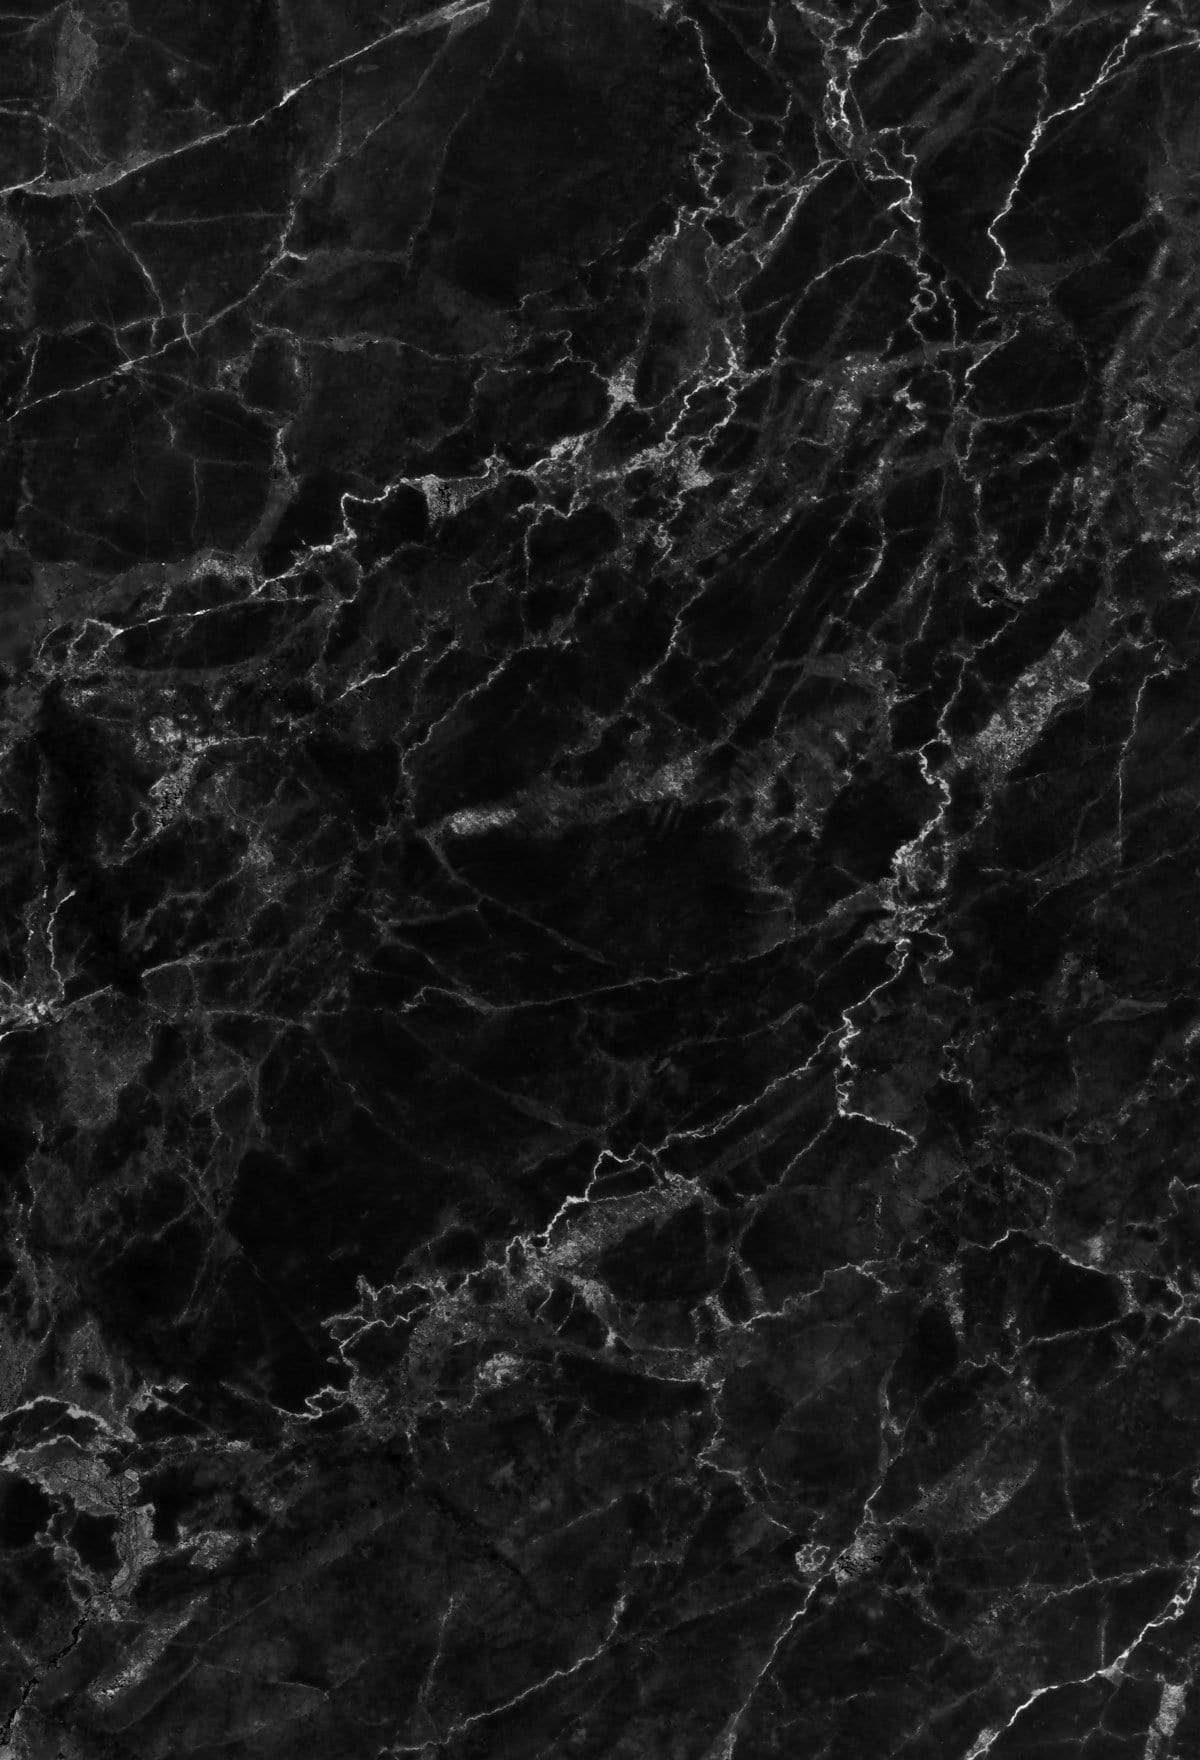
\includegraphics[width=\paperwidth,height=\paperheight]{marble.jpg}
		}%
}
\color{bronze}}
\newcommand{\clearbackground}{
	\backgroundsetup{
		scale=1,
		color=black,
		opacity=1,
		angle=0,
		contents={%
			\checkoddpage
			\ifoddpage
			\includegraphics[width=\paperwidth,height=\paperheight]{background_left.png}
			\else
			\includegraphics[width=\paperwidth,height=\paperheight]{background_right.png}		
			\fi
		}%
}
\color{black}}


\makeatletter
\def\ps@myPS{%
	\def\@oddfoot{\hspace*{24.5em}\thepage}
	\def\@evenfoot{\hspace*{28em}\thepage}%
	\def\@evenhead{\null\hfil\slshape\leftmark}%
	\def\@oddhead{{\slshape\rightmark}}}%
\makeatother
\pagestyle{myPS}

\title{Horus Heresy 2.0 Necrons}
\author{ingeanus}
\date{June 2024}

\begin{document}
	\renewcommand\thesection{}
	\renewcommand\thesubsection{}
	\renewcommand\thesubsubsection{}
	\contourlength{0.5pt} %how thick each copy is
	\contournumber{3}  %number of copies
	
	\maketitle
	
	\tableofcontents
	
	\newpage
	\section{The Necron Tombworlds}


\subsection{Building a Necron Army}

In games of the Horus Heresy: Age of Darkness, the models under a given player’s control are referred to as that player’s army. Each army is composed of a single Force Organisation chart (most commonly using the Crusade Force Organisation chart), which will include one or more Detachments. An army whose Primary Detachment is selected from any Army List is considered to have the Faction of that Primary Detachment (for example, an army whose Primary Detachment was selected from the Necrons List would be considered an Necron army). Units from various Sub-factions cannot be mixed in the same Detachment, unless a Special Rule or other ability permits this.

Other, non-Primary, Detachments in the same army may be selected from any other Army List - following any additional restrictions applied, such as the ones on the next page - but each Detachment may only include units from a single Army List, unless another Special Rule states otherwise.

When selecting a Primary Detachment, you must also choose a Sub-Faction for that detachment, in the form of a Necron Dynasty. Each Dynasty provides special bonuses and options for their units and determines the Alliance Levels between other Sub-Factions.

In addition, each Dynasty has a number of allied units that are usually attached to its Tomb Worlds, whether that be Triarch Praetorians watching over the slumbering necrons, a Destroyer Cult filling part of their ranks, or Flayed Ones lurking at the fringes. As such, a Primary Detachment is also allowed to incorporate a number of Allied Units without requiring an entire Allied Detachment be taken, so long as the number of points spent on Triarch, Destroyer, and Flayed models does not exceed 25\% of the army's total points.

\newpage
\begin{multicols}{2}
\subsection{Force Organisation Charts and Detachments}

The maximum and minimum number of units that may be included in a given army is defined by a Force Organisation chart, of which there is one basic chart available, the Crusade Force Organisation chart. 

Any Force Organisation chart is made up of one or more Detachments. A Force Organisation chart will always include one Primary Detachment, which must be selected, and may also include a number of optional Detachments which a player may choose to use or ignore. Each Detachment that a player chooses to use as part of their army must use a single Army List, which determines the Faction of that Detachment. Most optional Detachments are not required to be the same Faction as the Primary Detachment, but some Detachments may have special rules which require them to be of a certain Faction (and thus use a specific Army List). Detachments of different Factions in the same army will have additional special rules that determine how they interact (see \hyperref[allies]{the Allied Section}).

Each Detachment is composed of a number of boxes, each linked to one of the Battlefield Roles. Each of these boxes allows the player to make one selection from the section of their Army List that includes units of the same Battlefield Role. Dark boxes indicate Compulsory selections, which must be included as part of the Detachment, while the lighter boxes indicate optional choices, which are only included as part of the Detachment if the player in question chooses to do so.

Sometimes, a single choice in a Detachment may allow you to select more than one unit, or to vary the Battlefield Role of the unit selected. In all cases, such deviations from the normal procedure will be fully explained in the Force Organisation chart that the Detachment is part of.
 
Each unit selected to fill a box in any single Detachment must be chosen from the same Army List, and must be of the same Battlefield Role as that of the box. The unit profile in the Army List will dictate the number of points from the points limit that must be spent to add the unit to the player’s army. Players continue to spend points to fill boxes in Detachments within the chosen Force Organisation chart until either they run out of points, fill all boxes in all available Detachments or the player chooses to stop.

\subsection{Nodal Command Force}

The Tomb World's Nodal Command Force exemplifies the adaptable hierarchy of Necron military organization. Unlike traditional Terran militaries, there exists no static command structure within each Tomb World or sector. Instead, the organization adapts fluidly in response to each battle, campaign, or Harvest through the Nodal Command System. 

This system dynamically allocates hierarchy and command authority based on operational needs, ensuring both centralized control and decentralized tactical responsiveness, while threading many of the complex political natures of a Necron Tomb World at the same time.


\subsubsection{Nodal Command System}

The Nodal Command System assigns hierarchical values to nodes within the Necron force. These nodes, primarily Necron Lords, control various units and can shift their hierarchical roles as the situation demands. Hierarchical Command Levels within this system include Bronze, Silver, Gold, and Platinum nodes in extraordinary cases.

\fbox{\parbox{0.5\textwidth-4em}{When selecting the Nodal Command Force as your Primary Detachment, you must also determine the Command Level at which the Tomb World is operating at, with higher levels representing higher levels of escalation by the awakening Tomb World. This level determines what Force Organisation slots are available to you alongside what units are considered Compulsory. When selecting a higher level, you must take all of the Compulsory options for that level and all levels below it. For example, selecting a Decurion Formation has a Compulsory list of: 1 HQ (Silver), 1 HQ (Bronze), 2 Troops. Compulsory units for levels above yours are \textit{not} Compulsory, you may not include any Force Organization slots above your level at all — the Tomb World has not woken up to that degree.}}

\subsection{Command Levels and Battlefield Roles}

\subsubsection{Bronze-Level Command: Necron Line Formation}

Bronze-Level Command forms the primary response force against threats and curiosities identified by the Tomb World. These formations are usually summoned when a Primary Awakener Force encounters threats too potent or complex for them to handle, necessitating a more potent force. 

However, when such a response fails the Tomb World may seek to awaken a Silver-Level Command and subsume multiple Line Formations into a Decurion. When part of a Decurion Formation, each Line Formation is often referred to as a Cohort, with multiple Cohorts — traditionally two — forming a Legion.

The exact composition of a Line Formation varies by Tomb World and Dynasty, but a consistent feature is its overseeing Bronze-Level Necron Lord, possibly accompanied by their Lychguard retinue. General features include a number of Dynastic Warriors or Immortals that are supported by specialized units such as Cryptek Conclaves, Destroyer Cults, Flayed Ones, Canoptek constructs, and Triarch Praetorians.

\fbox{\parbox{0.5\textwidth-4em}{The Compulsory Headquarters unit for Necron Line Formations \textit{must} have the \quickref{Nodal Command} (Bronze) special rule.

\textbf{Primary Detachment: Necron Line Formation (Required)}
\begin{itemize}
	\item \textbf{Compulsory:} 1 HQ (Bronze),  1 Troop
	\item \textbf{Optional:} +2 Troops, +1 Elite, +2 Fast Attack, +1 Heavy Support, +4 Fortification
\end{itemize}}}

\subsubsection{Silver-Level Command: Necron Decurion Formation}

Silver-Level Commands are awakened by the Tomb World to address more strategically significant or politically worthy threats, creating what is termed a Decurion. This is a slow and dangerous process for any Tomb World during the 30th Millennium, and as such is never done lightly. 

Upon activation, a high-ranking or highly skilled Lord is traditionally anointed as Nemesor to lead the Decurion. This formation includes several Legions, each comprising multiple Line Formations with their own supporting elements and Bronze-Level Lords. The Decurion functions as a more traditional battlefield element, bringing specialized and advanced resources into play while coordinating multiple Line Formations for cohesive and effective responses to larger threats.

Should even this force prove insufficient, the Tomb World may escalate further by awakening a Gold-Level Command, subsuming multiple Decurions into a Tesserarion. In such cases, the title of Nemesor passes to the Overlord, with the Decurion acting as a medium force organization that coordinates individual Line Formations and relays data engrams to the Tesserarion’s leadership for efficient processing.

\fbox{\parbox{0.5\textwidth-4em}{The Compulsory Headquarters unit for Necron Decurion Formations \textit{must} have the \quickref{Nodal Command} (Silver) special rule.

\textbf{Extended Primary Detachment: Necron Decurion Formation (Optional)}
\begin{itemize}
	\item \textbf{Compulsory:} 1 HQ (Silver),  1 Troop
	\item \textbf{Optional:} +1 HQ, +2 Troops, +2 Elites, +1 Fast Attack, +1 Heavy Support
\end{itemize}}}

\subsubsection{Gold-Level Command: Necron Tesserarion Formation}

Gold-Level Command represents the highest echelon of the Necron battlefield hierarchy, led by the Tomb World's Gold-Level Overlord — or in extreme cases a Platinum-Level Phaeron. This command structure is activated only when events pose a significant threat to the Tomb World itself, as the risks associated with awakening so early from the Great Slumber to the Tomb World's Overlord and many of its extremely complex war machines are considerable.

Each Tesserarion encompasses several Decurions, each retaining their traditional elements. The number of Tesserarions can vary greatly depending on the campaign's scale, forming the might of the Tomb World’s military forces. While there is only one Overlord for each Tomb World, members of the Overlord's court may be given command of individual Gold-Level Command of Tesserarions, all under the Overlord's overarching command. If a Phaeron leads the campaign, each Tesserarion is often commanded by Overlords from his realms, although this is rare during the 30th Millennium, with a more likely situation leading the Phaeron to draw solely from the awakening Tomb World. Tesserarions deploy immensely powerful Necron war machines, including Monoliths, C’Tan shards, Seraptek Constructs, and more.

\fbox{\parbox{0.5\textwidth-4em}{The Compulsory Headquarters unit for Necron Tesserarion Formations \textit{must} have the \quickref{Nodal Command} (Gold) special rule.

\textbf{Extended Primary Detachment: Necron Tesserarion Formation (Optional)}
\begin{itemize}
	\item \textbf{Compulsory:} 1 HQ (Gold)
	\item \textbf{Optional:} +1 HQ, +1 Phaeron, +1 Troops, +1 Elite, +1 Fast Attack, +2 Heavy Supports
\end{itemize}}}

\end{multicols}
 
\newpage
{
\centering
\textbf{Nodal Command Force Detachment}

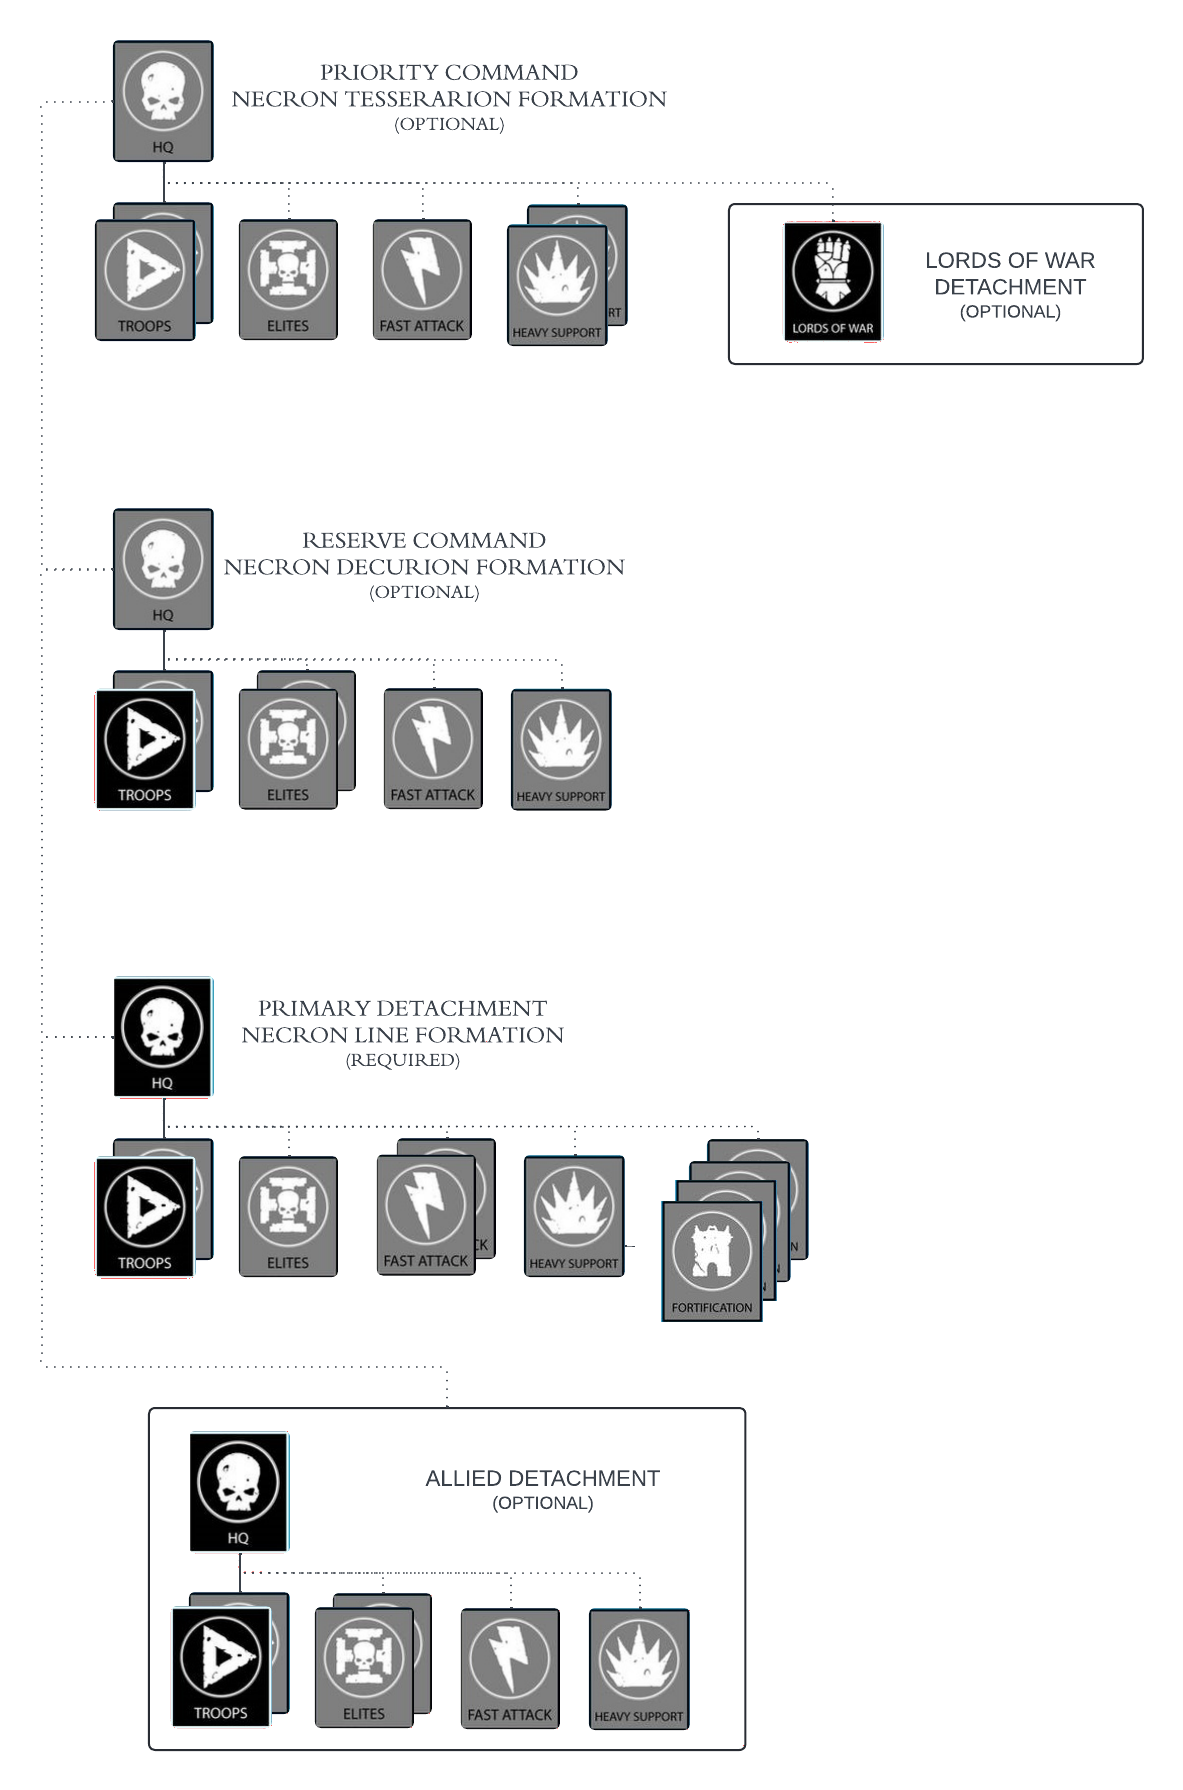
\includegraphics[width=470pt, height=700pt]{Org chart.png}

\begin{figure}
	\centering
	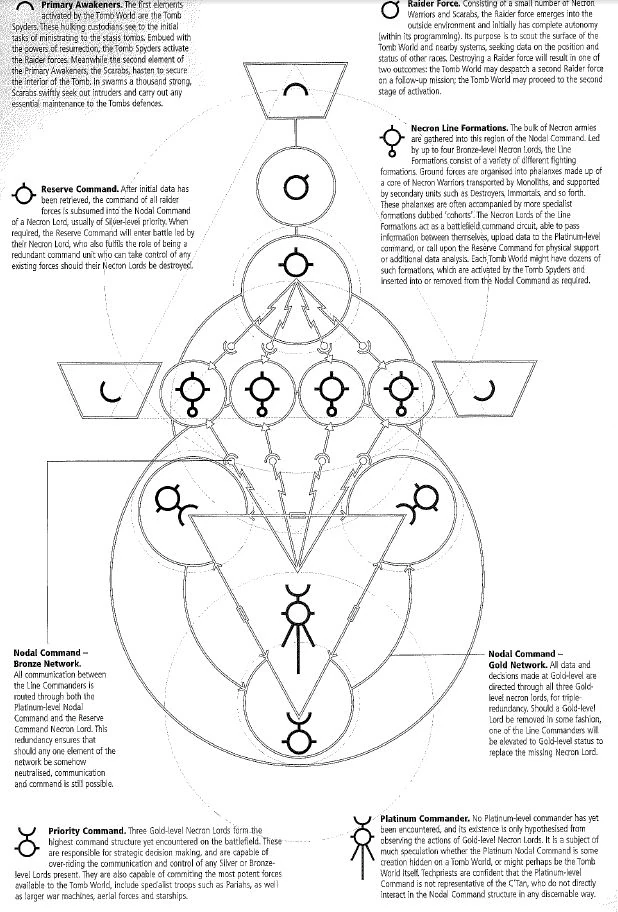
\includegraphics[width=515pt, height=750pt]{nodal.png}
\end{figure}
}

\newpage
\subsection{Warlords of the Necron Dynasties}

\subsubsection{Core Warlord Traits}
These Traits are available to any Character model selected as an army’s Warlord, regardless of Faction or Allegiance.

\begin{multicols}{2}

\textbf{Blood Handed}

\textit{Some warlords are only satisfied by the clash of blades and
the screams of the enemy as they fall before them. For such
warriors, strategy is but a means to an end, a tool by which
they can bring their forces into the brutal crucible of the melee
as soon as possible. There, in the heart of the battlefield, they
seek victory at any cost.}

\vspace*{1em}
Any combat with at least one friendly model within 12"
of this Warlord, or a combat which includes this Warlord,
gains a bonus of +1 to the number of Wounds caused for
the purposes of combat resolution. In addition, an army
whose Warlord has this Trait may make an additional
Reaction during their opponent’s Assault phase as long as
the Warlord has not been removed as a casualty.

\vspace*{1em}
\textbf{Stoic Defender}

\textit{This warlord is a rock, the hard place against which their foes
	are dashed and broken. When the enemy surges forth, they do
	not foolishly go to meet them, but dig in so that the foe may
	exhaust themselves against the defences prepared for them. In
	the end, victory comes to those willing to endure the fires of
	battle and emerge unscathed from its fury.}

\vspace*{1em}
Any friendly unit joined by a Warlord with this Trait
that makes a Shooting Attack will force the target unit to
make a Pinning test if it suffers any unsaved Wounds. In
addition, an army whose Warlord has this Trait may make
an additional Reaction during their opponent’s Shooting
phase as long as the Warlord has not been removed
as a casualty.

\vspace*{1em}
\textbf{Ever-vigilant}

\textit{Always ready to take advantage of the foe’s weakness, this
	warlord is a master of predicting and exploiting the flow of
	battle. Where the foe advances, this warlord falls back to
	better ground, where the foe retreats, this warlord advances,
	for victory is fickle and only falls into the grasp of those
	prepared for any eventuality.}

\vspace*{1em}
When this Warlord, and any unit it has joined, Runs
during the Movement phase, it adds the value of the
Warlord’s Initiative Characteristic, increased by 1, to
the distance moved, rather than the lowest Initiative
Characteristic in the unit. In addition, an army whose
Warlord has this Trait may make an additional Reaction
during their opponent’s Movement phase as long as the
Warlord has not been removed as a casualty.

\end{multicols}

\subsubsection{Necron Warlord Traits}
These Traits are available to any Character model selected as an army’s Warlord, regardless of Faction or Allegiance.

\begin{multicols}{2}
	
	Two or Three Necron Traits + 1 per Dynasty?
	
	\textbf{Sautekh: Hyperlogical Strategist}
	
	One of those ones that gives a reaction in each phase, versatile commander type
	
\end{multicols}

	
	\newpage
	\section[Necron Rules]{\superhuge{Necron Rules}}

\subsection[Special Rules]{\superlarge{Special Rules}}

\begin{multicols}{2}

\subsubsection{Annihilation Protocols} \label{Annihilation Protocols}

Only a single unit with Annihilation Protocol may be taken in armies using the Nodal Command Force Organisation Chart that contains any Fortifications.

\subsubsection{Awakening Protocols (Tier)} \label{Awakening Protocols}

This rule is accompanied by a tier of Bronze, Silver, Gold, and Platinum. Units with this rule can only be included in lists which contain an HQ model with the corresponding \quickref{Nodal Command} tier or higher. Some units have both of these special rules, in which case they cannot satisfy this rules requirements with their own \quickref{Nodal Command} special rule.

\subsubsection{Command Protocols} \label{Command Protocols}

At the start of the game, after both sides have deployed, each unit with this ability may select a Command Protocol that can be used during the game. Many options allow the player to roll a \textbf{Command Protocol check} for additional benefits. To do so, roll a Leadership Check, with success granting the listed effects. Failure causes the listed negative effect immediately.

\begin{tcolorbox}[breakable,enhanced,watermark graphics=white_marble.jpg,watermark opacity=1,watermark color=blue,watermark stretch=1,sharp corners]
\textbf{Protocol of Eternal Guardian}

This model may give up their Shooting Attacks this turn to use this power during the Movement Phase. Select a single friendly Necron unit within \quickref{Nodal Range} that has not moved yet and apply one of the following affects to the unit:

\begin{itemize}
	\itemsep 0pt
	\item The chosen unit improves its Cover Save by +1, or gains a 6+ Cover Save if it has none, but it may not Run this turn.
	\item The chosen unit can re-roll failed Cover Saves.
	\item When the chosen unit is targeted by a Shooting Attack, treat the distance between the attacking unit and the target as 3" longer than the actual distance for Shooting Attacks as long as it is in cover.
\end{itemize}

You may choose to make a Command Protocol check before using this power, if the check is successful two different options may be applied. If the Check is failed, the target unit suffers -1 to all Armour Saves until your next turn.
\end{tcolorbox}
	
\vfill\null
\columnbreak
\begin{tcolorbox}[breakable,enhanced,watermark graphics=white_marble.jpg,watermark opacity=1,watermark color=blue,watermark stretch=1,sharp corners]
\textbf{Protocol of Sudden Storm}

This model may give up their Shooting Attacks this turn to use this power during the Movement Phase. Select a single friendly Necron unit within \quickref{Nodal Range} that has not moved yet and apply one of the following affects to the unit:

\begin{itemize}
	\itemsep 0pt
	\item The chosen unit may immediately move a number of inches up to its unmodified Initiative Characteristic. If the chosen unit has mixed Initiative Characteristics, use the highest unmodified Characteristics.
	\item The chosen unit gains the Move Through Cover special rule and must re-roll failed Dangerous Terrain Tests until your next turn.
	\item The chosen unit's movement does not trigger enemy reactions until the end of your Movement Phase.
\end{itemize}

You may choose to make a Command Protocol check before using this power, if the check is successful two different options may be applied. If the Check is failed, the target unit may only move half their Movement (rounded down) this turn.
\end{tcolorbox}


\begin{tcolorbox}[breakable,enhanced,watermark graphics=white_marble.jpg,watermark opacity=1,watermark color=blue,watermark stretch=1,sharp corners]
\textbf{Protocol of Vengeful Stars}

This model may give up their Shooting Attacks this turn to use this power during the Shooting Phase. Select a single friendly Necron unit within \quickref{Nodal Range} that has not shot yet and apply one of the following affects to the unit:

\begin{itemize}
	\itemsep 0pt
	\item The chosen unit's Ranged Weapons gain the Ignores Cover rule until your next turn.
	\item The chosen unit's Ranged Weapons gain Breaching (6+) or increase the level of Breaching or Rending by 1 until your next turn.
	\item The chosen unit gains Relentless until your next turn.
\end{itemize}

You may choose to make a Command Protocol check before using this power, if the check is successful two different options may be applied. If the Check is failed, the target unit suffers -1 BS this turn.
\end{tcolorbox}

\vfill\null
\columnbreak
\begin{tcolorbox}[breakable,enhanced,watermark graphics=white_marble.jpg,watermark opacity=1,watermark color=blue,watermark stretch=1,sharp corners]
\textbf{Protocol of the Hungry Void}

This model may give up their Shooting Attacks this turn to use this power during the Shooting Phase. Select a single friendly Necron unit within \quickref{Nodal Range} apply one of the following affects to the unit:

\begin{itemize}
	\itemsep 0pt
	\item The chosen unit gains the Counter Charge (1) special rule until your next turn.
	\item The chosen unit's Melee Weapons gain Breaching (6+) or increase the level of Breaching or Rending by 1 until your next turn.
	\item The chosen unit gains the Furious Charge (1) special rule until your next turn.
\end{itemize}

You may choose to make a Command Protocol check before using this power, if the check is successful two different options may be applied. If the Check is failed, the target unit suffers -1 WS this turn.
\end{tcolorbox}

\begin{tcolorbox}[breakable,enhanced,watermark graphics=white_marble.jpg,watermark opacity=1,watermark color=blue,watermark stretch=1,sharp corners]
\textbf{Protocol of the Undying Legions}

This model may give up their Shooting Attacks this turn to use this power during the Shooting Phase. Select a single friendly Necron unit within \quickref{Nodal Range} and apply one of the following affects to the unit:

\begin{itemize}
	\itemsep 0pt
	\item The chosen unit gains a +1 bonus to \quickref{Reanimation Protocols} rolls until the next turn.
	\item The chosen unit's \quickref{Living Metal} ability has its It Will Not Die level increased by 2 levels (e.g. 5+ -> 3+) until  your next turn.
	\item The chosen unit ignores the first unsaved Wound it would take before your next turn.
\end{itemize}

You may choose to make a Command Protocol check before using this power, if the check is successful two different options may be applied. If the Check is failed, the target unit suffers -1 to \textit{Reanimation Protocol} rolls until next turn.
\end{tcolorbox}

\begin{tcolorbox}[breakable,enhanced,watermark graphics=white_marble.jpg,watermark opacity=1,watermark color=blue,watermark stretch=1,sharp corners]
\textbf{Protocol of the Conquering Tyrant}

This model may give up their Shooting Attacks this turn to use this power during the Movement Phase. Select a single friendly Necron unit within \quickref{Nodal Range} and apply one of the following affects to the unit:

\begin{itemize}
	\itemsep 0pt
	\item The chosen unit counts as being in \quickref{Nodal Range} of all units with the \quickref{Command Protocols} special ability until your next turn.
	\item The chosen unit gains the Hit \& Run ability until your next turn.
	\item The chosen unit gains a +2 bonus to Initiative Tests until your next turn.
\end{itemize}

You may choose to make a Command Protocol check before using this power, if the check is successful two different options may be applied. If the Check is failed, the target unit gains the Soulless Hordes (Bronze) trait this turn, if it did not already have it, and cannot ignore the Engrammatic Attack Patterns provision this turn.
\end{tcolorbox}

\subsubsection{Curse of Llandu'gor} \label{Curse of Llandu'gor}

A model with this special rule does not suffer the penalties for low Levels of Alliance (e.g. the Leadership penalty for \textit{By the Phaeron's}), although its allied units still do.

\subsubsection{Drawn to Blood} \label{Drawn to Blood}

A model with this special rule must start the game in Reserve or Infiltrate. Each time an enemy unit is completely destroyed the Necron player may move one unit with the Flayer Sub-type from Reserve into Ongoing Reserve, even if this means that a unit will appear turn One. Independent Characters may be attached to their units when entering.

\subsubsection{Nodal Command (Tier)} \label{Nodal Command}

This rule is accompanied by a tier of Bronze, Silver, Gold, and Platinum. Each tier provides a specified range known as Nodal Range, which many other abilities reference for their effects. Any unit within Nodal Range of this unit may use this model's Leadership in place of its own and units with the \quickref{Soulless Hordes} special rule may also ignore the Engrammatic Attack Patterns provision. The highest tier unit in your army \textit{must} be your Warlord.

\label{Nodal Range}
\begin{tabular}{|c|c|}
	\hline
	Tier & Nodal Range \\
	\hline
	Bronze & 6" \\
	Silver & 9" \\
	Gold & 12" \\
	Platinum & 12" \\
	\hline
\end{tabular}

\subsubsection{Mark of the Flayer} \label{Mark of the Flayer}

If this model or its attached unit destroys an enemy unit during the Assault Phase or fails a Morale check, immediately roll a D6 and apply the result as determined below: \\
\begin{tabular}{Z{11 pt} Z {0.42\textwidth}}
	D6 & Result \\
	1 & \textbf{Berserk:} The model is seized by murderous fury and unable to tell friend from foe. If part of an infantry unit, resolve D3 automatic hits on that unit using the model's weapons. If alone, the model suffers an immediate Wound, with no save allowed. \\
	2-5 & \textbf{In Control:} The model is able to control their madness by sheer force of will, giving no effect. \\
	6 & \textbf{Transfiguration:} The model is transfigured by madness, their auto-repair system distorting their form to express the malignance that consumes them. They gains the Fearless and Rage (1) trait until the end of combat. \\
\end{tabular}


\subsubsection{Entropic Strike (X)} \label{Entropic Strike}

When allocating wounds from a Wound Pool from a weapon with this special rule, lower the target model's Armour Save by 1 (e.g. 3+ -> 4+) permanently before making its save. Against Vehicles, an Armour Penetration roll equal to or greater than the listed value lowers the AV of all facings by 1 permanently before resolving the effects. Vehicles with lowered to an AV of 0 are destroyed and removed from the battlefield.

\subsubsection{Ethereal Interceptors} \label{Ethereal Interceptors}

This unit is may perform a separate Deep Strike Assault. Additionally, it may make use of the \quickref{Ethereal Interception} Advanced Reaction.

\subsubsection{Exile Ray (X)} \label{Exile Ray}

When firing a weapon with this special rule, a To Wound roll equal to or higher than the value listed wounds automatically, regardless of the target's Toughness, has the Instant Death special rule, and the victim must re-roll successful Invulnerable saves. Against Vehicles and Buildings, an Armour Penetration roll equal to or higher than the listed value inflicts a Penetrating Hit.

\subsubsection{Gauss (X)} \label{Gauss}

When firing a weapon with this special rule, a To Wound roll equal to or higher than the value listed wounds automatically, regardless of the target’s Toughness. Against vehicles and buildings, an Armour Penetration roll equal to or higher than the value listed inflicts a Glancing hit.

\subsubsection{Ground Lash} \label{Ground Lash}

When the weapon with this special rule is used to make a Shooting Attack, draw a line 1" inche wide from the model up to the listed range of the weapon — this is the projectile's path.

\begin{itemize}
	\item Each model (friend and enemy) caught in the path (except the firing model) suffers a hit. Models with the Flyer or Skimmer Sub-type are not affected.
	\item Units suffer a hit equal to the number of models caught under the line.
\end{itemize}

\subsubsection{Hyperspace Hunters} \label{Hyperspace Hunters}

A unit with this rule specializes in combat that makes use of movement through hyperspace pocket dimensions. In your Movement Phase, this unit may slip back into hyperspace instead of moving, as long as it did not arrive from Reserves this turn and is not locked in combat or Falling Back. If it does so, remove it from the board and place it into Ongoing Reserves. It can be assigned to a Deep Strike Assault as normal on your Next Player Turn. Models with this rule still make It Will Not Die rolls while placed back into reserves.

\subsubsection{Decurion/Tesserarion Nemesor} \label{Decurion Nemesor} \label{Tesserarion Nemesor}

The Decurion Nemesor / Tesserarion Nemesor special rule grants the following benefits:

\begin{itemize}
	\itemsep 0pt
	\item Rites of War: If a Detachment with the Necron Faction includes at least one model with the Decurion Nemesor special rule then that Detachment may select a single Rite of War. 
	\item Lord of the Legion: An army may only include a maximum of one model with this special rule per 1,000 points. This counts across all Detachments of an army.
	\item A model with this special rule may also include an Immortals, Pariah Lychguard, or Royal Lychguard unit as part of the same Force Organisation slot as the model with the Decurion Nemesor special rule, but must still meet the required \quickref{Awakening Protocols} tier.
\end{itemize}

If multiple units are eligible to take this ability, it can only be taken by those with the highest Nodal Command tier in the force that has not already taken this ability. 

\subsubsection{Path of Annihilation (X)} \label{Path of Annihilation}

When the weapon with this special rule is used to make a Shooting Attack, draw a line a number of inches wide equal to the Level in the brackets from the model up to the listed range of the weapon — this is the projectile's path.

\begin{itemize}
	\item For each model (friend and enemy) caught in the path (except the firing model), roll to hit as usual for a Shooting Attack, with each model suffering a hit if successful. Models with the Flyer Sub-type are not affected unless the controlling player decides to affect \textit{only} models with the Flyer Sub-type.
	\item If a Terrain piece, Building, or model with the Vehicle Unit Type or any model with 6 or more Wounds is successfully hit and does not suffer a Penetrating Hit or unsaved Wound the attack is blocked and its path will go no further than that model. The blocking model will however, suffer D3 additional hits.
	\item If a model with the Vehicle Unit Type and the Transport Sub-type suffers a Penetrating Hit from a weapon with this special rule, each unit Embarked on it suffers D6 hits from the weapon, in addition to any other effects. Any Wounds caused are allocated by the controller of the target unit.
	\item If a model with the Void Shields special rule is successfully hit by this attack and the Void Shield suffers a Penetrating Hit, immediately resolve another hit against the next Void Shield or the model itself if no Void Shields remain until an Armour Penetration roll is failed. If an Armour Penetration roll is failed against a Void shield the attack is blocked and its path will go no further than that model and it suffers no additional hits.
	\item Successful Invulnerable Saves and Feel No Pain Damage Mitigation rolls must be re-rolled. Successful Shrouded Damage Mitigation rolls are considered to have not hit the model.
\end{itemize}

\subsubsection{Necrodermis} \label{Necrodermis}

At the end of each of your turns, roll a number of D6 for each of your models equal to the amount of missing Wounds or Hull Points, but that has not been removed as a casualty or destroyed. On a roll equal to or greater than the number in brackets associated with the special rule, that model regains a Wound, or Hull Point, lost earlier in the game.

\subsubsection{Quake} \label{Quake}

All units hit by a weapon with the Quake type treat open ground as difficult terrain until the end of their controlling player's next turn.

\subsubsection{Reanimation Protocols} \label{Reanimation Protocols}

Whenever a friendly unit with Reanimation Protocols suffers unsaved wounds or resolves an effect causing wounds, and casualties have been removed, total the number of wounds that have been lost among models that were destroyed by this effect and put them into a \textbf{Reassembling Pool} and a second \textbf{Reassembling Pool} for wounds that have the Instant Death special rule.

For each wound in the \textbf{Reassembling Pool}, roll a D6, subtracting 1 for wounds in the Instant Death \textbf{Reassembling Pool}. This unit is \textbf{Reanimating} a wound for every 5+ roll. Each time such a unit \textbf{Reanimates} a wound, perform the following steps:

\begin{itemize}
	\itemsep 0pt
	\item If that unit is less than its Starting Strength, return one destroyed model to play in cohesion range with one wound remaining.
	\item Then, if that unit is at its Starting Strength and has models that are missing any wounds, select a model with the lowest remaining wounds; it regains one lost wound.
\end{itemize}

If this unit would be destroyed by the attack or effect, Reanimation Protocols still triggers; perform the process as normal, however after models have been returned from successful \textbf{Reanimation} rolls, if there are remaining wounds in the Wound Pool, continue allocating those to the newly \textbf{Reanimated} models until the Wound Pool for this attack is empty or all \textbf{Reanimation} rolls have been failed; these remaining wounds \textit{can} cause further Reanimation Protocols triggers if they destroy more models. Do note that effects that simply destroy the unit (e.g. Sweeping Advance) do not trigger Reanimation Protocols.

When assigning wounds to units that have multiple models missing any wounds, assign them to the models with the least amount of wounds. In case of ties, the attacking player decides which models to apply them to.

Certain effects can cause models to immediately begin \textbf{Reassembling} or \textbf{Reanimating}; \textbf{Reassembling} models create a \textbf{Reassembling Pool} equal to the lost wounds of those model and then roll for them as normal. \textbf{Reanimating} models immediately follow the steps for \textbf{reanimating} a number of times equal to the wounds of the destroyed model.

\subsubsection{Shroud of Despair} \label{Shroud of Despair}

Weapons with this special rule make To Wound rolls against the target's modified Leadership rather than Toughness. When attacking models with the Vehicle or Knight Unit-Type, add any Leadership penalties from special rules like Fear to the weapon's Strength. Successful Glancing Hits or Penetrating hits do not inflict lost Hull Points or roll on the Vehicle Damage Table, with a D6 being rolled instead: The model suffers the Crew Shaken effect on a result of 1-3 or the Crew Stunned effect on a 4-6.

\subsubsection{Soulless Hordes (X)} \label{Soulless Hordes}

Models with the Soulless Hordes special rule are subject to the Engrammatic Attack Patterns provision, which has effects dependent on the tier of the subtype:

\paragraph{Bronze}: During the controlling player's Shooting phase and Charge sub-phase, the a unit with the Soulless Hordes special rule must attempt a Shooting Attack if there is an enemy unit within range (they are not forced to charge), and must target the closest enemy unit possible that is within its line of sight and a valid target for a Shooting Attack or Charge. If two or more targets are equally close then the controlling player chooses which will be the target of a Shooting Attack or Charge. Similar to the Fearless rule, a unit with the Soulless Hordes special rule cannot choose to fail a Morale check due to the Our Weapons Are Useless special rule. In addition, a unit with the Soulless Hordes special rule may not make Reactions.

\paragraph{Silver}: During the controlling player's Shooting phase and Charge sub-phase, \textit{if} a unit with the Soulless Hordes special rule attempts a Shooting Attack and/or Charge they must target the closest enemy unit possible that is within its line of sight and a valid target for a Shooting Attack or Charge. If two or more targets are equally close then the controlling player chooses which will be the target of a Shooting Attack or Charge. Similar to the Fearless rule, a unit with the Soulless Hordes special rule cannot use any Reactions that grant a Cover Save, Armour Save or Invulnerable Save, and cannot choose to fail a Morale check due to the Our Weapons Are Useless special rule.

The \quickref{Nodal Command} trait is able to suppress this special rule's effects while in Nodal Range.

\subsubsection{Supersonic} \label{Supersonic}

A Flyer with this special rule may move up to triple its movement when Zooming.

\subsubsection{Teleportation Reserves} \label{Teleportation Reserves}

If a unit in your army has equipment that allows them to interact with Teleportation Reserves — such as the \quickref{Eternity Gate} — you may have any units from your army start out in Teleportation Reserves. Certain abilities and wargear allow you to bring units from Teleportation Reserves onto the Battlefield, move units into Teleportation Reserves, or otherwise interact with them and will be detailed in their respective sections. While in Teleportation Reserves a unit cannot use any Deep-Strike or other Reserve abilities and may only enter play through another unit or effect that would allow it.

In addition, while in Teleportation Reserves a unit is actively repaired by the Tomb World's vast resources and expertise: At the start of your Player Turn a unit in Teleportation Reserves reassembles a number of wounds equal to the amount of lost wounds from any models plus the amount of wounds among destroyed models in the unit.

\subsubsection{Tesla (X)} \label{Tesla}

When firing a weapon with this special rule, a To Hit roll equal to or higher than the value listed generates an additional 2 hits. These hits may be applie to the target unit, or to any unit within 2" of the target unit.

\subsubsection{Their Number is Legion} \label{Their Number is Legion}

When a model with this special rule rolls for \quickref{Reanimation Protocols}, re-roll unmodified results of 1. If a unit with this special rules has at least half of hits models within 6" of an Objective, they instead re-roll unmodified results of 1 or 2. Dynastic Warrior models increase this range by 1.

\subsubsection{Their Name is Death} \label{Their Name is Death}

If a model with this special rule has not moved or Run during the Movement phase of its controlling player’s turn then that model may re-roll failed To Wound rolls or unmodified Armour Penetration rolls of 1 or 2 with Gauss Weapons and failed To Hit rolls with Tesla Weapons.

\subsubsection{Tomb Guardians} \label{Tomb Guardians}

Only a single unit with the Tomb Guardians rule may be used in any army which is built using the Nodal Command Force Organisation Chart and does not contain any Fortifications, should the army contain Fortifications there is no limit.

\end{multicols}

\subsection[Unit Sub-types]{\superlarge{Unit Sub-types}}

\subsubsection{Living Metal} \label{Living Metal}

The following rules apply to all models with the Living Metal Unit Sub-type:

\begin{itemize}
	\item Models with the Living Metal Sub-type has the \quickref{Necrodermis} (5+).
	\item Successful Wounds inflicted by attacks with the Poisoned or Fleshbane special rules must be re-rolled against models with the Living Metal Sub-type.
	\item The Shock Pulse and Disruption special rules affect models with the Living Metal Sub-type.
	\item Models with the Living Metal Sub-type ignore Leadership penalties caused by the Anathema Sub-type.
	\item Models with the Living Metal Sub-type may not make Sweeping Advances, unless a rule specifies otherwise.
	\item Models with the Vehicle Unit-Type and the Living Metal Sub-type ignore the effects of Crew Shaken (but still lose a Hull Point).
	\item Models with Super-Heavy Vehicle Unit-Type and the Living metal Sub-type ignore the effects of any variant of the Lance and Armourbane special rules when resolving attacks made against it and reduce the results of all rolls on the Vehicle Damage Chart caused by weapon without the Destroyer type by 1.
\end{itemize} 

\subsubsection{Canoptek} \label{Canoptek}

Models with the Canoptek subtype gain the Fearless special rule. \\


\subsubsection{C'Tan} \label{C'Tan}

Models with the C'Tan Unit Sub-type gain the following effects:

\begin{itemize}
	\item Models with the C'Tan Unit Sub-type cannot be Pinned.
	\item Models with the C'Tan Unit Sub-type may fire Heavy and Ordnance weapons and counts as Stationary even if it moved in the preceding Movement phase, and may declare Charges as normal regardless of any Shooting Attacks made in the same turn.
	\item Models with the C'Tan Unit Sub-type are not affected by special rules that negatively modify their Characteristics (other than Wounds). Note that this does not affect modifiers to Strength and Toughness conferred by the Daemon Unit Type.
	\item Models with the C'Tan Unit Sub-type have the \quickref{Necrodermis} (4+) Special rule.
	\item Models with the C'Tan Unit Sub-type may only make Reactions triggered by models with the Armiger, Dreadnought, Primarch, Mechanised or Vehicle Unit Type, or	any model with a Wounds Characteristic of 8 or more and additionally do trigger reactions from models with the Gargantuan Unit Sub-type.
	\item Successful Wounds scored by attacks with the Poisoned (X) or Fleshbane special rules must be re-rolled against models with the C'Tan Unit Sub-type.
	\item Models with the C'Tan Sub-type ignore Leadership penalties caused by the Anathema Sub-type.
	\item A model with the C'Tan Unit Sub-type may attack with all weapons it has in each Shooting Attack it makes including as part of a Reaction.
	\item No model that does not have the C'Tan Unit Sub-type may join a unit that includes a model with the C'Tan Unit Sub-type, and no model with the C'Tan Unit Sub-type may join a unit that does not have the C'Tan Unit Sub-type.
	\item Models with the C'Tan Unit Sub-type have the Eternal Warrior, Fearless, and Night Vision Special Rules.
\end{itemize}

\subsubsection{Destroyer} \label{Destroyer}

The following rules apply to all models with the Destroyer Unit Sub-type:

\begin{itemize}
	\item All models gain the Preferred Enemy (Non-Necrons) special rule.
	\item All models with the Destroyer Sub-type ignore the Living Metal Sub-type's restriction on performing Sweeping Advances. 
\end{itemize}

\subsubsection{Flayer} \label{Flayer}

The following rules apply to all models with the Flayer Unit Sub-type:

\begin{itemize}
	\item All models gain the Hatred (Non-Necrons) special rule.
	\item All models gain the Fear (2) special rule.
	\item All models gain the Deep-Strike and Infiltrate special rule.
	\item All models with the Flayer Sub-type ignore the Living Metal Sub-type's restriction on performing Sweeping Advances.
\end{itemize}

\subsubsection{Floating} \label{Floating}

A unit that includes only models with the Floating Sub-type may ignore the effects of any and all terrain it passes over during movement, including passing over vertical terrain and Impassable Terrain without penalty or restriction. However, such units may not begin or end their movement in Impassable Terrain, and if beginning or ending their movement in Dangerous Terrain must take Dangerous Terrain tests as normal.

\subsubsection{Noble} \label{Noble}

A model with the Noble Sub-type gains the Independent Character special rule. \\

\subsubsection{Phaeron} \label{Phaeron}

The following rules apply to all models with the Phaeron Unit Sub-type:

\begin{itemize}
	\item All Phaerons have the following Special Rules: Eternal Warrior, Fearless, It Will Not Die (3+), Relentless
	\item Phaerons are not affected by special rules that negatively modify their Characteristics (other than Wounds) and, in addition, Phaerons always resolves Snap Shots at their normal BS.
	\item Any Hits inflicted by a Phaeron, as part of either Shooting Attacks or in close combat, are allocated by the Phaeron’s controlling player and not the controlling player of the target unit. These Hits should form a separate Wound Pool.
\end{itemize}

	
	\newpage
	\section{Necron Factions}

\subsection{Charnovokh}

\textbf{Advanced Reaction:}

\textbf{Dynasty Effect:}


\subsection{Maynarkh}

Flayed One Focus. All units can take Flensing Scarabs

\textbf{Advanced Reaction:}

\textbf{Dynasty Effect:}


\subsection{Mephrit}

Mephrit Dynasty Necron units gain the Necron Dynasty (Mephrit) special rule, which grants the Solar Fury advanced reaction and Stellar Destruction special rule, alongside providing access to certain pieces of wargear.

\textbf{Advanced Reaction (Solar Fury):} This Advanced Reaction may be made once per battle during the opposing player’s Shooting phase when any enemy unit declares a Shooting Attack targeting a friendly unit under the Reactive player’s control composed entirely of models with the Necron Dynasty (Mephrit) special rule. Once the Active player has resolved all To Hit and To Wound rolls, and Armour Saves are made, but before any Damage Mitigation rolls are made or casualties removed, the Reactive player may make a Shooting Attack, targeting the unit that triggered this Reaction, with all weapons increasing their AP by 1 but gaining the Gets Hot special rule. To Hit rolls for weapons that already possess the Gets Hot special rule trigger that special rule on a roll of 1 or 2 during this Shooting Attack, instead of only on a 1. A unit that makes a Solar Fury as part of a Solar Fury Reaction may not make any attacks indirectly (without line of sight) including weapons with the Barrage special rule or other weapon or special rule that otherwise ignore line of sight, and Vehicles may only fire Defensive weapons. Template weapons used as part of a Solar Fury Reaction use the Wall of Death rule instead of firing normally.

\textbf{Necron Dynasty (Mephrit) (Stellar Destructors):} When rolling for scatter for Blast weapons, instead of rolling 2D6 roll a D6.


\subsection{Mephrit-Ghiar}

Like Mephrit, but should be more.. guerilla?

\textbf{Advanced Reaction:}

\textbf{Dynasty Effect:}


\subsection{Nephrekh}

\textbf{Advanced Reaction:}

\textbf{Dynasty Effect:}


\subsection{Nihilakh}

\textbf{Advanced Reaction:}

\textbf{Dynasty Effect:}


\subsection{Novokh}

Novokh Dynasty Necron units gain the Necron Dynasty (Novokh) special rule, which grants the Blood Engrams advanced reaction and Awakened By Murder special rule, alongside providing access to certain pieces of wargear.

\textbf{Advanced Reaction (Blood Engrams):} This Advanced Reaction may be made once per battle in the opposing player’s turn, when any enemy unit with one or more models within 12" of a friendly unit made up entirely of models with the Legiones Astartes (Space Wolves) special rule is moved during the Movement phase. Once the enemy unit that triggered this Reaction has been moved, but before any other units are moved, a single friendly unit made up entirely of models with the Legiones Astartes (Space Wolves) special rule that can draw a line of sight to the enemy unit that moved may immediately move up to a number of inches equal to the highest Initiative Characteristic in the unit and then declare a Charge targeting the enemy unit that moved if it is within 12". A Charge declared as part of this Reaction is resolved immediately (the enemy unit may not declare any Reaction against this Charge), and if successful the combat will be fought as normal in the following Assault phase, with a Charging unit with the Legiones Astartes (Space Wolves) special rule gaining all the normal benefits of Charging.

\textbf{Necron Dynasty (Novokh) (Awakened By Murder):} In the Fight sub-phase, after casualties have been removed but before determining which side has won, if this unit has caused unsaved to the enemy unit it enters \textit{Engrammatic Blood Rage} until the end of the game. When in \textit{Engrammatic Blood Rage}, this unit gains the Fearless, Furious Charge(1), and Rage(1) special rules.

\subsection{Sautekhan}

Sautekhan Dynasty Necron units gain the Necron Dynasty (Sautekhan) special rule, which grants the TODO advanced reaction and Uncanny Artifice special rule, alongside providing access to certain pieces of wargear.

\textbf{Advanced Reaction:}

\textbf{Dynasty Effect (Uncanny Artifice):} Units with this special rule may give any of their weapons Master-Crafted for 10 pts/weapon. Additionally, units with this special rule gain the Stubborn special rule.


\subsection{Szarekhan}

Some can take Master-Crafted?

\textbf{Advanced Reaction:}

\textbf{Dynasty Effect:} Maybe Stubborn?


\subsection{Thokt}

\textbf{Advanced Reaction:}

\textbf{Dynasty Effect:} Rad effect?


\subsection{Triarch}

Triarch buffs? Command buffs?

\textbf{Advanced Reaction:}

\textbf{Dynasty Effect:}


\subsection{Destroyer Cult}

Madness effect? High loss effect?

\textbf{Advanced Reaction:}

\textbf{Dynasty Effect:}


\subsection{Flayed Ones}

Anti-infantry stuff?

\textbf{Advanced Reaction:}

\textbf{Dynasty Effect:}
	
	\newpage
	\usection{Wargear}

\usubsection{Melee Weapons} \label{Melee Weapons}

\usubsubsection{Hyperphase Sword} \label{Hyperphase Sword}
\noindent
\begin{tabular}{||m{110pt} m{30pt} m{31pt} m{55pt} m{12pt} m{12pt} m{210pt}||}
	\hline
	Name & & Range & Type & S & AP & Abilities \\
	\hline
	\quickref{Hyperphase Sword} &  & — & Melee & User & 3 & Rending (5+) \\
	\hline
\end{tabular}

\usubsubsection{Rod of Night} \label{Rod of Night}
\noindent
\begin{tabular}{||m{110pt} m{30pt} m{31pt} m{55pt} m{12pt} m{12pt} m{210pt}||}
	\hline
	Name & & Range & Type & S & AP & Abilities \\
	\hline
	\quickref{Rod of Night} (Melee) & & — & Melee & User & — & Energy Siphon, Haywire \\
	\quickref{Rod of Night} (Shooting) & & 24" & Assault 2 & 5 & — & Haywire, \quickref{Tesla} (6+) \\
	\hline
\end{tabular}
\label{Energy Siphon}
\textbf{Energy Siphon:} At the end of the Fight sub-phase, if the bearer successfully hit with one or more attacks using the Rod of Night, they may roll a D6. On a roll of 4+, they may do one of the following to a friendly model within 3":
\begin{itemize}
	\item Restore a lost Wound
	\item Restore a lost Hull Point
\end{itemize}
	

\usubsubsection{Staff of Light} \label{Staff of Light}
\noindent
\begin{tabular}{||m{110pt} m{30pt} m{31pt} m{55pt} m{12pt} m{12pt} m{210pt}||}
	\hline
	Name & & Range & Type & S & AP & Abilities \\
	\hline
	\quickref{Staff of Light} (Shooting) & & 18" & Assault 3 & 5 & 3 & — \\
	\quickref{Staff of Light} (Melee) & & — & Melee & User & 3 & Rending (6+) \\
	\hline
\end{tabular}

\usubsubsection{Voidblade} \label{Voidblade}
\noindent
\begin{tabular}{||m{110pt} m{30pt} m{31pt} m{55pt} m{12pt} m{12pt} m{210pt}||}
	\hline
	Name & & Range & Type & S & AP & Abilities \\
	\hline
	\quickref{Voidblade} &  & — & Melee & User & 4 & \quickref{Entropic Strike} (4+), Rending (6+) \\
	\hline
\end{tabular}

\usubsubsection{Voidscythe} \label{Voidscythe}
\noindent
\begin{tabular}{||m{110pt} m{30pt} m{31pt} m{55pt} m{12pt} m{12pt} m{210pt}||}
	\hline
	Name & & Range & Type & S & AP & Abilities \\
	\hline
	\quickref{Voidscythe} &  & — & Melee & x2 & 1 & \quickref{Entropic Strike} (2+), Brutal (2), Unwieldy, Two-Handed \\
	\hline
\end{tabular}

\usubsubsection{Warscythe}
\label{Warscythe}
\noindent
\begin{tabular}{||m{110pt} m{30pt} m{31pt} m{55pt} m{12pt} m{12pt} m{210pt}||}
	\hline
	Name & & Range & Type & S & AP & Abilities \\
	\hline
	\quickref{Warscythe} & x pts& — & Melee & +2 & 2 & Armourbane (Melee), Two-Handed \\
	\hline
\end{tabular}

\usubsubsection{Whip Coils}
\label{Whip Coils}
\noindent
\begin{tabular}{||m{110pt} m{30pt} m{31pt} m{55pt} m{12pt} m{12pt} m{210pt}||}
	\hline
	Name & & Range & Type & S & AP & Abilities \\
	\hline
	\quickref{Whip Coils} & & — & Melee & User & — & Reach (3) \\
	\hline
\end{tabular}



\usubsection{Ranged Weapons} \label{Ranged Weapons}

\usubsubsection{Gauntlet Weapons}

\label{Gauntlet of Fire} \label{Tachyon Arrow}
\noindent
\begin{tabular}{||m{110pt} m{30pt} m{31pt} m{55pt} m{12pt} m{12pt} m{210pt}||}
	\hline
	Name & & Range & Type & S & AP & Abilities \\
	\hline
	\quickref{Gauntlet of Fire} & x pts& Template & Assault 1 & 4 & 5 & — \\
	\quickref{Tachyon Arrow} & x pts& $\infty$ & Destroyer 1 & 10 & 1 & Brutal (2), One use \\
	\hline
\end{tabular}



\usubsubsection{Gauss Weapons}

\label{Gauss Blaster} \label{Gauss Flayer} \label{Gauss Reaper} \label{Relic Gauss Blaster}
\noindent
\begin{tabular}{||m{110pt} m{30pt} m{31pt} m{55pt} m{12pt} m{12pt} m{210pt}||}
	\hline
	Name & & Range & Type & S & AP & Abilities \\
	\hline
	\quickref{Gauss Flayer} & x pts& 24" & Rapid Fire 1 & 4 & 5 & \quickref{Gauss} (6+) \\
	\quickref{Gauss Reaper} & x pts& 12" & Assault 2 & 5 & 4 & \quickref{Gauss} (6+) \\
	\quickref{Gauss Blaster} & x pts& 24" & Rapid Fire 1 & 5 & 4 & \quickref{Gauss} (6+) \\
	\quickref{Relic Gauss Blaster} & & 30" & Rapid Fire 2 & 5 & 4 & \quickref{Gauss} (6+), Master-Crafted \\	
	\hline
\end{tabular}

\usubsubsection{Particle Weapons}

\label{Particle Caster} \label{Particle Beamer}
\noindent
\begin{tabular}{||m{110pt} m{30pt} m{31pt} m{55pt} m{12pt} m{12pt} m{210pt}||}
	\hline
	Name & & Range & Type & S & AP & Abilities \\
	\hline
	\quickref{Particle Caster} & & 12" & Pistol 1 & 6 & 5 & \\
	\quickref{Particle Beamer} & & 24" & Heavy 1 & 6 & 5 & Blast \\	
	\hline
\end{tabular}

\usubsubsection{Tesla Weapons}
\label{Tesla Carbine}
\noindent
\begin{tabular}{||m{110pt} m{30pt} m{31pt} m{55pt} m{12pt} m{12pt} m{210pt}||}
	\hline
	Name & & Range & Type & S & AP & Abilities \\
	\hline
	\quickref{Tesla Carbine} & & 24" & Assault 2 & 5 & — & \quickref{Tesla} (6+) \\	
	\hline
\end{tabular}


\usubsubsection{Transdimensional Weapons}
\label{Transdimensional Beamer}
\noindent
\begin{tabular}{||m{110pt} m{30pt} m{31pt} m{55pt} m{12pt} m{12pt} m{210pt}||}
	\hline
	Name & & Range & Type & S & AP & Abilities \\
	\hline
	\quickref{Transdimensional Beamer} & & 12" & Heavy 1 & 4 & 5 & \quickref{Exile Ray} (6+) \\	
	\hline
\end{tabular}


\usubsection{Technoarkana} \label{Technoarcana}

\paragraph*{Dispersion Shield} \label{Dispersion Shield}

Grants a 3+ Invulnerable Save, but the wielder never receives +1 Attack for fighting with two Melee weapons.

\paragraph*{Gloom Prism} \label{Gloom Prism}

This model gains the Anathema sub-type. Additionally, any psychic power targeting a unit within 3" of this model is nullified on a 4+. \\

\paragraph*{Mindshackle Scarabs} \label{Mindshackle Scarabs}

At the start of the Fight sub-phase, select a model in base contact with the bearer. The target must take a Leadership Check on 3D6. If the Check is failed, the victim strikes at his allies instead of attacking normally. During the Fight sub-phase, the target makes his attacks against his own unit (automatically hitting if they are the only model in the unit), resolved as normal with any abilities and penalties from his weapons (the controller of the Mindshackle Scarbs chooses which, if there is a choice). If the target is still alive, the victim returns to normal once all blows in that round of combat have been struck.

\paragraph*{Phylactery} \label{Phylactery}

Increase the models It Will Not Die level to 3+.

\paragraph*{Phase Shifter} \label{Phase Shifter}

Grants a 4+ Invulnerable Save.

\paragraph*{Shadow Ankh} \label{Shadow Ankh}

The bearer gains the Anathema sub-type.

\paragraph*{Resurrection Orb} \label{Resurrection Orb}

Once per battle, on your turn, the bearer can activate their Resurrection Orb. If it does, select one friendly unit with \quickref{Reanimation Protocols} within \quickref{Nodal Range}. The bearer of the Orb and the selected unit immediately \textcolor{violet}{\hyperref[Reanimation Protocols]{reassembles}} a number of wounds equal to the total number of missing wounds and number of wounds from all destroyed models.

\paragraph*{Semipternal Weave} \label{Sempiternal Weave}

Increase the model's save to 2+.

\paragraph*{Tesseract Labyrinth} \label{Tesseract Labyrinth}

One use only.

The bearer can use the Tesseract Labyrinth in lieu of making a Shooting or Close Combat attack this round. Choose a unit within 6". The unit must immediately roll a Wounds Check for each model based on their current remaining wounds or be trapped within the Labyrinth while the Necron Character remains alive.

This can also be used to carry a unit alongside the bearer. Select a unit to start the game inside the Tesseract Labyrinth. They can be disembarked as if they were in a Transport with no Special Abilities following the relevant rules. 

If paired with the \quickref{Mindshackle Scarabs} wargear, this can also be a unit chosen from an enemy faction. The unit is treated as a Distrusted Ally and still take up a relevent Force Org Slot. In narrative games, units that are captured at the end of the game can be included as well. Leave it your opponents as to whether it includes a Force Org Slot or points.

\paragraph*{Translocation Shroud} \label{Translocation Shroud}

The bearer's unit gains the Fleet (2) special rule. When moving, the bearer's unit can move over all other models and terrain as if they were open ground. However, they cannot end their move on top of other models and can only end their move on top of impassable terrain if it is possible to actually place the models on top of it.

\usubsection{Artefacts of the Aeons} \label{Artefacts of the Aeons}

TODO: This

	
	\newpage
	\section{Cryptek Conclaves}

When taking a Cryptek Conclave, a \textbf{Discipline} must be taken from the list below, which grants a number of options, abilities, and restrictions to the unit.

\subsection[Harbingers of Despair ]{Harbingers of Despair  \hrulefill X pts}

Psychomancers must take an \quickref{Abyssal Staff} when selecting the Harbingers of Despair as their Discipline.

\subsubsection{Abyssal Staff}
\label{Abyssal Staff}
\noindent
\begin{tabular}{||m{130pt} m{10pt} m{31pt} m{55pt} m{12pt} m{12pt} m{210pt}||}
	\hline
	Name & & Range & Type & S & AP & Abilities \\
	\hline
	\quickref{Abyssal Staff} (Shooting) & & Template & Assault 1 & 8 & 1 & Shroud of Despair \\
	\quickref{Abyssal Staff} (Melee) & & — & Melee & 8 & 1 & Shroud of Despair \\
	\hline
\end{tabular}

\textbf{Shroud of Despair:} To Wound rolls are made against the target's Leadership (modified by Fear) rather than Toughness. The attack has no effect against Vehicles.

\subsubsection[Atavindicator ]{Atavindicator  \hrulefill X pts}

The bearer can activate the Atavindicator at the end of their Movement: Target an enemy unit that does not have the Vehicle Unit Type within 18". The targeted unit must make a Leadership Check on 3D6. Failure causes each model in the unit to automatically hit itself with a S+1 AP — melee attack.

\subsubsection[Nightmare Shroud ]{Nightmare Shroud  \hrulefill X pts} 

The bearer gains the Fear (1) rule. Additionally, the Shroud may be used during the Shooting Phase instead of firing a weapon. Choose an enemy unit within 18" of the bearer. That unit must immediately take a Morale Check.

\subsubsection[Veil of Darkness ]{Veil of Darkness  \hrulefill X pts}

The bearer of the Veil of Darkness has the Deep Strike special rule. In addition, once per game, at the start of any friendly Movement phase, the bearer can use the Veil of Darkness to remove himself and his unit from the table, even if they are locked in combat. They then immediately arrive anywhere on the board using the rules for Deep Strike. The bearer also has the \quickref{Transpositional Defence} Advanced Reaction.



\subsection[Harbingers of Destruction ]{Harbingers of Destruction  \hrulefill X pts}

Plasmancers must take an \quickref{Eldritch Lance} when selecting the Harbingers of Destruction as their Discipline.

\subsubsection{Eldritch Lance}
\label{Eldritch Lance}
\noindent
\begin{tabular}{||m{130pt} m{10pt} m{31pt} m{55pt} m{12pt} m{12pt} m{210pt}||}
	\hline
	Name & & Range & Type & S & AP & Abilities \\
	\hline
	\quickref{Eldritch Lance} (Shooting) & & 36" & Assault 1 & 8 & 2 & Lance \\
	\quickref{Eldritch Lance} (Melee) & & — & Melee & User & 2 & Lance \\
	\hline
\end{tabular}

\subsubsection[Gaze of Flame ]{Gaze of Flame  \hrulefill X pts}

The bearer, and its unit, are treated as being armed with Defensive grenades.

\subsubsection[Plasmic Lance ]{Plasmic Lance  \hrulefill X pts}

Any Plasmancer may exchange their Eldritch Lance for a Plasmic Lance.
%TODO: Probably too weak

\label{Plasmic Lance}
\noindent
\begin{tabular}{||m{130pt} m{10pt} m{31pt} m{55pt} m{12pt} m{12pt} m{210pt}||}
	\hline
	Name & & Range & Type & S & AP & Abilities \\
	\hline
	\quickref{Plasmic Lance} (Shooting) & & 18" & Assault 3 & 7 & 3 & — \\
	\quickref{Plasmic Lance} (Melee) & & — & Melee & User & 3 & — \\
	\hline
\end{tabular}

\subsubsection[Solar Pulse ]{Solar Pulse  \hrulefill X pts}

Once per game, at the start of any turn, the bearer can use this special rule. When he does, the Night Fighting rules are not in effect for the remainder of the turn (if they were in effect). In addition, when this special rule is used, enemy units targeting the bearer or his unit can only fire Snap Shots until the start of the bearer’s next turn.

\subsubsection[Quantum Orb ]{Quantum Orb  \hrulefill X pts}

Once per battle, at the start of your turn, the bearer can activate this item. If it does, select one point on the battlefield anywhere within 24" of the bearer and place a marker at that point. At the start of your next turn, resolve a S8 AP 3 Large Blast hit directly on that location. %TODO: Reaction?


\subsection[Harbingers of Eternity ]{Harbingers of Eternity  \hrulefill X pts}

Chronomancers must take an \quickref{Aeonstave} when selecting the Harbingers of Eternity as their Discipline.

\subsubsection{Aeonstave}
\label{Aeonstave}
\noindent
\begin{tabular}{||m{130pt} m{10pt} m{31pt} m{55pt} m{12pt} m{12pt} m{210pt}||}
	\hline
	Name & & Range & Type & S & AP & Abilities \\
	\hline
	\quickref{Aeonstave} & & — & Melee & User & — & \quickref{Entropic Strike} (4+), Chronal Charge \\
	\hline
\end{tabular}
\textbf{Chronal Charge:} Models which suffer an unsaved Wound or loses a Hull Point from this weapon loses the Fleet special rule and has its Weapon Skill, Ballistic Skill, Initiative and Attack values reduced to 1 for the remainder of the game.

\subsubsection[Chronometron ]{Chronometron  \hrulefill X pts}

A model with a Chronometron can re-roll one of its D6 rolls each phase alongside granting a 6+ Invulnerable Save. If the bearer is in a unit, this ability can be used to instead re-roll one of the units D6 rolls each phase and provides the 6+ Invulnerable Save to the attached unit as well. In addition, the bearer may make use of the \quickref{Strategical Timeweaver} Advanced Reaction.

\subsubsection[Chronotendrils ]{Chronotendrils  \hrulefill X pts}

The bearer's movement speed increases to 9" and they gain the Hammer of Wrath (3) ability.

\subsubsection[Countertemporal Nanomines ]{Countertemporal Nanomines  \hrulefill X pts}

Charges made against the bearer or their attached unit are always considered Disordered Charges. In addition, when measuring range between the target unit and the charging unit, consider the range as 3" longer than the actual distance during the Charge Sub-Phase.

\subsubsection[Entropic Lance ]{Entropic Lance  \hrulefill X pts} \label{Entropic Lance}

Any Chronomancer may upgrade their Aeonstave to an Entropic Lance.

\noindent
\begin{tabular}{||m{130pt} m{10pt} m{31pt} m{55pt} m{12pt} m{12pt} m{210pt}||}
	\hline
	Name & & Range & Type & S & AP & Abilities \\
	\hline
	\quickref{Entropic Lance} (Shooting) & & Assault 1 & 18" & 7 & 3 & Brutal (2), \quickref{Entropic Strike} (2+) \\
	\quickref{Entropic Lance} (Melee) & & — & Melee & User & 3 & Brutal (2), \quickref{Entropic Strike} (2+) \\
	\hline
\end{tabular}

\subsubsection[Timesplinter Cloak ]{Timesplinter Cloak  \hrulefill X pts}

A model with a Timesplinter Cloak has a 3+ Invulnerable save.

\subsection[Harbingers of Storm ]{Harbingers of Storm  \hrulefill X pts}

Ethermancers must take an \quickref{Voltaic Staff} when selecting the Harbingers of Storm as their Discipline.

\subsubsection{Voltaic Staff}
\label{Voltaic Staff}
\noindent
\begin{tabular}{||m{130pt} m{10pt} m{31pt} m{55pt} m{12pt} m{12pt} m{210pt}||}
	\hline
	Name & & Range & Type & S & AP & Abilities \\
	\hline
	\quickref{Voltaic Staff} (Shooting) & & 12" & Assault 4 & 5 & — & Haywire \\
	\quickref{Voltaic Staff} (Melee) & & — & Melee & User & — & Haywire \\
	\hline
\end{tabular}

\subsubsection[Ether Crystal ]{Ether Crystal  \hrulefill X pts}

Any enemy unit arriving by Deep Strike within \quickref{Nodal Range} of the bearer suffers d6 S8 AP 5 hits. If they arrive within range of multiple Crystals, only increase the number of hits by 1 for each Crystal past the first.

\subsubsection[Living Lightning ]{Living Lightning  \hrulefill X pts}

At the beginning of the Assault Phase, each enemy unit within \quickref{Nodal Range} of the bearer suffers 1 S8 AP 5 hit. TODO: Reaction?

\subsubsection[Metalodermal Tesla Weave ]{Metalodermal Tesla Weave  \hrulefill X pts}

When an enemy unit successfully moves into assault with the Cryptek or his unit, the assaulting unit immediately suffers d6 S8 AP 5 hits.




\subsection[Harbingers of Technomancy ]{Harbingers of Technomancy  \hrulefill X pts}

Technomancers must take a \quickref{Staff of Light} when selecting the Harbingers of Technomancy as their Discipline. Additionally, they must purchase the \quickref{Rites of Reanimation} ability.

\subsubsection[Canoptek Cloak ]{Canoptek Cloak  \hrulefill X pts}

Increase the bearer's move to 12" and it gains the Fleet (1) rule alongside the Antigrav and Light sub-type.

\subsubsection[Canoptek Control Node ]{Canoptek Control Node  \hrulefill X pts}

Double your \quickref{Nodal Range} when determining whether a friendly Necron unit with the Canoptek Sub-Type is within it. TODO: Reaction to shoot back better?

\subsubsection[Fail-Safe Overcharger ]{Fail-Safe Overcharger  \hrulefill X pts}

At the start of the Movement Phase, this model may give up its Shooting attacks for this turn to use this power. If you do so, make a Leadership Check. Failure causes an immediate wound to the selected unit that only Invulnerability and Damage Mitigation rolls can prevent. Success allows you to select a single friendly Necron unit with the Canoptek Sub-Type with \quickref{Nodal Range} and apply one of the following effects to that unit.

\begin{itemize}
	\item The chosen unit gains +1 BS until the end of the next turn.
	\item The chosen unit gains +1 WS until the end of the next turn.
	\item The chosen unit gains +1 A until the end of the next turn.
	\item The chosen unit gains a 6+ Invulnerability Save until the end of the next turn.
	\item The chose unit gains +3 M until the end of the next turn.
\end{itemize}

You may attempt to apply multiple options at once to the same unit or to multiple units within \quickref{Nodal Range} by taking a cumulative -1 penalty to your Leadership Check for each option after the first. The same option may be taken multiple times. If applying options to multiple units, a failed check causes an immediate wound to each unit as described above.

\subsubsection[Phylacterine Hive ]{Phylacterine Hive  \hrulefill X pts}

Once per battle, when using your \quickref{Rites of Reanimation} ability, you may select a non-friendly unit with \quickref{Reanimation Protocols} (Such as Destroyer Cult or Flayer Virus units) to be affected.

\subsubsection{Rites of Reanimation} \label{Rites of Reanimation}

After this model has moved, select a friendly unit with \quickref{Reanimation Protocols} within \quickref{Nodal Range} on the bearer. That unit immediately \textcolor{violet}{\hyperref[Reanimation Protocols]{reassembles}} a number of wounds equal to the number of lost wounds plus the number of wounds from all destroyed models, but roll with a -1 modifier if the unit is not a Dynastic Warriors Phalanx.



\subsection[Harbingers of Transmogrification ]{Harbingers of Transmogrification  \hrulefill X pts}

Geomancers and Alchemists must take an \quickref{Tremorstave} when selecting the Harbingers of Transmogrification as their Discipline.

\subsubsection[Tremorstave]{Tremorstave \hrulefill X pts}
\label{Tremorstave}
\noindent
\begin{tabular}{||m{130pt} m{10pt} m{31pt} m{55pt} m{12pt} m{12pt} m{210pt}||}
	\hline
	Name & & Range & Type & S & AP & Abilities \\
	\hline
	\quickref{Tremorstave} (Shooting) & & 36" & Assault 1 & 4 & — & Blast, Pinning, Quake \\
	\quickref{Tremorstave} (Melee) & & — & Melee & User & — & Pinning \\
	\hline
\end{tabular}
\textbf{Quake:} After resolving all wounds, leave the Blast marker in place, or otherwise mark the area. This area now counts as Difficult Terrain until the start of the next turn of the player that made the attack.

\subsubsection[Harp of Dissonance ]{Harp of Dissonance  \hrulefill X pts}

\label{Harp of Dissonance}
\noindent
\begin{tabular}{||m{130pt} m{10pt} m{31pt} m{55pt} m{12pt} m{12pt} m{210pt}||}
	\hline
	Name & & Range & Type & S & AP & Abilities \\
	\hline
	\quickref{Harp of Dissonance} & & $\infty$ & Assault 1 & 6 & — & \quickref{Entropic Strike} (4+) \\
	\hline
\end{tabular}

\subsubsection[Cryptogeometric Adjuster ]{Cryptogeometric Adjuster  \hrulefill X pts}

At the start of your Shooting Phase, select an enemy unit within 18". Until the end of your next turn, whenever that unit measures distance for Shooting attacks or Charges, treat the distance between the attacking unit and the target as 6" longer than the actual distance for Shooting Attacks and 3" longer than the actual distance for Charges.


\subsubsection[Seismic Crucible]{Seismic Crucible \hrulefill X pts}

At the start of your Shooting Phase, select an enemy unit within 18". Until the start of your next turn, if that unit has the Vehicle Unit-Type it treats all terrain as Difficult terrain, otherwise it treats all terrain as Difficult and Dangerous terrain.


\section{Powers of the C'Tan} \label{Powers of the C'Tan}

\subsubsection{General Powers}

\subsubsection{Antimatter Meteor} \label{Antimatter Meteor}

\noindent
\begin{tabular}{||m{160pt} m{31pt} m{55pt} m{12pt} m{12pt} m{200pt}||}
	\hline
	Name & Range & Type & S & AP & Abilities \\
	\hline
	\quickref{Antimatter Meteor} (Shard) & 24" & Assault 1 & 8 & 3 & Large Blast \\
	\quickref{Antimatter Meteor} (Transcendent) & 48" & Assault 1 & 8 & 3 & Apocalyptic Blast \\
	\hline
\end{tabular}

\subsubsection{Cosmic Fire} \label{Cosmic Fire}

\noindent
\begin{tabular}{||m{160pt} m{31pt} m{55pt} m{12pt} m{12pt} m{200pt}||}
	\hline
	Name & Range & Type & S & AP & Abilities \\
	\hline
	\quickref{Cosmic Fire} (Shard) & Template & Assault 1 & 6 & 4 & Torrent (24") \\
	\quickref{Cosmic Fire} (Transcendent) & Template & Assault 2 & 6 & 4 & Torrent (36") \\
	\hline
\end{tabular}

\subsubsection{Entropic Touch} \label{Entropic Touch}

The C'Tan's weapons and powers gain the \quickref{Entropic Strike} trait at a level dependent on the C'Tan's level.

\textbf{Shard:} \quickref{Entropic Strike} (4+)

\textbf{Shard:} \quickref{Entropic Strike} (1+)

\subsubsection{Moulder of Worlds} \label{Moulder of Worlds}

\noindent
\begin{tabular}{||m{160pt} m{31pt} m{55pt} m{12pt} m{12pt} m{200pt}||}
	\hline
	Name & Range & Type & S & AP & Abilities \\
	\hline
	\quickref{Moulder of Worlds} (Shard) & 24" & Assault 3 & 4 & 5 & Massive Blast, Pinning, Shell Shock (1) \\
	\quickref{Moulder of Worlds} (Transcendent) & 48" & Assault 6 & 4 & 5 & Apocalyptic Blast, Pinning, Shell Shock (1) \\
	\hline
\end{tabular}

\subsubsection{Pyreshards} \label{Pyreshards}

\noindent
\begin{tabular}{||m{160pt} m{31pt} m{55pt} m{12pt} m{12pt} m{200pt}||}
	\hline
	Name & Range & Type & S & AP & Abilities \\
	\hline
	\quickref{Pyreshards} (Shard) & 18" & Assault 8 & 5 & — & Armourbane (Melta) \\
	\quickref{Pyreshards} (Transcendent) & 36" & Assault 16 & 5 & — & Armourbane (Melta) \\
	\hline
\end{tabular}

\subsubsection{Sentient Singularity} \label{Sentient Singularity}

All terrain within the listed range of the C'Tan is treated as Difficult and Dangerous Terrain for enemy units. Additionally, Deep Striking enemy units arriving within range are automatically considered Disordered.

\textbf{Shard:} 6"

\textbf{Transcendent:} 12"

\subsubsection{Seismic Assault} \label{Seismic Assault}

\noindent
\begin{tabular}{||m{160pt} m{31pt} m{55pt} m{12pt} m{12pt} m{200pt}||}
	\hline
	Name & Range & Type & S & AP & Abilities \\
	\hline
	\quickref{Seismic Assault} (Shard) & 24" & Assault 10 & 6 & 4 & Pinning \\
	\quickref{Seismic Assault} (Transcendent) & 48" & Assault 20 & 6 & 4 & Pinning \\
	\hline
\end{tabular}

\subsubsection{Sky of Falling Stars} \label{Sky of Falling Stars}

\noindent
\begin{tabular}{||m{160pt} m{31pt} m{55pt} m{12pt} m{12pt} m{200pt}||}
	\hline
	Name & Range & Type & S & AP & Abilities \\
	\hline
	\quickref{Sky of Falling Stars} (Shard) & 24" & Assault 3 & 7 & 4 & Barrage, Large Blast \\
	\quickref{Sky of Falling Stars} (Transcendent) & 48" & Assault 6 & 7 & 4 & Apocalyptic Barrage \\
	\hline
\end{tabular}

\subsubsection{Swarm of Spirit Dust} \label{Swarm of Spirit Dust}

The C'Tan gains Shrouded at a level dependent on its own level. Additionally, when targeted by a Shooting Attack, the range between an attacking unit and this model is considered to be a number of inches longer than actual, dependent on its level. In addition, when attacked by a weapon with the Barrage special rule a unit including one or more models with a distort field is always treated as though it was out of line of sight when scattering any attacks.

\textbf{Shard:} Shrouded (6+), +6"

\textbf{Shard:} Shrouded (5+), +9"

\subsubsection{Time's Arrow} \label{Time's Arrow}

\noindent
\begin{tabular}{||m{160pt} m{31pt} m{55pt} m{12pt} m{12pt} m{200pt}||}
	\hline
	Name & Range & Type & S & AP & Abilities \\
	\hline
	\quickref{Time's Arrow} (Shard) & 24" & Destroyer 1 & 10 & 1 & Precision Shot (6+) \\
	\quickref{Time's Arrow} (Transcendent) & 48" & Destroyer 2 & 10 & 1 & Precision Shot (5+) \\
	\hline
\end{tabular}

\subsubsection{Transdimensional Thunderbolt} \label{Transdimensional Thunderbolt}

\noindent
\begin{tabular}{||m{160pt} m{31pt} m{55pt} m{12pt} m{12pt} m{200pt}||}
	\hline
	Name & Range & Type & S & AP & Abilities \\
	\hline
	\quickref{Transdimensional Thunderbolt} (Shard) & 24" & Assault 1 & 9 & 1 & Tesla (6+) \\
	\quickref{Transdimensional Thunderbolt} (Transcendent) & 48" & Assault 2 & 9 & 1 & Tesla (5+) \\
	\hline
\end{tabular}

\subsubsection{Withering Worldscape} \label{Withering Worldscape}

Whilst the C'tan Shard is on the battlefield, all Difficult terrain is Dangerous for the enemy. If the terrain is already Dangerous, the Dangerous Terrain test is failed on a 1 or a 2.

\subsection{Specialist Powers}

\subsubsection{Gaze of Death} \label{Gaze of Death}

In its Shooting phase, in addition to using Powers of the C’tan, this model can target one non-vehicle enemy unit within 12" to which it has line of sight. The unit suffers a number of Wounds, dependent on the level of the C'Tan. Shard level causes wounds equal to 3D6 minus the target's Leadership while Transcendent causes 4D6. These are resolved at AP2 and with the Ignores Cover special rule. If at least one unsaved Wound is inflicted, the C’tan Shard of the Nightbringer immediately regains one Wound lost earlier in the battle.

\subsubsection{Lord of Fire (X)} \label{Lord of Fire}

All Flamer weapons (as well as Heat Rays, Burnas, Skorchas, Inferno Cannons and any other weapons which is described as using 'flame' or 'fire' as its effect or in its special rules) and weapons with the melta type fired within 12" of the C'tan Shard have a chance of exploding. Roll a D6 each time such a weapon is fired within range. On a roll equal or greater to this power's level, the weapon detonates. If carried by a non-vehicle model, the model is removed from play as a casualty with no saves. If mounted on a vehicle, it counts as Weapon Destroyed and causes the lose of a Hull Point. In either case, the shot(s) misfire and are lost.

\textbf{Shard:} Lord of Fire (6+)

\textbf{Transcendent:} Lord of Fire (5+)


\subsubsection{Gaze of the Abyss} \label{Gaze of the Abyss}

If this model would be targeted by a Shooting Attack or Charge, the attacking unit must immediately make a Morale Test. Additionally, the C'Tan has the Fear ability at a level dependent on its level.

\textbf{Shard:} Fear (2)

\textbf{Transcendent:} Fear (3)


\subsubsection{Grand Illusion} \label{Grand Illusion}

After all forces have been deployed and all Scout moves have been made, roll a dice dependent on the C'Tan's level, being a D3 for Shard and D6 for Transcendent. You can immediately redeploy this many units, subject to the normal deployment rules for the mission. This power can be used to move units into or out of, reserve.


\subsubsection{Voltaic Storm} \label{Voltaic Storm}

After this model has completed its movement, target an enemy Vehicle, Dreadnought, or Automata unit within 18" with this power. Roll a D6 to determine the effect, dependent on the C'Tan's level.

\begin{tabular}{|Z{15pt} Z{450pt}|}
	\hline
	D6 & Result \\
	\hline
	1 & No Effect \\
	2-3 & A Vehicle Unit Type that is part of the target unit suffers 1 Glancing Hit if Shard Level, or 2 if Transcendent level. Any other model suffers 1 or 2 Wounds respectively. Only Invulnerable Saves or Damage Mitigation rolls may be taken against these. \\
	4-5 &  A Vehicle Unit Type that is part of the target unit suffers 1 Penetrating Hit if Shard Level, or 2 if Transcendent level. Any other model suffers 1 or 2 Wounds respectively. Only Invulnerable Saves or Damage Mitigation rolls may be taken against these. Re-roll results of Crew Stunned and Explodes. \\
	6 &  A Vehicle Unit Type that is part of the target unit suffers 1 Penetrating Hi, or 2 if Transcendent level. Any other model suffers 1 or 2 Wounds respectively. Only Invulnerable Saves or Damage Mitigation rolls may be taken against these. \\
	\hline
\end{tabular}

\section{Reactions}

\subsection{Ethereal Interception} \label{Ethereal Interception}

If this unit is in Deep-Strike reserves, this reaction may be made after an enemy units arrives from Reserves and has finished all of their movement. The reacting unit immediately arrives from Reserves, following the rules for Deep Strike Assaults. Then, if it within Line of Sight of the triggering unit, it may make a Shooting attack against the triggering unit. This reaction may only be used once per turn for each unit with it. \\

\subsection{Strategical Timewaeaver} \label{Strategical Timeweaver}

When an opponent declares a Shooting Attack or Fights this unit or a unit it is attached to, this reaction may be declared. The triggering unit must re-roll all successful To Hit and To Wound rolls against the reacting unit until the end of the attack, keeping the second result. This re-roll occurs even if the triggering unit's rules (e.g. Shred, Hatred, etc.) have already re-rolled these dice. This reaction may only be used once per game, per unit.

\subsection{Transpositional Defence} \label{Transpositional Defence}

	
	\newpage
	\setbackground
	\section[Units]{\texorpdfstring{\centering\Huge Units}{Units}}
	\clearbackground
	\setbackground
{
	\centering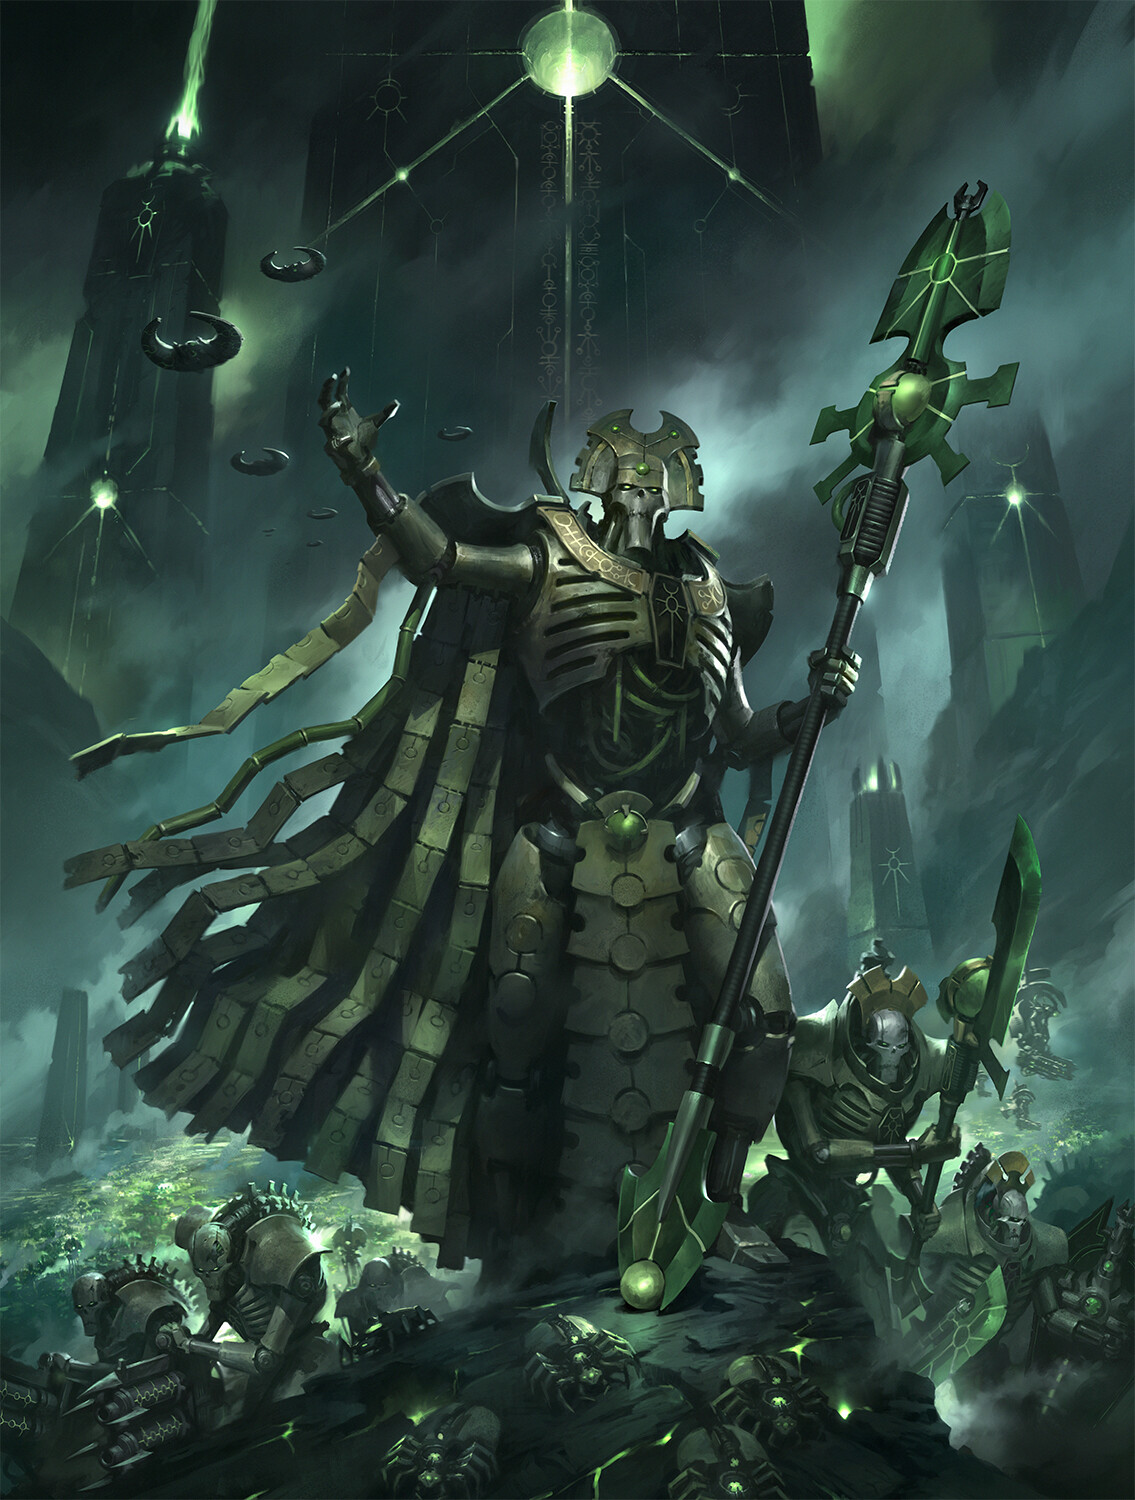
\includegraphics[height=530pt, width=400pt]{hq_art.jpg}
	\subsection{\texorpdfstring{\centering\Huge HQ}{HQ}}
	
	\centerline{\begin{minipage}{400pt}
			\centering
			'You stupid bastard, you got us box seats to a coup.’
			
			‘Well, the reviews were very good.'
			
			\vspace*{1em}
			\raggedleft Orikan the Diviner to Trazyn the Infinite
	\end{minipage}}
}

\newpage
\clearbackground
\subsubsection[Lord]{}

\fbox{\begin{imgminipage}{marble.jpg}[t]{0.2\textwidth}
		\color{white}
		\centering {\large HQ}
		
		\raggedright \small
		\color{black}
\end{imgminipage}}
\hspace{0.5em}
\begin{minipage}[t]{0.72\textwidth}
	{\large \textbf{Lord \dotfill 40 Points}}
	
	\begin{tabular}{m{165 pt} *{10}{c}}
		& M & WS & BS & S & T & W & I & A & Ld & Sv \\
		\hline
		Lord & 7 & 4 & 4 & 5 & 5 & 2 & 2 & 2 & 10 & 3+ \\
	\end{tabular}
	\small
	\begin{minipage}[t]{0.5\textwidth}
		\begin{flushleft}
		\vspace*{2em}
		\textbf{Unit Composition}
		\begin{itemize}
			\item 1 Lord
		\end{itemize}
		
		\textbf{Wargear}
		\begin{itemize}
			\item \quickref{Staff of Light}
		\end{itemize}
		\end{flushleft}
	\end{minipage}
	\begin{minipage}[t]{0.5\textwidth}
		\begin{flushleft}
		\vspace*{2em}
		\textbf{Unit Type}
		\begin{itemize}
			\item Infantry (Character, \quickref{Living Metal}, \quickref{Noble})
		\end{itemize}
		
		\textbf{Special Rules}
		\begin{itemize}
			\item \quickref{Command Protocols}
			\item \quickref{Nodal Command} (Bronze)
			\item \quickref{Reanimation Protocols}
			\item Relentless
		\end{itemize}
		\end{flushleft}
	\end{minipage}
	
	\vspace*{2em}
	\textbf{Weapons}
	
	\begin{tabular}{m{95 pt} *{4}{c} >{\raggedright\arraybackslash}p{130pt}}
		& Range & Type & S & AP & Abilities \\
		\hline
		\quickref{Staff of Light} & & &  &  &  \\
		— Shooting & 18" & Assault 3 & 5 & 3 & — \\
		— Melee & — & Melee & User & 3 & Rending (6+) \\
		\quickref{Hyperphase Sword} & — & Melee & User & 3 & Rending (5+) \\
		\quickref{Voidblade} & — & Melee & User & 4 & \quickref{Entropic Strike} (4+), Rending(6+) \\
		\quickref{Warscythe} & — & Melee & +2 & 2 & Armourbane (Melee), Two-Handed \\
		\quickref{Relic Gauss Blaster} & 30" & Rapid Fire 2 & 5 & 4 & \quickref{Gauss} (6+), Master-Crafted \\
	\end{tabular}
	
	\vspace*{2em}
	\textbf{Options}
	\begin{itemize}
		\item The Lord may exchange their \quickref{Staff of Light} for one of the following options:
		\begin{itemize}			
			\item \quickref{Hyperphase Sword} \dotfill -2 points
			\item \quickref{Voidblade} \dotfill +0 points
			\item \quickref{Warscythe} \dotfill +20 points
			\item \quickref{Warscythe} with in-built \quickref{Relic Gauss Blaster} \dotfill +30 points
		\end{itemize}
		\item The Lord may take any of the following options:
		\begin{itemize}
			\item \quickref{Gauntlet of Fire} \dotfill +10 points
			\item \quickref{Tachyon Arrow} \dotfill +150 points
			\item \quickref{Mindshackle Scarabs} \dotfill +20 points
			\item \quickref{Phase Shifter} \dotfill +25 points
			\item \quickref{Phylactery} \dotfill +10 points
			\item \quickref{Resurrection Orb} \dotfill +25 points
			\item \quickref{Translocation Shroud} \dotfill +10 points
		\end{itemize}
		\item The Lord may take equipment from the \quickref{Artefacts of the Aeons} list.
	\end{itemize}
\end{minipage}



\newpage
\subsubsection[Nemesor Lord]{}

\begin{minipage}[t]{0.72\textwidth}
	{\large \textbf{Nemesor Lord \dotfill 65 points}}
	
	\begin{tabular}{m{165 pt} *{10}{c}}
		& M & WS & BS & S & T & W & I & A & Ld & Sv \\
		\hline
		Nemesor Lord & 7 & 5 & 4 & 5 & 5 & 3 & 2 & 3 & 10 & 3+ \\
	\end{tabular}
	\small
	\begin{minipage}[t]{0.5\textwidth}
		\begin{flushleft}
		\vspace*{2em}
		\textbf{Unit Composition}
		\begin{itemize}
			\item 1 Nemesor Lord
		\end{itemize}
		
		\textbf{Wargear}
		\begin{itemize}
			\item \quickref{Staff of Light}
		\end{itemize}
		\end{flushleft}
	\end{minipage}
	\begin{minipage}[t]{0.5\textwidth}
		\begin{flushleft}
		\vspace*{2em}
		\textbf{Unit Type}
		\begin{itemize}
			\item Infantry (Character, \quickref{Living Metal}, \quickref{Noble})
		\end{itemize}
		
		\textbf{Special Rules}
		\begin{itemize}
			\item \quickref{Command Protocols}
			\item \quickref{Decurion Nemesor}
			\item \quickref{Nodal Command} (Silver)
			\item \quickref{Reanimation Protocols}
			\item Relentless
		\end{itemize}
		\end{flushleft}
	\end{minipage}
	
	\vspace*{2em}
	\textbf{Weapons}
	
	\begin{tabular}{m{95 pt} *{4}{c} >{\raggedright\arraybackslash}p{130pt}}
		& Range & Type & S & AP & Abilities \\
		\hline
		\quickref{Staff of Light} & & &  &  &  \\
		— Shooting & 18" & Assault 3 & 5 & 3 & — \\
		— Melee & — & Melee & User & 3 & Rending (6+) \\
		\quickref{Hyperphase Sword} & — & Melee & User & 3 & Rending (5+) \\
		\quickref{Voidblade} & — & Melee & User & 4 & \quickref{Entropic Strike} (4+), Rending(6+) \\
		\quickref{Warscythe} & — & Melee & +2 & 2 & Armourbane (Melee), Two-Handed \\
		\quickref{Relic Gauss Blaster} & 30" & Rapid Fire 2 & 5 & 4 & \quickref{Gauss} (6+), Master-Crafted \\
		\quickref{Rod of Night} & & &  &  &  \\
		— Shooting & 18" & Assault 2 & 5 & — & Haywire, \quickref{Tesla} (6+) \\
		— Melee & — & Melee & User & — & \quickref{Energy Siphon}, Haywire \\
	\end{tabular}
	
	\vspace*{2em}
	\textbf{Dedicated Transport}
	A Nemesor Lord may take a Catacomb Command Barge as a Dedicated Transport. As a Dedicated Transport this does not use up an additional Force Organisation slot, but its points cost must still be paid for as part of the army.
	
	\vspace*{2em}
	\textbf{Options}
	\begin{itemize}
		\item The Nemesor Lord may exchange their \quickref{Staff of Light} for one of the following options:
		\begin{itemize}			
			\item \quickref{Hyperphase Sword} \dotfill -2 points
			\item \quickref{Rod of Night} \dotfill +5 points
			\item \quickref{Voidblade} \dotfill +0 points
			\item \quickref{Warscythe} \dotfill +20 points
			\item \quickref{Warscythe} with in-built \quickref{Relic Gauss Blaster} \dotfill +30 points
		\end{itemize}
		\item A Nemesor Lord without a Two-Handed weapon may take the following:
		\begin{itemize}
			\item \quickref{Dispersion Shield} \dotfill +30 points
		\end{itemize}
		\item The Nemesor Lord may take any of the following options:
		\begin{itemize}
			\item \quickref{Gauntlet of Fire} \dotfill +10 points
			\item \quickref{Tachyon Arrow} \dotfill +150 points
			\item \quickref{Mindshackle Scarabs} \dotfill +20 points
			\item \quickref{Phase Shifter} \dotfill +25 points
			\item \quickref{Phylactery} \dotfill +10 points
			\item \quickref{Resurrection Orb} \dotfill +25 points
			\item \quickref{Sempiternal Weave} \dotfill +10 points
			\item \quickref{Tesseract Labyrinth} \dotfill +100 points
			\item \quickref{Translocation Shroud} \dotfill +10 points
		\end{itemize}
		\item The Nemesor Lord may take equipment from the \quickref{Artefacts of the Aeons} list.
	\end{itemize}
\end{minipage}
\hspace{0.5em}
\fbox{\begin{imgminipage}{marble.jpg}[t]{0.2\textwidth}
	\color{white}
	\centering {\large HQ}
	
	\raggedleft \small
	\color{black}
\end{imgminipage}}



\newpage
\subsubsection[Nemesor Overlord]{}

\fbox{\begin{imgminipage}{marble.jpg}[t]{0.2\textwidth}
		\color{white}
		\centering {\large HQ}
		
		\raggedright \small
		\color{black}
\end{imgminipage}}
\hspace{0.5em}
\begin{minipage}[t]{0.72\textwidth}
	{\large \textbf{Nemesor Overlord \dotfill 85 points}}
	
	\begin{tabular}{m{165 pt} *{10}{c}}
		& M & WS & BS & S & T & W & I & A & Ld & Sv \\
		\hline
		Nemesor Overlord & 7 & 5 & 5 & 5 & 5 & 4 & 2 & 3 & 10 & 3+ \\
	\end{tabular}
	\small
	\begin{minipage}[t]{0.5\textwidth}
		\begin{flushleft}
		\vspace*{2em}
		\textbf{Unit Composition}
		\begin{itemize}
			\item 1 Nemesor Overlord
		\end{itemize}
		
		\textbf{Wargear}
		\begin{itemize}
			\item \quickref{Staff of Light}
		\end{itemize}
		\end{flushleft}
	\end{minipage}
	\begin{minipage}[t]{0.5\textwidth}
		\begin{flushleft}
		\vspace*{2em}
		\textbf{Unit Type}
		\begin{itemize}
			\item Infantry (Character, \quickref{Living Metal}, \quickref{Noble})
		\end{itemize}
		
		\textbf{Special Rules}
		\begin{itemize}
			\item \quickref{Command Protocols}
			\item My Will Be Done
			\item \quickref{Nodal Command} (Gold)
			\item Overlord's Court
			\item \quickref{Reanimation Protocols}
			\item Relentless
			\item \quickref{Tesserarion Nemesor}
		\end{itemize}
		\end{flushleft}
	\end{minipage}
		
	\vspace*{2em}
	\textbf{Weapons}
	
	\begin{tabular}{m{95 pt} *{4}{c} >{\raggedright\arraybackslash}p{130pt}}
		& Range & Type & S & AP & Abilities \\
		\hline
		\quickref{Staff of Light} & & &  &  &  \\
		— Shooting & 18" & Assault 3 & 5 & 3 & — \\
		— Melee & — & Melee & User & 3 & Rending (6+) \\
		\quickref{Hyperphase Sword} & — & Melee & User & 3 & Rending (5+) \\
		\quickref{Voidblade} & — & Melee & User & 4 & \quickref{Entropic Strike} (4+), Rending(6+) \\
		\quickref{Voidscythe} & — & Melee & x2 & 1 & \quickref{Entropic Strike} (2+), Brutal (2), Unwieldy, Two-Handed \\
		\quickref{Warscythe} & — & Melee & +2 & 2 & Armourbane (Melee), Two-Handed \\
		\quickref{Relic Gauss Blaster} & 30" & Rapid Fire 2 & 5 & 4 & \quickref{Gauss} (6+), Master-Crafted \\
		\quickref{Rod of Night} & & &  &  &  \\
		— Shooting & 18" & Assault 2 & 5 & — & Haywire, \quickref{Tesla} (6+) \\
		— Melee & — & Melee & User & — & \quickref{Energy Siphon}, Haywire \\
	\end{tabular}
	
	\vspace*{2em}
	\textbf{Unit Rules}
	
	\textit{My Will Be Done:} A Nemesor Overlord automatically passes all Command Protocol checks.
	
	\textit{Overlord's Court:} When taking a Nemesor Overlord, you may also take one additional Lord or Nemesor Lord without using up an additional Force Organization Slot. 
	
	\vspace*{2em}
	\textbf{Dedicated Transport}
	A Nemesor Overlord may take a Catacomb Command Barge as a Dedicated Transport. As a Dedicated Transport this does not use up an additional Force Organisation slot, but its points cost must still be paid for as part of the army.
	
	\vspace*{2em}
	\textbf{Options}
	\begin{itemize}
		\item The Nemesor Overlord may exchange their \quickref{Staff of Light} for one of the following options:
		\begin{itemize}			
			\item \quickref{Hyperphase Sword} \dotfill -2 points
			\item \quickref{Rod of Night} \dotfill +5 points
			\item \quickref{Voidblade} \dotfill +0 points
			\item \quickref{Warscythe} \dotfill +20 points
			\item \quickref{Warscythe} with in-built \quickref{Relic Gauss Blaster} \dotfill +30 points
		\end{itemize}
		\item A Nemesor Overlord without a Two-Handed weapon may take the following:
		\begin{itemize}
			\item \quickref{Dispersion Shield} \dotfill +30 points
		\end{itemize}
		\item The Nemesor Overlord may take any of the following options:
		\begin{itemize}
			\item \quickref{Gauntlet of Fire} \dotfill +10 points
			\item \quickref{Tachyon Arrow} \dotfill +1+0 points
			\item \quickref{Mindshackle Scarabs} \dotfill +20 points
			\item \quickref{Phase Shifter} \dotfill +25 points
			\item \quickref{Phylactery} \dotfill +10 points
			\item \quickref{Resurrection Orb} \dotfill +25 points
			\item \quickref{Sempiternal Weave} \dotfill +10 points
			\item \quickref{Shadow Ankh} \dotfill +10 points
			\item \quickref{Tesseract Labyrinth} \dotfill +100 points
			\item \quickref{Translocation Shroud} \dotfill +10 points
		\end{itemize}
		\item The Nemesor Overlord may take equipment from the \quickref{Artefacts of the Aeons} list.
	\end{itemize}
\end{minipage}


\newpage
\subsubsection[Phaeron]{}

\begin{minipage}[t]{0.72\textwidth}
	{\large \textbf{Phaeron \dotfill X points}}
	
	\begin{tabular}{m{165 pt} *{10}{c}}
		& M & WS & BS & S & T & W & I & A & Ld & Sv \\
		\hline
		Phaeron & 7 & 6 & 6 & 5 & 5 & 4 & 2 & 4 & 10 & 3+ \\
	\end{tabular}
	\small
	\begin{minipage}[t]{0.5\textwidth}
		\begin{flushleft}
		\vspace*{2em}
		\textbf{Unit Composition}
		\begin{itemize}
			\item 1 Phaeron
		\end{itemize}
		
		\textbf{Wargear}
		\begin{itemize}
			\item \quickref{Staff of Light}
		\end{itemize}
		\end{flushleft}
	\end{minipage}
	\begin{minipage}[t]{0.5\textwidth}
		\begin{flushleft}
		\vspace*{2em}
		\textbf{Unit Type}
		\begin{itemize}
			\item Infantry (Character, \quickref{Living Metal}, \quickref{Noble}, \quickref{Phaeron}, Unique)
		\end{itemize}
		
		\textbf{Special Rules}
		\begin{itemize}
			\item \quickref{Command Protocols}
			\item My Will Be Done
			\item \quickref{Nodal Command} (Platinum)
			\item Phaeron's Court
			\item \quickref{Reanimation Protocols}
			\item \quickref{Tesserarion Nemesor}
		\end{itemize}
		\end{flushleft}
	\end{minipage}
	
	\vspace*{2em}
	\textbf{Weapons}
	
	\begin{tabular}{m{95 pt} *{4}{c} >{\raggedright\arraybackslash}p{130pt}}
		& Range & Type & S & AP & Abilities \\
		\hline
		\quickref{Staff of Light} & & &  &  &  \\
		— Shooting & 18" & Assault 3 & 5 & 3 & — \\
		— Melee & — & Melee & User & 3 & Rending (6+) \\
		\quickref{Hyperphase Sword} & — & Melee & User & 3 & Rending (5+) \\
		\quickref{Voidblade} & — & Melee & User & 4 & \quickref{Entropic Strike} (4+), Rending(6+) \\
		\quickref{Voidscythe} & — & Melee & x2 & 1 & \quickref{Entropic Strike} (2+), Brutal (2), Unwieldy, Two-Handed \\
		\quickref{Warscythe} & — & Melee & +2 & 2 & Armourbane (Melee), Two-Handed \\
		\quickref{Relic Gauss Blaster} & 30" & Rapid Fire 2 & 5 & 4 & \quickref{Gauss} (6+), Master-Crafted \\
		\quickref{Rod of Night} & & &  &  &  \\
		— Shooting & 18" & Assault 2 & 5 & — & Haywire, \quickref{Tesla} (6+) \\
		— Melee & — & Melee & User & — & \quickref{Energy Siphon}, Haywire \\
	\end{tabular}
	
	\vspace*{2em}
	\textbf{Unit Rules}
	
	\textit{My Will Be Done:} A Phaeron automatically passes all Command Protocol checks.
	
	\textit{Phaeron's Court:} When taking a Phaeron, you may also take up to 2 Nemesor Overlords without using up an additional Force Organization Slot. 
	
	\vspace*{2em}
	\textbf{Dedicated Transport}
	A Phaeron may take a Catacomb Command Barge as a Dedicated Transport. As a Dedicated Transport this does not use up an additional Force Organisation slot, but its points cost must still be paid for as part of the army.
	
	\vspace*{2em}
	\textbf{Options}
	\begin{itemize}
		\item The Phaeron may exchange their \quickref{Staff of Light} for one of the following options:
		\begin{itemize}			
			\item \quickref{Hyperphase Sword} \dotfill -2 points
			\item \quickref{Rod of Night} \dotfill +5 points
			\item \quickref{Voidblade} \dotfill +0 points
			\item \quickref{Warscythe} \dotfill +20 points
			\item \quickref{Warscythe} with in-built \quickref{Relic Gauss Blaster} \dotfill +30 points
		\end{itemize}
		\item A Phaeron without a Two-Handed weapon may take the following:
		\begin{itemize}
			\item \quickref{Dispersion Shield} \dotfill +30 points
		\end{itemize}
		\item The Phaeron may take any of the following options:
		\begin{itemize}
			\item \quickref{Gauntlet of Fire} \dotfill +10 points
			\item \quickref{Tachyon Arrow} \dotfill +190 points
			\item \quickref{Mindshackle Scarabs} \dotfill +20 points
			\item \quickref{Phase Shifter} \dotfill +25 points
			\item \quickref{Phylactery} \dotfill +10 points
			\item \quickref{Resurrection Orb} \dotfill +25 points
			\item \quickref{Sempiternal Weave} \dotfill +10 points
			\item \quickref{Shadow Ankh} \dotfill +10 points
			\item \quickref{Tesseract Labyrinth} \dotfill +100 points
			\item \quickref{Translocation Shroud} \dotfill +10 points
		\end{itemize}
		\item The Phaeron may take equipment from the \quickref{Artefacts of the Aeons} list.
	\end{itemize}
\end{minipage}
\hspace{0.5em}
\fbox{\begin{imgminipage}{marble.jpg}[t]{0.2\textwidth}
		\color{white}
		\centering {\large PHAERON}
		
		\raggedleft \small
		\color{black}
\end{imgminipage}}

\newpage
\subsubsection[Catacomb Command Barge]{}
\fbox{\begin{imgminipage}{marble.jpg}[t]{0.2\textwidth}
		\color{white}
		\centering {\large HQ}
		
		\raggedright \small
		\color{black}
\end{imgminipage}}
\hspace{0.5em}
\begin{minipage}[t]{0.72\textwidth}
	{\large \textbf{Catacomb Command Barge \dotfill X Points}}
	\begin{NiceTabular}{m{145 pt} *{2}{c} | *{3}{c} | c | c }
		& & & \cellgray{3}{Armour} & & & & \cellgray{1}{Transport} \\
		& M & BS & \cellgray{1}{Front} & \cellgray{1}{Side} & \cellgray{1}{Rear} & HP & \cellgray{1}{Capacity} \\
		\hline
		Catacomb Command Barge & 12 & 4 & \cellgray{1}{11} & \cellgray{1}{11} & \cellgray{1}{11} & 3 &\cellgray{1}{1} \\
	\end{NiceTabular}
	\small
	\begin{minipage}[t]{0.5\textwidth}
		\begin{flushleft}
		\vspace*{2em}
		\textbf{Unit Composition}
		\begin{itemize}
			\item 1 Catacomb Command Barge
		\end{itemize}
		
		\textbf{Wargear}
		\begin{itemize}
			\item Hull (Front) Mounted \quickref{Gauss Cannon}
			\item \quickref{Quantum Shielding}
		\end{itemize}
		\end{flushleft}
	\end{minipage}
	\begin{minipage}[t]{0.5\textwidth}
		\begin{flushleft}
		\vspace*{2em}
		\textbf{Unit Type}
		\begin{itemize}
			\item Vehicle (Chariot, \quickref{Living Metal}, Open-Topped, Skimmer, Transport)
		\end{itemize}
		
		\textbf{Special Rules}
		\begin{itemize}
			\item Command Wave
		\end{itemize}
		\end{flushleft}
	\end{minipage}
	
	\vspace*{2em}
	\textbf{Access Points}
	
	The Catacomb Command Barge has one Access Point on each side of the hull.
	
	\vspace*{2em}
	\textbf{Weapons}
	
	\begin{tabular}{m{95 pt} *{4}{c} >{\raggedright\arraybackslash}p{130pt}}
		& Range & Type & S & AP & Abilities \\
		\hline
		\quickref{Gauss Cannon} & 24" & Heavy 3 & 6 & 3 & \quickref{Gauss} (6+) \\
		\quickref{Tesla Cannon} & 30" & Heavy 3 & 6 & — & \quickref{Tesla} (6+) \\
	\end{tabular}
	
	\vspace*{2em}
	\textbf{Unit Rules}
	
	\textit{Command Wave}: All friendly units with the Necrons Faction within \quickref{Nodal Range} of a Catacomb Command Barge re-roll all failed Morale, Pinning and Fear tests.
	
	\vspace*{2em}
	\textbf{Options}
	\begin{itemize}
		\item The Catacomb Command Barge may exchange its \quickref{Gauss Cannon} for a:
		\begin{itemize}
			\item \quickref{Tesla Cannon} \dotfill +X points
		\end{itemize}
		\item A Catacomb Command Barge may take:
		\begin{itemize}
			\item \quickref{Quantum Shielding Matrix} \dotfill X points
		\end{itemize} 
	\end{itemize}
\end{minipage}


\newpage

\newpage
\subsubsection[Royal Warden]{}
\begin{minipage}[t]{0.72\textwidth}
	{\large \textbf{Royal Warden \dotfill X Points}}
	
	\begin{tabular}{m{165 pt} *{10}{c}}
		& M & WS & BS & S & T & W & I & A & Ld & Sv \\
		\hline
		Royal Warden & 7 & 4 & 4 & 5 & 5 & 2 & 2 & 2 & 10 & 3+ \\
	\end{tabular}
	\small
	\begin{minipage}[t]{0.5\textwidth}
		\begin{flushleft}
		\vspace*{2em}
		\textbf{Unit Composition}
		\begin{itemize}
			\item 1 Royal Warden
		\end{itemize}
		
		\textbf{Wargear}
		\begin{itemize}
			\item Close Combat Weapon
			\item \quickref{Relic Gauss Blaster}
		\end{itemize}
		\end{flushleft}
	\end{minipage}
	\begin{minipage}{0.5\textwidth}
		\vspace*{2em}
		\textbf{Unit Type}
		\begin{itemize}
			\item Infantry (Character, \quickref{Living Metal})
		\end{itemize}
		
		\textbf{Special Rules}
		\begin{itemize}
			\item \quickref{Awakening Protocols} (Silver)
			\item Independent Character
			\item \quickref{Reanimation Protocols}
			\item %TODO: Some buff for being a lieutenant
		\end{itemize}
	\end{minipage}
	
	\vspace*{2em}
	\textbf{Weapons}
	
	\begin{tabular}{m{95 pt} *{4}{c} >{\raggedright\arraybackslash}p{130pt}}
		& Range & Type & S & AP & Abilities \\
		\hline
		\quickref{Relic Gauss Blaster} & 30" & Rapid Fire 2 & 5 & 4 & \quickref{Gauss} (6+), Master-Crafted \\
	\end{tabular}
\end{minipage}
\hspace{0.5em}
\fbox{\begin{imgminipage}{marble.jpg}[t]{0.2\textwidth}
		\color{white}
		\centering {\large HQ}
		
		\raggedleft \small
		\color{black}
\end{imgminipage}}



\newpage
\subsubsection[Vargard]{}

\fbox{\begin{imgminipage}{marble.jpg}[t]{0.2\textwidth}
		\color{white}
		\centering {\large HQ}
		
		\raggedright \small
		\color{black}
\end{imgminipage}}
\hspace{0.5em}
\begin{minipage}[t]{0.72\textwidth}
	{\large \textbf{Vargard \dotfill X Points}}
	
	\begin{tabular}{m{165 pt} *{10}{c}}
		& M & WS & BS & S & T & W & I & A & Ld & Sv \\
		\hline
		Vargard & 7 & 5 & 4 & 5 & 5 & 2 & 2 & 3 & 10 & 3+ \\
	\end{tabular}
	\small
	\begin{minipage}[t]{0.5\textwidth}
		\begin{flushleft}
		\vspace*{2em}
		\textbf{Unit Composition}
		\begin{itemize}
			\item 1 Vargard
		\end{itemize}
		
		\textbf{Wargear}
		\begin{itemize}
			\item \quickref{Warscythe}
		\end{itemize}
		\end{flushleft}
	\end{minipage}
	\begin{minipage}[t]{0.5\textwidth}
		\begin{flushleft}
		\vspace*{2em}
		\textbf{Unit Type}
		\begin{itemize}
			\item Infantry (Character, \quickref{Living Metal})
		\end{itemize}
		
		\textbf{Special Rules}
		\begin{itemize}
			\item \quickref{Awakening Protocols} (Silver)
			\item Independent Character
			\item Lord's Retainer
			\item \quickref{Reanimation Protocols}
		\end{itemize}
		\end{flushleft}
	\end{minipage}
	
	\vspace*{2em}
	\textbf{Weapons}
	
	\begin{tabular}{m{95 pt} *{4}{c} >{\raggedright\arraybackslash}p{130pt}}
		& Range & Type & S & AP & Abilities \\
		\hline
		\quickref{Hyperphase Sword} & — & Melee & User & 3 & Rending (5+) \\
		\quickref{Warscythe} & — & Melee & +2 & 2 & Armourbane (Melee), Two-Handed \\
		\quickref{Relic Gauss Blaster} & 30" & Rapid Fire 2 & 5 & 4 & \quickref{Gauss} (6+), Master-Crafted \\	
	\end{tabular}

	\vspace*{2em}
	\textbf{Unit Rules}
	
	\textit{Lord's Retainer:} If a unit contains a Vargard as well as one or more models with the Noble Unit Sub-type, any Wounds which would be allocated to the Noble (even those caused by the Precision Strikes (X) or Sniper special rules) may instead	be allocated to a Vargard first.

	\vspace*{2em}
	\textbf{Options}
	\begin{itemize}
		\item The Vargard may exchange their \quickref{Warscythe} for one of the following options:
		\begin{itemize}			
			\item \quickref{Hyperphase Sword} and \quickref{Dispersion Shield} \dotfill 10 points
			\item \quickref{Relic Gauss Blaster} \dotfill -10 points
			\item \quickref{Warscythe} with in-built \quickref{Relic Gauss Blaster} \dotfill 10 points
		\end{itemize}
		\item The Vargard may take any of the following options:
		\begin{itemize}
			\item \quickref{Phase Shifter} \dotfill +25 points
			\item \quickref{Phylactery} \dotfill +10 points
			\item \quickref{Sempiternal Weave} \dotfill +10 points
		\end{itemize}
	\end{itemize}
\end{minipage}


\newpage
\subsubsection[Cryptek Conclave]{}

\begin{minipage}[t]{0.72\textwidth}
	{\large \textbf{Cryptek Conclave \dotfill X Points}}
	
	\begin{tabular}{m{165 pt} *{10}{c}}
		& M & WS & BS & S & T & W & I & A & Ld & Sv \\
		\hline
		Cryptek & 6 & 4 & 4 & 4 & 4 & 2 & 2 & 1 & 10 & 4+ \\
		Cryptek Lord & 6 & 4 & 4 & 5 & 5 & 2 & 2 & 1 & 10 & 3+ \\
	\end{tabular}
	\small
	\begin{minipage}[t]{0.5\textwidth}
		\begin{flushleft}
		\vspace*{2em}
		\textbf{Unit Composition}
		\begin{itemize}
			\item 1 Cryptek
		\end{itemize}
		
		\textbf{Wargear}
		\begin{itemize}
			\item Dependent on Conclave
		\end{itemize}
		\end{flushleft}
	\end{minipage}
	\begin{minipage}[t]{0.5\textwidth}
		\begin{flushleft}
		\vspace*{2em}
		\textbf{Unit Type}
		\begin{itemize}
			\item Infantry (Character, \quickref{Living Metal})
		\end{itemize}
		
		\textbf{Special Rules}
		\begin{itemize}
			\item Arkane Command
			\item \quickref{Awakening Protocols} (Bronze)
			\item Conclave Discipline
			\item Dynastic Advisors
			\item Independent Character
			\item \quickref{Reanimation Protocols}
		\end{itemize}
		\end{flushleft}
	\end{minipage}
	
	\vspace*{2em}	
	\textbf{Unit Rules}
	
	\textit{Arkane Command:} Cryptek models have the \quickref{Nodal Command} (Bronze) special rule, while Cryptek Lord models have the \quickref{Nodal Command} (Silver) special rule. This rule does not satisfy the pre-requisites for their own unit's \quickref{Awakening Protocols}.
	
	\textit{Conclave Discipline:} When taking a Cryptek Conclave, you must select a \quickref{Cryptek Conclave Discipline} for the unit. When selecting wargear from Disciplines, each piece of \textit{optional} wargear may only be taken once per unit. Models with differing Disciplines may never be part of the same unit. Before the battle, each model may be split off from his unit and be assigned to lead a different unit.
	
	\textit{Dynastic Advisors:} A Cryptek Conclave may be taken with a Lord, Nemesor Lord, Nemesor Overlord, or Phaeron unit as part of its Royal Court without using up an additional Force Organisation slot. If you do so, the number of models in this unit cannot exceed 1 for Lords, 2 for Nemesor Lords, 4 for Nemesor Overlords, and 5 for Phaerons.
	
	\vspace*{2em}
	\textbf{Options}
	\begin{itemize}
		\item The Cryptek Conclave may include:
		\begin{itemize}
			\item Up to an additional 4 Crypteks \dotfill X points each
		\end{itemize}
		\item Up to one Cryptek may be upgraded to a:
		\begin{itemize}
			\item Cryptek Lord \dotfill +X Points
		\end{itemize}
		\item A Cryptek or Cryptek Lord may take any of the following options:
		\begin{itemize}
			\item \quickref{Mindshackle Scarabs} \dotfill +20 points
			\item \quickref{Phase Shifter} \dotfill +25 points
			\item \quickref{Phylactery} \dotfill +10 points
		\end{itemize}
		\item A Cryptek Lord may take any of the following options:
		\begin{itemize}
			\item \quickref{Sempiternal Weave} \dotfill +10 points
			\item \quickref{Tesseract Labyrinth} \dotfill +100 points
			\item \quickref{Translocation Shroud} \dotfill +10 points
		\end{itemize}
	\end{itemize}
\end{minipage}
\hspace{0.5em}
\fbox{\begin{imgminipage}{marble.jpg}[t]{0.2\textwidth}
		\color{white}
		\centering {\large HQ}
		
		\raggedright \small
		\color{black}
\end{imgminipage}}


\newpage
\subsection{Dramatis Personae}

\subsubsection{Anrakyr the Traveller}

\newpage
\subsubsection{Trazyn the Infinite}

\newpage
\subsubsection{Orikan the Diviner}

\newpage
\subsubsection{Szarekh, the Silent King}
	
	\newpage
	\subsection{Troops}
\newpage
\subsubsection[Dynastic Warriors Phalanx]{}
\fbox{\begin{imgminipage}{marble.jpg}[t]{0.2\textwidth}
		\color{white}
		\centering {\large TROOPS}
				
		\raggedright \small
		The rank and file of the Necron
		armies are the Dynastic
		Warriors. Silent as the grave,
		Warriors move with slow, erratic,
		yet exacting movements. Despite
		this sluggishness, Warriors are
		capable of great accuracy at
		range and devastating blows up
		close. Like all Necrons, a
		Warrior's living metal
		necrodermis body is incredibly
		durable, capable of absorbing
		truly horrendous amounts of fire
		with hardly a scratch to show for
		it. When enough punishment is
		heaped on a Warrior to actually
		damage it, advanced self-repair
		protocols undo all but the most
		severe damage in moments.
		These seemingly indestructible
		machines carry Gauss Flayers
		which utilise theoretically
		impossible science to strip their
		target apart on a molecular level.
		These potent weapons can strip
		the adamantium from a battle
		tank's hull as surely as they strip
		the flesh from a man. Even
		Power Armour and the enhanced
		constitution of an Astartes
		provide limited defence.
		While the Necron nobility
		retained their personalities and
		intellects intact, their Warriors
		did not come through bio-
		transference so fortunate.
		Warriors possess but a dim
		spark of life, relying in battle on
		orders given through the Nodal
		Command network and
		programmed attack patterns
		rather than any self-direction or
		intellect.
		\color{black}
\end{imgminipage}}
\hspace{0.5em}
\begin{minipage}[t]{0.72\textwidth}
	{\large \textbf{Dynastic Warrior Phalanx \dotfill X Points}}
	
	\begin{tabular}{m{165 pt} *{10}{c}}
		 & M & WS & BS & S & T & W & I & A & Ld & Sv \\
		 \hline
		Dynastic Warrior & 5 & 4 & 4 & 4 & 4 & 1 & 2 & 1 & 10 & 4+ \\
	\end{tabular}
	\small
	\begin{minipage}[t]{0.5\textwidth}
		\begin{flushleft}
		\vspace*{2em}
		\textbf{Unit Composition}
		\begin{itemize}
			\item 10 Dynastic Warriors
		\end{itemize}
	
		\textbf{Wargear}
		\begin{itemize}
			\item Close Combat Weapon
			\item \quickref{Gauss Flayer}
		\end{itemize}
		\end{flushleft}
	\end{minipage}
	\begin{minipage}[t]{0.5\textwidth}
		\begin{flushleft}
		\vspace*{2em}
		\textbf{Unit Type}
		\begin{itemize}
			\item Infantry (Line, \quickref{Living Metal})
		\end{itemize}
		
		\textbf{Special Rules}
		\begin{itemize}
			\item \quickref{Reanimation Protocols}
			\item \quickref{Soulless Hordes} (Bronze)
			\item Their Number is Legion
		\end{itemize}
		\end{flushleft}
	\end{minipage}

	\vspace*{2em}
	\textbf{Weapons}
	
	\begin{tabular}{m{95 pt} *{4}{c} >{\raggedright\arraybackslash}p{130pt}}
		& Range & Type & S & AP & Abilities \\
		\hline
		\quickref{Gauss Flayer} & 24" & Rapid Fire & 4 & 5 & \quickref{Gauss} (6+)  \\
		\quickref{Gauss Reaper} & 12" & Assault 2 & 5 & 4 & \quickref{Gauss} (6+)  \\
	\end{tabular}

	\vspace*{2em}
	\textbf{Unit Rules}
	
	\textit{Their Number is Legion}: When rolling for \quickref{Reanimation Protocols}, unmodified rolls of 1 may be re-rolled.


	\vspace*{2em}
	\textbf{Dedicated Transport}
	A Dynastic Warrior Phalanx may take a Night Scythe as a Dedicated Transport if it numbers no more than 15 models, or a Ghost Ark as a Dedicated Transport if it numbers no more than 10 models. As a Dedicated Transport this does not use up an additional Force Organisation slot, but its points cost must still be paid for as part of the army.

	\vspace*{2em}
	\textbf{Options}
	\begin{itemize}
		\item The Dynastic Warrior Phalanx may include:
		\begin{itemize}
			\item Up to an additional 10 Dynastic Warriors \dotfill X points each
		\end{itemize}
		\item The entire unit may exchange their \quickref{Gauss Flayer} for a:
		\begin{itemize}
			\item \quickref{Gauss Reaper} \dotfill 0 points each
		\end{itemize}
	\end{itemize}
\end{minipage}


\newpage
\subsubsection[Immortals Phalanx]{}
\begin{minipage}[t]{0.72\textwidth}
	{\large \textbf{Immortal Phalanx \dotfill X Points}}
	
	\begin{tabular}{m{165 pt} *{10}{c}}
		& M & WS & BS & S & T & W & I & A & Ld & Sv \\
		\hline
		Immortals & 6 & 4 & 4 & 4 & 5 & 1 & 2 & 1 & 10 & 3+ \\
	\end{tabular}
	\small
	\begin{minipage}[t]{0.5\textwidth}
		\begin{flushleft}
		\vspace*{2em}
		\textbf{Unit Composition}
		\begin{itemize}
			\item 5 Immortals
		\end{itemize}
		
		\textbf{Wargear}
		\begin{itemize}
			\item Close Combat Weapon
			\item \quickref{Gauss Blaster}
		\end{itemize}
		\end{flushleft}
	\end{minipage}
	\begin{minipage}[t]{0.5\textwidth}
		\begin{flushleft}
		\vspace*{2em}
		\textbf{Unit Type}
		\begin{itemize}
			\item Infantry (Line, \quickref{Living Metal})
		\end{itemize}
		
		\textbf{Special Rules}
		\begin{itemize}
			\item \quickref{Awakening Protocols} (Bronze)
			\item \quickref{Reanimation Protocols}
			\item \quickref{Soulless Hordes} (Silver)
		\end{itemize}
		\end{flushleft}
	\end{minipage}
		
	\vspace*{2em}
	\textbf{Weapons}
	
	\begin{tabular}{m{95 pt} *{4}{c} >{\raggedright\arraybackslash}p{130pt}}
		& Range & Type & S & AP & Abilities \\
		\hline
		\quickref{Gauss Blaster} & 24" & Rapid Fire & 5 & 4 & \quickref{Gauss} (6+)  \\
		\quickref{Tesla Carbine} & 24" & Assault 2 & 5 & — & \quickref{Tesla} (6+)  \\
	\end{tabular}
	
	\vspace*{2em}
	\textbf{Dedicated Transport}
	An Immortal Phalanx may take a Night Scythe as a Dedicated Transport. As a Dedicated Transport this does not use up an additional Force Organisation slot, but its points cost must still be paid for as part of the army.
	
	\vspace*{2em}
	\textbf{Options}
	\begin{itemize}
		\item The Immortal Phalanx may include:
		\begin{itemize}
			\item Up to an additional 5 Immortals \dotfill X points each
		\end{itemize}
		\item The entire unit may exchange their \quickref{Gauss Blaster} for a:
		\begin{itemize}
			\item \quickref{Tesla Carbine} \dotfill 0 points each
		\end{itemize}
	\end{itemize}
\end{minipage}
\hspace{0.5em}
\fbox{\begin{imgminipage}{marble.jpg}[t]{0.2\textwidth}
		\color{white}
		\centering {\large TROOPS}
		
		\raggedleft \small
		As the shock troops of a Tomb
		World's armies, Immortals have
		a far wider range and depth of
		reaction than Warriors, for they
		have retained much of their
		tactical and strategic experience
		from eons ago. Indeed, in many
		ways, the biotransference to
		machine bodies and minds only
		sharpened the Immortals' ability
		to prosecute war in an efficient
		fashion. This is not to say that
		Immortals do not have
		shortcomings. Like all Dynastic
		Legions, they are still inescapably
		tied to the Nodal Command
		matrix and are reliant upon it for
		more advanced order.
		In life, Immortals were the
		professional soldiery of the
		Necrontyr empire. In death, they
		surpass the Warriors in nearly
		every way. Possessed of even
		more resilient frames, Necron
		Immortals prove almost
		impervious to small arms. Their
		training and experience in combat
		survived the process of bio-
		transference undiminished, and
		Immortals seem to have retained
		a brighter spark of intellect than
		their less favoured brethren,
		although only in regard to the
		practice of war. Outside of
		combat, Immortals display about
		as much personality as a
		monotask Servitor. Immortals
		are typically armed with Gauss
		Blasters, weapons even deadlier
		than the Gauss Flayers used by
		Warriors.
		\color{black}
\end{imgminipage}}
	
	\newpage
	\subsection{Elites}

\newpage
\subsubsection[Pariah Lychguard Phalanx]{}
\fbox{\begin{imgminipage}{marble.jpg}[t]{0.2\textwidth}
		\color{white}
		\centering {\large ELITES}
		
		\raggedright \small
		\color{black}
\end{imgminipage}}
\hspace{0.5em}
\begin{minipage}[t]{0.72\textwidth}
	{\large \textbf{Pariah Lychguard Phalanx \dotfill X Points}}
	
	\begin{tabular}{m{165 pt} *{10}{c}}
		& M & WS & BS & S & T & W & I & A & Ld & Sv \\
		\hline
		Pariah Lychguard & 7 & 4 & 4 & 5 & 5 & 1 & 2 & 1 & 10 & 3+ \\
	\end{tabular}
	\small
	\begin{minipage}[t]{0.5\textwidth}
		\begin{flushleft}
		\vspace*{2em}
		\textbf{Unit Composition}
		\begin{itemize}
			\item 5 Pariah Lychguard
		\end{itemize}
		
		\textbf{Wargear}
		\begin{itemize}
			\item \quickref{Warscythe}
		\end{itemize}
		\end{flushleft}
	\end{minipage}
	\begin{minipage}[t]{0.5\textwidth}
		\begin{flushleft}
		\vspace*{2em}
		\textbf{Unit Type}
		\begin{itemize}
			\item Infantry (Anathema, \quickref{Living Metal})
		\end{itemize}
		
		\textbf{Special Rules}
		\begin{itemize}
			\item \quickref{Awakening Protocols} (Bronze)
			\item Chosen Warriors
			\item Fearless
			\item \quickref{Reanimation Protocols}
			\item Shock and Awe
		\end{itemize}
		\end{flushleft}
	\end{minipage}
	
	\vspace*{2em}
	\textbf{Weapons}
	
	\begin{tabular}{m{95 pt} *{4}{c} >{\raggedright\arraybackslash}p{130pt}}
		& Range & Type & S & AP & Abilities \\
		\hline
		\quickref{Hyperphase Sword} & — & Melee & User & 3 & Rending (5+) \\
		\quickref{Warscythe} & — & Melee & +2 & 2 & Armourbane (Melee), Two-Handed \\
		\quickref{Gauss Blaster} & 24" & Rapid Fire 1 & 5 & 4 & \quickref{Gauss} (6+) \\
	\end{tabular}
	
	\vspace*{2em}
	\textbf{Unit Rules}
	
	\textit{Shock and Awe}: Pariah Lychguard ignore the Living Metal sub-type's restriction on performing Sweeping Advances.
		
	\vspace*{2em}
	\textbf{Dedicated Transport}
	A Pariah Lychguard Phalanx may take a Night Scythe as a Dedicated Transport. As a Dedicated Transport this does not use up an additional Force Organisation slot, but its points cost must still be paid for as part of the army.
	
	\vspace*{2em}
	\textbf{Options}
	\begin{itemize}
		\item The Pariah Lychguard Phalanx may include:
		\begin{itemize}
			\item Up to an additional 5 Pariah Lychguards \dotfill X points each
		\end{itemize}
		\item The entire unit may exchange their \quickref{Warscythe} for one of the following options:
		\begin{itemize}
			\item \quickref{Warscythe} with in-built \quickref{Gauss Blaster} \dotfill +5 points each
			\item \quickref{Hyperphase Sword} and \quickref{Dispension Shield} \dotfill +10 points each
		\end{itemize}
	\end{itemize}
\end{minipage}


\newpage
\subsubsection[Royal Lychguard Phalanx]{}
\begin{minipage}[t]{0.72\textwidth}
	{\large \textbf{Royal Lychguard Phalanx \dotfill X Points}}
	
	\begin{tabular}{m{165 pt} *{10}{c}}
		& M & WS & BS & S & T & W & I & A & Ld & Sv \\
		\hline
		Royal Lychguard & 7 & 4 & 4 & 5 & 5 & 1 & 2 & 2 & 10 & 3+ \\
	\end{tabular}
	\small
	\begin{minipage}[t]{0.5\textwidth}
		\begin{flushleft}
		\vspace*{2em}
		\textbf{Unit Composition}
		\begin{itemize}
			\item 5 Royal Lychguard
		\end{itemize}
		
		\textbf{Wargear}
		\begin{itemize}
			\item \quickref{Warscythe}
		\end{itemize}
		\end{flushleft}
	\end{minipage}
	\begin{minipage}[t]{0.5\textwidth}
		\begin{flushleft}
		\vspace*{2em}
		\textbf{Unit Type}
		\begin{itemize}
			\item Infantry (Line, \quickref{Living Metal})
		\end{itemize}
		
		\textbf{Special Rules}
		\begin{itemize}
			\item \quickref{Awakening Protocols} (Bronze)
			\item Chosen Warriors
			\item \quickref{Reanimation Protocols}
			\item Royal Guard
		\end{itemize}
		\end{flushleft}
	\end{minipage}
	
	\vspace*{2em}
	\textbf{Weapons}
	
	\begin{tabular}{m{95 pt} *{4}{c} >{\raggedright\arraybackslash}p{130pt}}
		& Range & Type & S & AP & Abilities \\
		\hline
		\quickref{Hyperphase Sword} & — & Melee & User & 3 & Rending (5+) \\
		\quickref{Warscythe} & — & Melee & +2 & 2 & Armourbane (Melee), Two-Handed \\
		\quickref{Gauss Blaster} & 24" & Rapid Fire 1 & 5 & 4 & \quickref{Gauss} (6+) \\
	\end{tabular}
	
	\vspace*{2em}
	\textbf{Unit Rules}
	
	\textit{Royal Guard}: Only a single Royal or Charnel Lychguard Phalanx unit may be purchased for each Lord, Nemesor Lord, Nemesor Overlord, and/or Phaeron and are treated as their personal retinue. This does not use up an additional Force Organisation slot and they do not have to be deployed with them. They count as within Nodal Command Range of their respective HQ while they are both on the table. Additionally, if there are no models with the Noble sub-type attached to the Royal Lychguard Phalanx unit, the Royal Lychguard ignore the Living Metal sub-type's restriction on performing Sweeping Advances.
	
	\vspace*{2em}
	\textbf{Dedicated Transport}
	A Royal Lychguard Phalanx may take a Night Scythe as a Dedicated Transport. As a Dedicated Transport this does not use up an additional Force Organisation slot, but its points cost must still be paid for as part of the army.
	
	\vspace*{2em}
	\textbf{Options}
	\begin{itemize}
		\item The Royal Lychguard Phalanx may include:
		\begin{itemize}
			\item Up to an additional 5 Royal Lychguards \dotfill X points each
		\end{itemize}
		\item The entire unit may exchange their \quickref{Warscythe} for one of the following options:
		\begin{itemize}
			\item \quickref{Warscythe} with in-built \quickref{Gauss Blaster} \dotfill +5 points each
			\item \quickref{Hyperphase Sword} and \quickref{Dispension Shield} \dotfill +10 points each
		\end{itemize}
	\end{itemize}
\end{minipage}
\hspace{0.5em}
\fbox{\begin{imgminipage}{marble.jpg}[t]{0.2\textwidth}
	\color{white}
	\centering {\large ELITES}
	
	\raggedright \small
	\color{black}
\end{imgminipage}}


\newpage
\subsubsection{Apprentek}

%TODO: This


\newpage
\subsubsection[Canoptek Cryptothrall Cohort]{}
\begin{minipage}[t]{0.72\textwidth}
	{\large \textbf{Canoptek Cryptothrall Cohort \dotfill X Points}}
	
	\begin{tabular}{m{165 pt} *{10}{c}}
		& M & WS & BS & S & T & W & I & A & Ld & Sv \\
		\hline
		Canoptek Cryptothrall & 6 & 3 & 3 & 5 & 5 & 1 & 2 & 2 & 10 & 3+ \\
	\end{tabular}
	\small
	\begin{minipage}[t]{0.5\textwidth}
		\begin{flushleft}
		\vspace*{2em}
		\textbf{Unit Composition}
		\begin{itemize}
			\item 2 Canoptek Cryptothralls
		\end{itemize}
		
		\textbf{Wargear}
		\begin{itemize}
			\item Close Combat Weapon
			\item \quickref{Scouring Eye}
		\end{itemize}
		\end{flushleft}
	\end{minipage}
	\begin{minipage}[t]{0.5\textwidth}
		\begin{flushleft}
		\vspace*{2em}
		\textbf{Unit Type}
		\begin{itemize}
			\item Infantry (\quickref{Canoptek}, \quickref{Living Metal})
		\end{itemize}
		
		\textbf{Special Rules}
		\begin{itemize}
			\item \quickref{Awakening Protocols} (Bronze)
			\item Bound Creation
			\item Enthralled Protector
			\item \quickref{Reanimation Protocols}
			\item \quickref{Soulless Hordes} (Bronze)
			\item Systematic Vigor
		\end{itemize}
		\end{flushleft}
	\end{minipage}
	
	\vspace*{2em}
	\textbf{Weapons}
	
	\begin{tabular}{m{95 pt} *{4}{c} >{\raggedright\arraybackslash}p{130pt}}
		& Range & Type & S & AP & Abilities \\
		\hline
		\quickref{Scouring Eye} & 12" & Pistol 2 & 5 & 5 & — \\
	\end{tabular}
	
	\vspace*{2em}
	\textbf{Unit Rules}
	
	\textit{Bound Creation:} For each Cryptek or Cryptek Lord in your army, a Canoptek Cryptothrall Cohort unit can be taken without taking up a Force Org slot. This unit starts the game attached to those units.
	
	\textit{Enthralled Protector:} If a unit contains a Canoptek Cryptothrall model as well as one or more Crypteks or Cryptek Lords, any Wounds which would be allocated to the Crypteks or Cryptek Lords (even those caused by the Precision Strikes (X) or Sniper special rules) may instead be allocated to a Canoptek Cryptothrall first.
	
	\textit{Systematic Vigor:} If a Canoptek Cryptothrall is in a unit with a Cryptek or Cryptek Lord, increase its BS, WS, and A to 4.
\end{minipage}
\hspace{0.5em}
\fbox{\begin{imgminipage}{marble.jpg}[t]{0.2\textwidth}
		\color{white}
		\centering {\large ELITES}
		
		\raggedright \small
		\color{black}
\end{imgminipage}}


\newpage
\subsubsection[Canoptek Plasmacyte]{}
\begin{minipage}[t]{0.72\textwidth}
	{\large \textbf{Canoptek Plasmacyte \dotfill X Points}}
	
	\begin{tabular}{m{165 pt} *{10}{c}}
		& M & WS & BS & S & T & W & I & A & Ld & Sv \\
		\hline
		Canoptek Plasmacyte & 9 & 3 & 3 & 4 & 5 & 1 & 2 & 1 & 10 & 4+ \\
	\end{tabular}
	\small
	\begin{minipage}[t]{0.5\textwidth}
		\begin{flushleft}
		\vspace*{2em}
		\textbf{Unit Composition}
		\begin{itemize}
			\item 1 Canoptek Plasmacyte
		\end{itemize}
		
		\textbf{Wargear}
		\begin{itemize}
			\item Close Combat Weapon
		\end{itemize}
		\end{flushleft}
	\end{minipage}
	\begin{minipage}[t]{0.5\textwidth}
		\begin{flushleft}
		\vspace*{2em}
		\textbf{Unit Type}
		\begin{itemize}
			\item Infantry (\quickref{Canoptek}, Floating, \quickref{Living Metal})
		\end{itemize}
		
		\textbf{Special Rules}
		\begin{itemize}
			\item \quickref{Awakening Protocols} (Bronze)
			\item Engram Specialization
			\item \quickref{Reanimation Protocols}
			\item Metasentient Energization
			\item Viral Construct
		\end{itemize}
		\end{flushleft}
	\end{minipage}
		
	\vspace*{2em}
	\textbf{Unit Rules}
	
	\textit{Engram Specialization}: When taking a Canoptek Plasmacyte model, you must select a specialization: Destructor, Accelerator, or Reanimator. This determines the effects of the model's Metasentient Energization special rule. 
	
	\textit{Metasentient Energization (Destructor):} Once per turn at the start of the Assault Phase, all other models with the Destroyer sub-type in the Plasmacyte's attached unit gains +1 S and +1 A until the end of the turn. If you do so, roll a D6: on a 5+, the unit suffers an immediate Wound, which only Invulnerable Saves and Damage Mitigation rolls can prevent.
	
	\textit{Metasentient Energization (Accelerator):} Once per turn, after the Plasmacyte or its attached unit fails a Leadership test, you may have the unit re-roll the check. If you do so, roll a D6: on a 5+, the unit suffers an immediate Wound, which only Invulnerable Saves and Damage Mitigation rolls can prevent.
	
	\textit{Metasentient Energization (Reanimator):} Once per turn, when the Plasmacyte or its attached unit's \quickref{Reanimation Protocols} is triggered, you may add a +1 to all the reanimate rolls. If you do so, roll a D6: on a 4+, the unit suffers an immediate Wound, which only Invulnerable Saves and Damage Mitigation rolls can prevent. Each unit can only ever be affected by one Plasmacyte Reanimator each turn.
	
	\textit{Viral Construct:} For each unit with the Destroyer sub-type in your army, a Canoptek Plasmacyte Destructor may be taken without taking up a Force Organization slot. For each Cryptek or Cryptek Lord in your army, a Canoptek Plasmacyte Accelerator or Canoptek Plasmacyte Reanimator can be taken without taking up a Force Organization slot. This unit starts the game attached to those units. 
\end{minipage}
\hspace{0.5em}
\fbox{\begin{imgminipage}{marble.jpg}[t]{0.2\textwidth}
		\color{white}
		\centering {\large ELITES}
		
		\raggedright \small
		\color{black}
\end{imgminipage}}


\newpage
\subsubsection[Canoptek Reanimator]{}

\fbox{\begin{imgminipage}{marble.jpg}[t]{0.2\textwidth}
		\color{white}
		\centering {\large ELITES}
		
		\raggedright \small
		\color{black}
\end{imgminipage}}
\hspace{0.5em}
\begin{minipage}[t]{0.72\textwidth}
	{\large \textbf{Canoptek Reanimator \dotfill X Points}}
	
	\begin{tabular}{m{165 pt} *{10}{c}}
		& M & WS & BS & S & T & W & I & A & Ld & Sv \\
		\hline
		Canoptek Reanimator & 8 & 3 & 3 & 5 & 5 & 4 & 2 & 4 & 10 & 3+ \\
	\end{tabular}
	\small
	\begin{minipage}[t]{0.5\textwidth}
		\begin{flushleft}
		\vspace*{2em}
		\textbf{Unit Composition}
		\begin{itemize}
			\item 1 Canoptek Reanimator
		\end{itemize}
		
		\textbf{Wargear}
		\begin{itemize}
			\item \quickref{Atomiser Beam Lance}
			\item Close Combat Weapon
		\end{itemize}
		\end{flushleft}
	\end{minipage}
	\begin{minipage}[t]{0.5\textwidth}
		\begin{flushleft}
		\vspace*{2em}
		\textbf{Unit Type}
		\begin{itemize}
			\item Dreadnought (\quickref{Canoptek}, Floating, \quickref{Living Metal})
		\end{itemize}
	
		
		\textbf{Special Rules}
		\begin{itemize}
			\item \quickref{Awakening Protocols} (Bronze)
			\item \quickref{Reanimation Protocols}
			\item Nanoscarab Reanimation Beam
		\end{itemize}
		\end{flushleft}
	\end{minipage}
	
	
	\vspace*{2em}
	\textbf{Weapons}
	
	\begin{tabular}{m{95 pt} *{4}{c} >{\raggedright\arraybackslash}p{130pt}}
		& Range & Type & S & AP & Abilities \\
		\hline
		\quickref{Atomiser Beam Lance} & 12" & Heavy 3 & 6 & 4 & Murderous Strike (6+) \\
	\end{tabular}

	\vspace*{2em}
	\textbf{Unit Rules}
	
	\textit{Nanoscarab Reanimation Beam}: At the start of your Movement phase you may select one friendly unit with the \quickref{Reanimation Protocols} special rule. Until your next turn, while that unit is within 6" of this model and visibile to it, add a +1 to all \quickref{Reanimation Protocols} rolls. Each unit can only ever be targeted by Reanimation Beam at a time.
\end{minipage}



\newpage
\subsubsection[Deathmark Squadron]{}
\begin{minipage}[t]{0.72\textwidth}
	{\large \textbf{Deathmark Squadron \dotfill 90 Points}}
	
	\begin{tabular}{m{165 pt} *{10}{c}}
		& M & WS & BS & S & T & W & I & A & Ld & Sv \\
		\hline
		Deathmark & 7 & 4 & 4 & 5 & 5 & 1 & 2 & 2 & 10 & 3+ \\
	\end{tabular}
	\small
	\begin{minipage}[t]{0.5\textwidth}
		\begin{flushleft}
		\vspace*{2em}
		\textbf{Unit Composition}
		\begin{itemize}
			\item 5 Deathmarks
		\end{itemize}
		
		\textbf{Wargear}
		\begin{itemize}
			\item \quickref{Synaptic Disintegrator}
		\end{itemize}
		\end{flushleft}
	\end{minipage}
	\begin{minipage}[t]{0.5\textwidth}
		\begin{flushleft}
		\vspace*{2em}
		\textbf{Unit Type}
		\begin{itemize}
			\item Infantry (\quickref{Living Metal})
		\end{itemize}
		
		\textbf{Special Rules}
		\begin{itemize}
			\item \quickref{Awakening Protocols} (Bronze)
			\item Deep-Strike
			\item \quickref{Ethereal Interceptors}
			\item \quickref{Reanimation Protocols}
			\item Hyperspace Ambush
			\item \quickref{Hyperspace Hunters}
		\end{itemize}
		\end{flushleft}
	\end{minipage}
	
	\vspace*{2em}
	\textbf{Weapons}
	
	\begin{tabular}{m{95 pt} *{4}{c} >{\raggedright\arraybackslash}p{130pt}}
		& Range & Type & S & AP & Abilities \\
		\hline
		\quickref{Synaptic Disintegrator} & 36" & Rapid Fire & 5 & 5 & Rending (5+), Pinning, Sniper \\
	\end{tabular}
	
	\vspace*{2em}
	\textbf{Unit Rules}
	
	\textit{Hyperspace Ambush:}  During the player turn in which this unit arrives from Deep Strike Reserve, all shooting attacks made by the Deathmarks in this unit will wound on To Wound rolls of 2+, regardless of the victim’s Toughness.
	
	\vspace*{2em}
	\textbf{Dedicated Transport}
	A Deathmark Squadron may take a Night Scythe as a Dedicated Transport. As a Dedicated Transport this does not use up an additional Force Organisation slot, but its points cost must still be paid for as part of the army.
	
	\vspace*{2em}
	\textbf{Options}
	\begin{itemize}
		\item The Deathmark Squadron may include:
		\begin{itemize}
			\item Up to an additional 5 Deathmarks \dotfill +10 points each
		\end{itemize}
		\item The entire unit may take any of the following options:
		\begin{itemize}
			\item \quickref{Hyper-Oubliette Navigator} \dotfill +5 points each
		\end{itemize}
	\end{itemize}
\end{minipage}
\hspace{0.5em}
\fbox{\begin{imgminipage}{marble.jpg}[t]{0.2\textwidth}
		\color{white}
		\centering {\large ELITES}
		
		\raggedright \small
		\color{black}
\end{imgminipage}}


\newpage
\subsubsection[C'Tan Shard of Aza'gorod, the Nightbringer]{}

\fbox{\begin{imgminipage}{marble.jpg}[t]{0.2\textwidth}
		\color{white}
		\centering {\large ELITES}
		
		\raggedright \small
		\color{black}
\end{imgminipage}}
\hspace{0.5em}
\begin{minipage}[t]{0.72\textwidth}
	{\large \textbf{C'Tan Shard of Aza'gorod, the Nightbringer \dotfill 90 Points}}
	
	\begin{tabular}{m{165 pt} *{10}{c}}
		& M & WS & BS & S & T & W & I & A & Ld & Sv \\
		\hline
		Nightbringer & 9 & 6 & 4 & 7 & 7 & 5 & 4 & 4 & 10 & 4+ \\
	\end{tabular}
	\small
	\begin{minipage}[t]{0.5\textwidth}
		\begin{flushleft}
		\vspace*{2em}
		\textbf{Unit Composition}
		\begin{itemize}
			\item 1 Nightbringer
		\end{itemize}
		
		\textbf{Wargear}
		\begin{itemize}
			\item \quickref{Scythe of the Nightbringer}
		\end{itemize}
		\end{flushleft}
	\end{minipage}
	\begin{minipage}[t]{0.5\textwidth}
		\begin{flushleft}
		\vspace*{2em}
		\textbf{Unit Type}
		\begin{itemize}
			\item Infantry (Character, \quickref{Living Metal}, Monstrous)
		\end{itemize}
		
		\textbf{Special Rules}
		\begin{itemize}
			\item \quickref{Awakening Protocols} (Silver)
			\item Drain Life
			\item Enslaved Star God
			\item Eternal Warrior
			\item Fearless
			\item Immune to Natural Laws
			\item Necrodermis Vessel
			\item Powers of the C'Tan
			\item \quickref{Reanimation Protocols}
		\end{itemize}
		\end{flushleft}
	\end{minipage}
	
	\vspace*{2em}
	\textbf{Weapons}
	
	\begin{tabular}{m{95 pt} *{4}{c} >{\raggedright\arraybackslash}p{130pt}}
		& Range & Type & S & AP & Abilities \\
		\hline
		Scythe of the Nightbringer & & & & & \\
		— Reaping Sweep & — & Melee & User & 3 & Murderous Strike (6+), Reaping Blow (4) \\
		— Entropic Blow & — & Melee & x2 & 2 & Brutal (3), Murderous Strike (5+), Two-Handed \\
	\end{tabular}
	
	\vspace*{2em}
	\textbf{Unit Rules}
	
	\textit{Drain Life:} Damage Mitigation rolls cannot be taken for wounds caused by this model.
	
	\textit{Enslaved Star God}: If this model would be removed (after \quickref{Reanimation Protocols} roll have been failed), roll a D6. On a 1, the shackles of the C'Tan Shard have been broken and it is now \textit{rampaging}. The opposing player returns the model to a point within 3" of where it dies with 1 Wound remaining. While rampaging, the C'Tan Shard is considered an enemy unit to all players and takes its turns at the beginning of its owner's turns use the standard rules. It will attempt to attack the closest and highest number of units possible each turn, preferring its owner's units in case of a tie. If it would be removed while rampaging, this ability does not trigger again.
	
	\textit{Immune to Natural Laws:} When moving, this model can move over all other models and terrain freely, and automatically passes Dangerous Terrain tests. However, it cannot end its move on top of other models and can only end its move on top of impassable terrain if it is possible to actually place the model on top of it.
	
	\textit{Necrodermis Vessel:} The C'Tan has a 4+ invulnerable save and ignores the Living Metal sub-type's restriction on performing Sweeping Advances.
	
	\textit{Powers of the C'Tan:} The Nightbringer has two C'Tan Powers at the Shard Level. One is the \quickref{Gaze of Death} specialty power, and the other must be chosen below.
	
	\vspace*{2em}
	\textbf{Options}
	\begin{itemize}
		\item The Nightbringer chooses a second power from the following options:
		\begin{itemize}
			\item \quickref{Antimatter Meteor} \dotfill X pt
			\item \quickref{Cosmic Fire} \dotfill X pt
			\item \quickref{Entropic Touch} \dotfill X pt
			\item \quickref{Moulder of Worlds} \dotfill X pt
			\item \quickref{Pyreshards} \dotfill X pt
			\item \quickref{Sentient Singularity} \dotfill X pt
			\item \quickref{Seismic Assault} \dotfill X pt
			\item \quickref{Sky of Falling Stars} \dotfill X pt
			\item \quickref{Swarm of Spirit Dust} \dotfill X pt
			\item \quickref{Time's Arrow} \dotfill X pt
			\item \quickref{Transdimensional Thunderbolt} \dotfill X pt
			\item \quickref{Withering Worldscape} \dotfill X pt
		\end{itemize}
	\end{itemize}
\end{minipage}



\newpage
\subsubsection[C'Tan Shard of Mephet'ran, the Deceiver]{}

\begin{minipage}[t]{0.72\textwidth}
	{\large \textbf{C'Tan Shard of Mephet'ran, the Deceiver \dotfill 90 Points}}
	
	\begin{tabular}{m{165 pt} *{10}{c}}
		& M & WS & BS & S & T & W & I & A & Ld & Sv \\
		\hline
		Deceiver & 9 & 5 & 5 & 7 & 7 & 5 & 4 & 4 & 10 & 4+ \\
	\end{tabular}
	\small
	\begin{minipage}[t]{0.5\textwidth}
		\begin{flushleft}
		\vspace*{2em}
		\textbf{Unit Composition}
		\begin{itemize}
			\item 1 Deceiver
		\end{itemize}
		
		\textbf{Wargear}
		\begin{itemize}
			\item \quickref{Golden Fists}
		\end{itemize}
		\end{flushleft}
	\end{minipage}
	\begin{minipage}[t]{0.5\textwidth}
		\begin{flushleft}
		\vspace*{2em}
		\textbf{Unit Type}
		\begin{itemize}
			\item Infantry (Character, \quickref{Living Metal}, Monstrous)
		\end{itemize}
		
		\textbf{Special Rules}
		\begin{itemize}
			\item \quickref{Awakening Protocols} (Silver)
			\item Enslaved Star God
			\item Eternal Warrior
			\item Fearless
			\item Immune to Natural Laws
			\item Misdirection
			\item Necrodermis Vessel
			\item Powers of the C'Tan
			\item \quickref{Reanimation Protocols}
		\end{itemize}
		\end{flushleft}
	\end{minipage}
	
	\vspace*{2em}
	\textbf{Weapons}
	
	\begin{tabular}{m{95 pt} *{4}{c} >{\raggedright\arraybackslash}p{130pt}}
		& Range & Type & S & AP & Abilities \\
		\hline
		Golden Fists & — & Melee & User & 3 & Brutal (2) \\
	\end{tabular}
	
	\vspace*{2em}
	\textbf{Unit Rules}
	
	\textit{Enslaved Star God}: If this model would be removed (after \quickref{Reanimation Protocols} roll have been failed), roll a D6. On a 1, the shackles of the C'Tan Shard have been broken and it is now \textit{rampaging}. The opposing player returns the model to a point within 3" of where it dies with 1 Wound remaining. While rampaging, the C'Tan Shard is considered an enemy unit to all players and takes its turns at the beginning of its owner's turns use the standard rules. It will attempt to attack the closest and highest number of units possible each turn, preferring its owner's units in case of a tie. If it would be removed while rampaging, this ability does not trigger again.
	
	\textit{Immune to Natural Laws:} When moving, this model can move over all other models and terrain freely, and automatically passes Dangerous Terrain tests. However, it cannot end its move on top of other models and can only end its move on top of impassable terrain if it is possible to actually place the model on top of it.
	
	\textit{Misdirection:} Attacks made against this model suffer a -1 penalty to BS and WS. When targeted by a Shooting Attack, the range between an attacking unit and this unit is considered to be 6" further than the actual range between the two units In addition, when attacked by a weapon with the Barrage special rule, this model is always treated as thought it was out of light of sight when scattering any attacks.
	
	\textit{Necrodermis Vessel:} The Deceiver has a 4+ invulnerable save and ignores the Living Metal sub-type's restriction on performing Sweeping Advances.
	
	\textit{Powers of the C'Tan:} The Deceiver has two C'Tan Powers at the Shard Level. One is the \quickref{Grand Illusion} specialty power, and the other must be chosen below.
	
	\vspace*{2em}
	\textbf{Options}
	\begin{itemize}
		\item The Deceiver chooses a second power from the following options:
		\begin{itemize}
			\item \quickref{Antimatter Meteor} \dotfill X pt
			\item \quickref{Cosmic Fire} \dotfill X pt
			\item \quickref{Entropic Touch} \dotfill X pt
			\item \quickref{Moulder of Worlds} \dotfill X pt
			\item \quickref{Pyreshards} \dotfill X pt
			\item \quickref{Sentient Singularity} \dotfill X pt
			\item \quickref{Seismic Assault} \dotfill X pt
			\item \quickref{Sky of Falling Stars} \dotfill X pt
			\item \quickref{Swarm of Spirit Dust} \dotfill X pt
			\item \quickref{Time's Arrow} \dotfill X pt
			\item \quickref{Transdimensional Thunderbolt} \dotfill X pt
			\item \quickref{Withering Worldscape} \dotfill X pt
		\end{itemize}
	\end{itemize}
\end{minipage}
\hspace{0.5em}
\fbox{\begin{imgminipage}{marble.jpg}[t]{0.2\textwidth}
		\color{white}
		\centering {\large ELITES}
		
		\raggedright \small
		\color{black}
\end{imgminipage}}

\newpage
\subsubsection[C'Tan Shard of Mag'ladroth, the Void Dragon]{}

\fbox{\begin{imgminipage}{marble.jpg}[t]{0.2\textwidth}
		\color{white}
		\centering {\large ELITES}
		
		\raggedright \small
		\color{black}
\end{imgminipage}}
\hspace{0.5em}
\begin{minipage}[t]{0.72\textwidth}
	{\large \textbf{C'Tan Shard of Mag'ladroth, the Void Dragon \dotfill 90 Points}}
	
	\begin{tabular}{m{165 pt} *{10}{c}}
		& M & WS & BS & S & T & W & I & A & Ld & Sv \\
		\hline
		Void Dragon & 9 & 5 & 5 & 7 & 7 & 5 & 4 & 4 & 10 & 4+ \\
	\end{tabular}
	\small
	\begin{minipage}[t]{0.5\textwidth}
		\vspace*{2em}
		\begin{flushleft}
		\textbf{Unit Composition}
		\begin{itemize}
			\item 1 Void Dragon
		\end{itemize}
		
		\textbf{Wargear}
		\begin{itemize}
			\item \quickref{Spear of the Void Dragon}
		\end{itemize}
		\end{flushleft}
	\end{minipage}
	\begin{minipage}[t]{0.5\textwidth}
		\vspace*{2em}
		\begin{flushleft}
		\textbf{Unit Type}
		\begin{itemize}
			\item Infantry (Character, \quickref{Living Metal}, Monstrous)
		\end{itemize}
		
		\textbf{Special Rules}
		\begin{itemize}
			\item \quickref{Awakening Protocols} (Silver)
			\item Enslaved Star God
			\item Eternal Warrior
			\item Fearless
			\item Hammer of Wrath (2)
			\item Immune to Natural Laws
			\item Matter Absorption
			\item Necrodermis Vessel
			\item Powers of the C'Tan
			\item Preferred Enemy (Vehicles and Dreadnoughts)
			\item \quickref{Reanimation Protocols}
		\end{itemize}
		\end{flushleft}
	\end{minipage}
	
	\vspace*{2em}
	\textbf{Weapons}
	
	\begin{tabular}{m{95 pt} *{4}{c} >{\raggedright\arraybackslash}p{130pt}}
		& Range & Type & S & AP & Abilities \\
		\hline
		Spear of the Void Dragon & & & & & \\
		— Shooting & 12" & Heavy 1 & 9 & 1 & Exoshock (5+), Lance, Line, Torsion Crusher \\
		— Melee & — & Melee & +3 & 1 & Exoshock (4+), Lance, Torsion Crusher, Two-Handed \\
	\end{tabular}
	
	\vspace*{2em}
	\textbf{Unit Rules}
	
	\textit{Enslaved Star God}: If this model would be removed (after \quickref{Reanimation Protocols} roll have been failed), roll a D6. On a 1, the shackles of the C'Tan Shard have been broken and it is now \textit{rampaging}. The opposing player returns the model to a point within 3" of where it dies with 1 Wound remaining. While rampaging, the C'Tan Shard is considered an enemy unit to all players and takes its turns at the beginning of its owner's turns use the standard rules. It will attempt to attack the closest and highest number of units possible each turn, preferring its owner's units in case of a tie. If it would be removed while rampaging, this ability does not trigger again.
	
	\textit{Immune to Natural Laws:} When moving, this model can move over all other models and terrain freely, and automatically passes Dangerous Terrain tests. However, it cannot end its move on top of other models and can only end its move on top of impassable terrain if it is possible to actually place the model on top of it.
	
	\textit{Matter Absorption:} At the end of the turn, if an enemy Vehicle or Dreadnought was destroyed as a result of an attack made by this model, the Void Dragon immediately make a check against this model's It Will Not Die ability for each model destroyed. If successful, it regains a lost Wound and remove any wrecks for the respective vehicle from play.
	
	\textit{Necrodermis Vessel:} The Void Dragon has a 4+ invulnerable save and ignores the Living Metal sub-type's restriction on performing Sweeping Advances.
	
	\textit{Powers of the C'Tan:} The Void Dragon has two C'Tan Powers at the Shard Level. One is the \quickref{Voltaic Storm} specialty power, and the other must be chosen below.
	
	\vspace*{2em}
	\textbf{Options}
	\begin{itemize}
		\item The Void Dragon chooses a second power from the following options:
		\begin{itemize}
			\item \quickref{Antimatter Meteor} \dotfill X pt
			\item \quickref{Cosmic Fire} \dotfill X pt
			\item \quickref{Entropic Touch} \dotfill X pt
			\item \quickref{Moulder of Worlds} \dotfill X pt
			\item \quickref{Pyreshards} \dotfill X pt
			\item \quickref{Sentient Singularity} \dotfill X pt
			\item \quickref{Seismic Assault} \dotfill X pt
			\item \quickref{Sky of Falling Stars} \dotfill X pt
			\item \quickref{Swarm of Spirit Dust} \dotfill X pt
			\item \quickref{Time's Arrow} \dotfill X pt
			\item \quickref{Transdimensional Thunderbolt} \dotfill X pt
			\item \quickref{Withering Worldscape} \dotfill X pt
		\end{itemize}
	\end{itemize}
\end{minipage}



\newpage
\subsubsection[C'Tan Shard of Nyadra'zatha, the Burning One]{}

\begin{minipage}[t]{0.72\textwidth}
	{\large \textbf{C'Tan Shard of Nyadra'zatha, the Burning One \dotfill 90 Points}}
	
	\begin{tabular}{m{165 pt} *{10}{c}}
		& M & WS & BS & S & T & W & I & A & Ld & Sv \\
		\hline
		Burning One & 9 & 4 & 6 & 7 & 7 & 5 & 4 & 4 & 10 & 4+ \\
	\end{tabular}
	\small
	\begin{minipage}[t]{0.5\textwidth}
		\vspace*{2em}
		\begin{flushleft}
			\textbf{Unit Composition}
			\begin{itemize}
				\item 1 Burning One
			\end{itemize}
			
			\textbf{Wargear}
			\begin{itemize}
				\item \quickref{Voidflame Fists}
			\end{itemize}
		\end{flushleft}
	\end{minipage}
	\begin{minipage}[t]{0.5\textwidth}
		\vspace*{2em}
		\begin{flushleft}
			\textbf{Unit Type}
			\begin{itemize}
				\item Infantry (Character, \quickref{Living Metal}, Monstrous)
			\end{itemize}
			
			\textbf{Special Rules}
			\begin{itemize}
				\item \quickref{Awakening Protocols} (Silver)
				\item Enslaved Star God
				\item Eternal Warrior
				\item Fearless
				\item Flaming Vessel
				\item Immune to Natural Laws
				\item Necrodermis Vessel
				\item Powers of the C'Tan
				\item Preferred Enemy (Vehicles and Dreadnoughts)
				\item \quickref{Reanimation Protocols}
			\end{itemize}
		\end{flushleft}
	\end{minipage}
	
	\vspace*{2em}
	\textbf{Weapons}
	
	\begin{tabular}{m{95 pt} *{4}{c} >{\raggedright\arraybackslash}p{130pt}}
		& Range & Type & S & AP & Abilities \\
		\hline
		Voidflame Fists & — & Melee & User & 3 & Armourbane (Melee) \\
	\end{tabular}
	
	\vspace*{2em}
	\textbf{Unit Rules}
	
	\textit{Enslaved Star God}: If this model would be removed (after \quickref{Reanimation Protocols} roll have been failed), roll a D6. On a 1, the shackles of the C'Tan Shard have been broken and it is now \textit{rampaging}. The opposing player returns the model to a point within 3" of where it dies with 1 Wound remaining. While rampaging, the C'Tan Shard is considered an enemy unit to all players and takes its turns at the beginning of its owner's turns use the standard rules. It will attempt to attack the closest and highest number of units possible each turn, preferring its owner's units in case of a tie. If it would be removed while rampaging, this ability does not trigger again.
	
	\textit{Flamming Vessel:} At the start of the Fight sub-phase, center a 5" Large Blast Template on this model. Each other model suffers a S6 AP 5 Armourbane (Melta) hit for each model underneath the template.
	
	\textit{Immune to Natural Laws:} When moving, this model can move over all other models and terrain freely, and automatically passes Dangerous Terrain tests. However, it cannot end its move on top of other models and can only end its move on top of impassable terrain if it is possible to actually place the model on top of it.
	
	\textit{Necrodermis Vessel:} The Burning One has a 4+ invulnerable save and ignores the Living Metal sub-type's restriction on performing Sweeping Advances.
	
	\textit{Powers of the C'Tan:} The Burning One has two C'Tan Powers at the Shard Level. One is the \quickref{Lord of Fire} specialty power, and the other must be chosen below.
	
	\vspace*{2em}
	\textbf{Options}
	\begin{itemize}
		\item The Void Dragon chooses a second power from the following options:
		\begin{itemize}
			\item \quickref{Antimatter Meteor} \dotfill X pt
			\item \quickref{Cosmic Fire} \dotfill X pt
			\item \quickref{Entropic Touch} \dotfill X pt
			\item \quickref{Moulder of Worlds} \dotfill X pt
			\item \quickref{Pyreshards} \dotfill X pt
			\item \quickref{Sentient Singularity} \dotfill X pt
			\item \quickref{Seismic Assault} \dotfill X pt
			\item \quickref{Sky of Falling Stars} \dotfill X pt
			\item \quickref{Swarm of Spirit Dust} \dotfill X pt
			\item \quickref{Time's Arrow} \dotfill X pt
			\item \quickref{Transdimensional Thunderbolt} \dotfill X pt
			\item \quickref{Withering Worldscape} \dotfill X pt
		\end{itemize}
	\end{itemize}
\end{minipage}
\hspace{0.5em}
\fbox{\begin{imgminipage}{marble.jpg}[t]{0.2\textwidth}
	\color{white}
	\centering {\large ELITES}
	
	\raggedright \small
	\color{black}
\end{imgminipage}}


\newpage
\subsubsection[C'Tan Shard of Tsara'noga, the Outsider]{}

\fbox{\begin{imgminipage}{marble.jpg}[t]{0.2\textwidth}
		\color{white}
		\centering {\large ELITES}
		
		\raggedright \small
		\color{black}
\end{imgminipage}}
\hspace{0.5em}
\begin{minipage}[t]{0.72\textwidth}
	{\large \textbf{C'Tan Shard of Tsara'noga, the Outsider \dotfill 90 Points}}
	
	\begin{tabular}{m{165 pt} *{10}{c}}
		& M & WS & BS & S & T & W & I & A & Ld & Sv \\
		\hline
		Outsider & 9 & 4 & 6 & 7 & 7 & 5 & 4 & 4 & 10 & 4+ \\
	\end{tabular}
	\small
	\begin{minipage}[t]{0.5\textwidth}
		\vspace*{2em}
		\begin{flushleft}
			\textbf{Unit Composition}
			\begin{itemize}
				\item 1 Outsider
			\end{itemize}
			
			\textbf{Wargear}
			\begin{itemize}
				\item \quickref{Touch of Eternity}
			\end{itemize}
		\end{flushleft}
	\end{minipage}
	\begin{minipage}[t]{0.5\textwidth}
		\vspace*{2em}
		\begin{flushleft}
			\textbf{Unit Type}
			\begin{itemize}
				\item Infantry (Character, \quickref{Living Metal}, Monstrous)
			\end{itemize}
			
			\textbf{Special Rules}
			\begin{itemize}
				\item \quickref{Awakening Protocols} (Silver)
				\item Enslaved Star God
				\item Eternal Warrior
				\item Fearless
				\item Immune to Natural Laws
				\item Necrodermis Vessel
				\item Powers of the C'Tan
				\item Preferred Enemy (Vehicles and Dreadnoughts)
				\item \quickref{Reanimation Protocols}
				\item Unfathomable Horror
			\end{itemize}
		\end{flushleft}
	\end{minipage}
	
	\vspace*{2em}
	\textbf{Weapons}
	
	\begin{tabular}{m{95 pt} *{4}{c} >{\raggedright\arraybackslash}p{130pt}}
		& Range & Type & S & AP & Abilities \\
		\hline
		Touch of Eternity & — & Melee & 10 & 1 & \quickref{Shroud of Despair} \\
	\end{tabular}
	
	\vspace*{2em}
	\textbf{Unit Rules}
	
	\textit{Enslaved Star God}: If this model would be removed (after \quickref{Reanimation Protocols} roll have been failed), roll a D6. On a 1, the shackles of the C'Tan Shard have been broken and it is now \textit{rampaging}. The opposing player returns the model to a point within 3" of where it dies with 1 Wound remaining. While rampaging, the C'Tan Shard is considered an enemy unit to all players and takes its turns at the beginning of its owner's turns use the standard rules. It will attempt to attack the closest and highest number of units possible each turn, preferring its owner's units in case of a tie. If it would be removed while rampaging, this ability does not trigger again.
	
	\textit{Immune to Natural Laws:} When moving, this model can move over all other models and terrain freely, and automatically passes Dangerous Terrain tests. However, it cannot end its move on top of other models and can only end its move on top of impassable terrain if it is possible to actually place the model on top of it.
	
	\textit{Necrodermis Vessel:} The Outsider has a 4+ invulnerable save and ignores the Living Metal sub-type's restriction on performing Sweeping Advances.
		
	\textit{Powers of the C'Tan:} The Outsider has two C'Tan Powers at the Shard Level. One is the \quickref{Gaze of the Abyss} specialty power, and the other must be chosen below.
	
	\textit{Unfathomable Horror:} When an enemy unit is called to take a Morale test caused by this model, enemy models with the Fearless special rule are treated as instead having the Stubborn special rule, and enemy models with the Stubborn special rule are treated as not having that special rule.
	
	\vspace*{2em}
	\textbf{Options}
	\begin{itemize}
		\item The Void Dragon chooses a second power from the following options:
		\begin{itemize}
			\item \quickref{Antimatter Meteor} \dotfill X pt
			\item \quickref{Cosmic Fire} \dotfill X pt
			\item \quickref{Entropic Touch} \dotfill X pt
			\item \quickref{Moulder of Worlds} \dotfill X pt
			\item \quickref{Pyreshards} \dotfill X pt
			\item \quickref{Sentient Singularity} \dotfill X pt
			\item \quickref{Seismic Assault} \dotfill X pt
			\item \quickref{Sky of Falling Stars} \dotfill X pt
			\item \quickref{Swarm of Spirit Dust} \dotfill X pt
			\item \quickref{Time's Arrow} \dotfill X pt
			\item \quickref{Transdimensional Thunderbolt} \dotfill X pt
			\item \quickref{Withering Worldscape} \dotfill X pt
		\end{itemize}
	\end{itemize}
\end{minipage}





	
	\newpage
	\setbackground
{
	\centering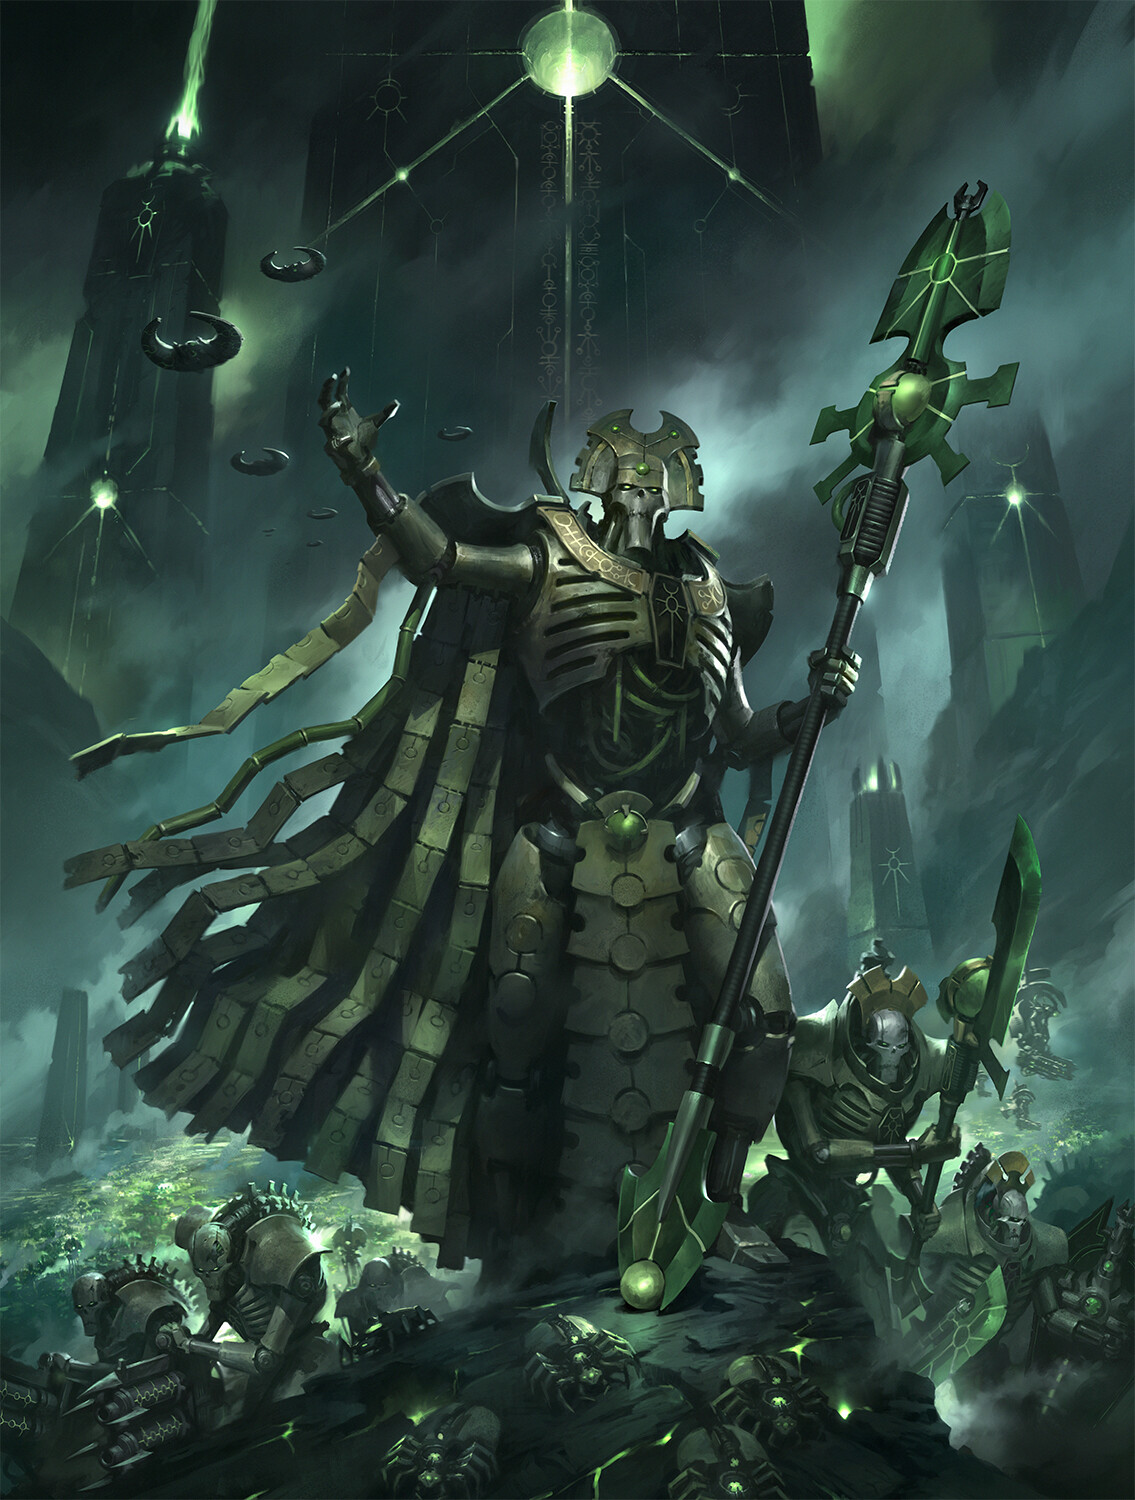
\includegraphics[height=530pt, width=400pt]{hq_art.jpg}
	\subsection[Fast Attack]{\texorpdfstring{\centering\Huge Fast Attack}{Fast Attack}}
	
	\centerline{\begin{minipage}{400pt}
			\centering
			See, Obyron, the separatists come – attempting to outflank me just as they did at the Fourth Battle of Vyndakh. How they calculate that daubing themselves green and roaring like savages will produce a different outcome, I cannot fathom; but it is of no account. Ready my legions – another glorious victory shall soon be ours.
			
			\vspace*{1em}
			\raggedleft Nemesor Zandrekh
	\end{minipage}}
}


\newpage
\clearbackground
\subsubsection[Canoptek Acanthrite Vanguard]{}
\fbox{\begin{imgminipage}{marble.jpg}[t]{0.2\textwidth}
		\color{white}
		\centering {\large FAST ATTACK}
		
		\color{black}
\end{imgminipage}}
\hspace{0.5em}
\begin{minipage}[t]{0.72\textwidth}
	{\large \textbf{Canoptek Acanthrite Vanguard \dotfill X Points}}
	
	\begin{tabular}{m{165 pt} *{10}{c}}
		& M & WS & BS & S & T & W & I & A & Ld & Sv \\
		\hline
		Canoptek Acanthrite & 12 & 4 & 4 & 4 & 5 & 3 & 2 & 2 & 10 & 3+ \\
	\end{tabular}
	\small
	\begin{minipage}[t]{0.5\textwidth}
		\begin{flushleft}
			\vspace*{2em}
			\textbf{Unit Composition}
			\begin{itemize}
				\item 3 Canoptek Acanthrites
			\end{itemize}
			
			\textbf{Wargear}
			\begin{itemize}
				\item \quickref{Cutting Beam}
				\item \quickref{Voidblade}
			\end{itemize}
		\end{flushleft}
	\end{minipage}
	\begin{minipage}[t]{0.5\textwidth}
		\begin{flushleft}
			\vspace*{2em}
			\textbf{Unit Type}
			\begin{itemize}
				\item Infantry (Canoptek, Floating, Light, \quickref{Living Metal})
			\end{itemize}
			
			\textbf{Special Rules}
			\begin{itemize}
				\item \quickref{Annihilation Protocols}
				\item \quickref{Awakening Protocols} (Silver)
				\item Bulky (2)
				\item \quickref{Reanimation Protocols}
				\item Shadowed Wings
				\item \quickref{Soulless Hordes} (Bronze)
			\end{itemize}
		\end{flushleft}
	\end{minipage}
	
	\vspace*{2em}
	\textbf{Weapons}
	
	\begin{tabular}{m{95 pt} *{4}{c} >{\raggedright\arraybackslash}p{130pt}}
		& Range & Type & S & AP & Abilities \\
		Cutting Beam & 12" & Assault 1 & 6 & 2 & Armourbane (Melta) \\
		\quickref{Voidblade} & — & Melee & User & 4 & \quickref{Entropic Strike} (4+), Rending(6+) \\
	\end{tabular}
	
	\vspace*{2em}
	\textbf{Unit Rules}
	
	\textit{Shadowed Wings}: Canoptek Acanthrites increase Shrouded saves by +1. If the model does not already have one, it instead gains Shrouded (6+).
		
	\vspace*{2em}
	\textbf{Options}
	\begin{itemize}
		\item The Canoptek Acanthrites Vanguard may include:
		\begin{itemize}
			\item Up to an additional 6 Canoptek Acanthrites \dotfill X points each
		\end{itemize}
	\end{itemize}
\end{minipage}


\newpage
\subsubsection[Canoptek Scarab Swarms]{}

\begin{minipage}[t]{0.72\textwidth}
	{\large \textbf{Canoptek Scarab Swarms \dotfill X Points}}
	
	\begin{tabular}{m{165 pt} *{10}{c}}
		& M & WS & BS & S & T & W & I & A & Ld & Sv \\
		\hline
		Canoptek Scarab Swarm & 10 & 2 & 2 & 3 & 3 & 3 & 2 & 4 & 10 & 6+ \\
	\end{tabular}
	\small
	\begin{minipage}[t]{0.5\textwidth}
		\begin{flushleft}
			\vspace*{2em}
			\textbf{Unit Composition}
			\begin{itemize}
				\item 3 Canoptek Scarab Swarms
			\end{itemize}
			
			\textbf{Wargear}
			\begin{itemize}
				\item Feeder Mandibles
			\end{itemize}
		\end{flushleft}
	\end{minipage}
	\begin{minipage}[t]{0.5\textwidth}
		\begin{flushleft}
			\vspace*{2em}
			\textbf{Unit Type}
			\begin{itemize}
				\item Infantry (Canoptek, Floating, Light, \quickref{Living Metal})
			\end{itemize}
			
			\textbf{Special Rules}
			\begin{itemize}
				\item \quickref{Reanimation Protocols}
				\item \quickref{Soulless Hordes} (Bronze)
				\item Swarms
			\end{itemize}
		\end{flushleft}
	\end{minipage}
	
	\vspace*{2em}
	\textbf{Weapons}
	
	\begin{tabular}{m{95 pt} *{4}{c} >{\raggedright\arraybackslash}p{130pt}}
		& Range & Type & S & AP & Abilities \\
		Feeder Mandible & — & Melee & User & — & \quickref{Entropic Strike} (4+) \\
	\end{tabular}

	\vspace*{2em}
	\textbf{Options}
	\begin{itemize}
		\item The Canoptek Scarab Swarms may include:
		\begin{itemize}
			\item Up to an additional 6 Canoptek Scarab Swarm models \dotfill X points each
		\end{itemize}
	\end{itemize}
\end{minipage}
\hspace{0.5em}
\fbox{\begin{imgminipage}{marble.jpg}[t]{0.2\textwidth}
	\color{white}
	\centering {\large FAST ATTACK}
	
	\color{black}
\end{imgminipage}}


\newpage
\subsubsection[Canoptek Spyder Cohort]{}
\fbox{\begin{imgminipage}{marble.jpg}[t]{0.2\textwidth}
		\color{white}
		\centering {\large FAST ATTACK}
		
		\color{black}
\end{imgminipage}}
\hspace{0.5em}
\begin{minipage}[t]{0.72\textwidth}
	{\large \textbf{Canoptek Spyder Cohort \dotfill X Points}}
	
	\begin{tabular}{m{165 pt} *{10}{c}}
		& M & WS & BS & S & T & W & I & A & Ld & Sv \\
		\hline
		Canoptek Spyder & 7 & 3 & 3 & 6 & 6 & 3 & 2 & 1 & 10 & 3+ \\
	\end{tabular}
	\small
	\begin{minipage}[t]{0.5\textwidth}
		\begin{flushleft}
			\vspace*{2em}
			\textbf{Unit Composition}
			\begin{itemize}
				\item 1 Canoptek Spyder
			\end{itemize}
			
			\textbf{Wargear}
			\begin{itemize}
				\item Close Combat Weapon
			\end{itemize}
		\end{flushleft}
	\end{minipage}
	\begin{minipage}[t]{0.5\textwidth}
		\begin{flushleft}
			\vspace*{2em}
			\textbf{Unit Type}
			\begin{itemize}
				\item Infantry (Canoptek, Floating, \quickref{Living Metal})
			\end{itemize}
			
			\textbf{Special Rules}
			\begin{itemize}
				\item Bulky (2)
				\item \quickref{Reanimation Protocols}
				\item Nodal Relay
				\item Relentless
				\item Scarab Hive
				\item \quickref{Soulless Hordes} (Silver)
			\end{itemize}
		\end{flushleft}
	\end{minipage}
	
	\vspace*{2em}
	\textbf{Weapons}
	
	\begin{tabular}{m{95 pt} *{4}{c} >{\raggedright\arraybackslash}p{130pt}}
		& Range & Type & S & AP & Abilities \\
		Fabricator Claw Array & — & Melee & User & 5 & — \\
		\quickref{Particle Beamer} & 24" & Heavy 1 & 6 & 5 & Blast, Twin-Linked \\
	\end{tabular}
	
	\vspace*{2em}
	\textbf{Unit Rules}
	
	\textit{Fabricator Claw Array:} Each model with a Fabricator Claw Array gains the Battlesmith (4+) special rule.
	
	\textit{Nodal Relay:} If a Canoptek Spyder is within \quickref{Nodal Range} of a model it will extend that range an additional 6" from the Spyder model, acting as a relay point.
	
	\textit{Scarab Hive:} Once per friendly Movement phase, each Canoptek Spyder model can use this special rule to create Canoptek Scarab Swarms. To do so, nominate a friendly unit of Canoptek Scarab Swarms that is within 6" of the Canoptek Spyder. Add a single Canoptek Scarab Swarm base to the unit – this can take the unit beyond its starting size, but must be placed within 6" of the Canoptek Spyder. If a model cannot be placed for any reason, it is destroyed. Canoptek Scarab Swarms created in this manner can move and act normally this turn. Roll a D6 each time a Canoptek Spyder uses its Scarab Hive special rule, immediately after placing any Canoptek Scarab Swarms that were created – on a roll of a 1 the Canoptek Spyder suffers a single Wound with no saves of any kind allowed. In addition, for each Canoptek Spyder Cohort in the army, a unit of Canoptek Scarab Swarms may be taken which do count towards the maximum number of units in their respective Force Organisation slot.
	
	
	\vspace*{2em}
	\textbf{Options}
	\begin{itemize}
		\item The Canoptek Spyder Cohort may include:
		\begin{itemize}
			\item Up to an additional 2 Canoptek Spyders \dotfill X points each
		\end{itemize}
		\item Each model may take replace their Close Combat Weapon with a:
		\begin{itemize}
			\item Fabricator Claw Array \dotfill X points each
		\end{itemize}
		\item Each model may take any of the following options:
		\begin{itemize}
		\item \quickref{Gloom Prism} \dotfill X points each
		\item Twin-Linked \quickref{Particle Beamer} \dotfill X points each
		\end{itemize}
	\end{itemize}
\end{minipage}


\newpage
\subsubsection[Canoptek Tomb Sentinel]{}
\begin{minipage}[t]{0.72\textwidth}
	{\large \textbf{Canoptek Tomb Sentinel \dotfill X Points}}
	
	\begin{tabular}{m{165 pt} *{10}{c}}
		& M & WS & BS & S & T & W & I & A & Ld & Sv \\
		\hline
		Canoptek Tomb Sentinel & 10 & 3 & 3 & 6 & 7 & 4 & 2 & 2 & 10 & 3+ \\
	\end{tabular}
	\small
	\begin{minipage}[t]{0.5\textwidth}
		\begin{flushleft}
			\vspace*{2em}
			\textbf{Unit Composition}
			\begin{itemize}
				\item 1 Canoptek Tomb Sentinel
			\end{itemize}
			
			\textbf{Wargear}
			\begin{itemize}
				\item Close Combat Weapon
				\item \quickref{Exile Cannon}
			\end{itemize}
		\end{flushleft}
	\end{minipage}
	\begin{minipage}[t]{0.5\textwidth}
		\begin{flushleft}
			\vspace*{2em}
			\textbf{Unit Type}
			\begin{itemize}
				\item Infantry (Canoptek, \quickref{Living Metal}, Monstrous)
			\end{itemize}
			
			\textbf{Special Rules}
			\begin{itemize}
				\item Bulky (3)
				\item Outflank
				\item Phase Generator
				\item Phase Tunelling
				\item Rampage (1)
				\item \quickref{Reanimation Protocols}
				\item Sense Clusters
				\item \quickref{Soulles Hordes} (Silver)
				\item Subterranean Assault
				\item \quickref{Tomb Guardians}
			\end{itemize}
		\end{flushleft}
	\end{minipage}
	
	\vspace*{2em}
	\textbf{Weapons}
	
	\begin{tabular}{m{95 pt} *{4}{c} >{\raggedright\arraybackslash}p{130pt}}
		& Range & Type & S & AP & Abilities \\
		\quickref{Exile Cannon} & 12" & Heavy 1 & 10 & 2 & Blast, \quickref{Exile Ray} (5+), Ignores Cover \\
	\end{tabular}
	
	\vspace*{2em}
	\textbf{Unit Rules}
	
	\textit{Phase Generator:} The Canoptek Tomb Sentinel has a 4+ invulnerable save.
	
	\textit{Phase Tunelling:} When moving, a Canoptek Tomb Sentinel can move over all other models and terrain as if they were open ground. However, it cannot end their move on top of other models and can only end their move on top of impassable terrain if it is possible to actually place the models on top of it.
	
	\textit{Scarab Hive:} A Canoptek Tomb Stalker is immune to Blind and has the Night Vision special rule.	
	
	\vspace*{2em}
	\textbf{Options}
	\begin{itemize}
		\item The Canoptek Tomb Stalker may take any of the following options:
		\begin{itemize}
			\item \quickref{Gloom Prism} \dotfill X points each
			\item \quickref{Sepulchral Scarabs} \dotfill X points each
		\end{itemize}
	\end{itemize}
\end{minipage}
\hspace{0.5em}
\fbox{\begin{imgminipage}{marble.jpg}[t]{0.2\textwidth}
	\color{white}
	\centering {\large FAST ATTACK}
	
	\color{black}
\end{imgminipage}}


\newpage
\subsubsection[Canoptek Tomb Stalker]{}

\fbox{\begin{imgminipage}{marble.jpg}[t]{0.2\textwidth}
		\color{white}
		\centering {\large FAST ATTACK}
		
		\color{black}
\end{imgminipage}}
\hspace{0.5em}
\begin{minipage}[t]{0.72\textwidth}
	{\large \textbf{Canoptek Tomb Stalker \dotfill X Points}}
	
	\begin{tabular}{m{165 pt} *{10}{c}}
		& M & WS & BS & S & T & W & I & A & Ld & Sv \\
		\hline
		Canoptek Tomb Stalker & 10 & 3 & 3 & 6 & 7 & 4 & 2 & 4 & 10 & 3+ \\
	\end{tabular}
	\small
	\begin{minipage}[t]{0.5\textwidth}
		\begin{flushleft}
			\vspace*{2em}
			\textbf{Unit Composition}
			\begin{itemize}
				\item 1 Canoptek Tomb Stalker
			\end{itemize}
			
			\textbf{Wargear}
			\begin{itemize}
				\item Two Close Combat Weapons
				\item Two \quickref{Gauss Flayer}s
			\end{itemize}
		\end{flushleft}
	\end{minipage}
	\begin{minipage}[t]{0.5\textwidth}
		\begin{flushleft}
			\vspace*{2em}
			\textbf{Unit Type}
			\begin{itemize}
				\item Infantry (Canoptek, Light, \quickref{Living Metal}, Monstrous)
			\end{itemize}
			
			\textbf{Special Rules}
			\begin{itemize}
				\item Bulky (3)
				\item Firing Protocols (2)
				\item Outflank
				\item Phase Generator
				\item Phase Tunelling
				\item Rampage (1)
				\item \quickref{Reanimation Protocols}
				\item Sense Clusters
				\item \quickref{Soulles Hordes} (Silver)
				\item Subterranean Assault
				\item \quickref{Tomb Guardians}
			\end{itemize}
		\end{flushleft}
	\end{minipage}
	
	\vspace*{2em}
	\textbf{Weapons}
	
	\begin{tabular}{m{95 pt} *{4}{c} >{\raggedright\arraybackslash}p{130pt}}
		& Range & Type & S & AP & Abilities \\
		\quickref{Gauss Flayer} & 24" & Rapid Fire & 4 & 5 & \quickref{Gauss} (6+) \\
	\end{tabular}
	
	\vspace*{2em}
	\textbf{Unit Rules}
	
	\textit{Phase Generator:} The Canoptek Tomb Sentinel has a 4+ invulnerable save.
	
	\textit{Phase Tunelling:} When moving, a Canoptek Tomb Sentinel can move over all other models and terrain as if they were open ground. However, it cannot end their move on top of other models and can only end their move on top of impassable terrain if it is possible to actually place the models on top of it.
	
	\textit{Scarab Hive:} A Canoptek Tomb Stalker is immune to Blind and has the Night Vision special rule.	
	
	\vspace*{2em}
	\textbf{Options}
	\begin{itemize}
		\item The Canoptek Tomb Stalker may take any of the following options:
		\begin{itemize}
			\item \quickref{Gloom Prism} \dotfill X points each
			\item \quickref{Sepulchral Scarabs} \dotfill X points each
		\end{itemize}
	\end{itemize}
\end{minipage}




\newpage
\subsubsection[Canoptek Wraith Flight]{}

\fbox{\begin{imgminipage}{marble.jpg}[t]{0.2\textwidth}
		\color{white}
		\centering {\large FAST ATTACK}
		
		\color{black}
\end{imgminipage}}
\hspace{0.5em}
\begin{minipage}[t]{0.72\textwidth}
	{\large \textbf{Canoptek Wraith Flight \dotfill X Points}}
	
	\begin{tabular}{m{165 pt} *{10}{c}}
		& M & WS & BS & S & T & W & I & A & Ld & Sv \\
		\hline
		Canoptek Wraith & 12 & 3 & 3 & 4 & 5 & 2 & 2 & 3 & 10 & 3+ \\
	\end{tabular}
	\small
	\begin{minipage}[t]{0.5\textwidth}
		\begin{flushleft}
			\vspace*{2em}
			\textbf{Unit Composition}
			\begin{itemize}
				\item 3 Canoptek Wraiths
			\end{itemize}
			
			\textbf{Wargear}
			\begin{itemize}
				\item Close Combat Weapon
			\end{itemize}
		\end{flushleft}
	\end{minipage}
	\begin{minipage}[t]{0.5\textwidth}
		\begin{flushleft}
			\vspace*{2em}
			\textbf{Unit Type}
			\begin{itemize}
				\item Infantry (Canoptek, Light, \quickref{Living Metal})
			\end{itemize}
			
			\textbf{Special Rules}
			\begin{itemize}
				\item Bulky (3)
				\item \quickref{Reanimation Protocols}
				\item \quickref{Soulless Hordes} (Silver)
				\item Wraithform
				\item Wraithflight
			\end{itemize}
		\end{flushleft}
	\end{minipage}
	
	\vspace*{2em}
	\textbf{Weapons}
	
	\begin{tabular}{m{95 pt} *{4}{c} >{\raggedright\arraybackslash}p{130pt}}
		& Range & Type & S & AP & Abilities \\
		\quickref{Whip Coils} & — & Melee & User & — & Reach (3) \\
		\quickref{Particle Caster} & 12" & Pistol 1 & 6 & 5 & — \\
		\quickref{Transdimensional Beamer} & 12" & Heavy 1 & 4 & 5 & \quickref{Exile Ray} (6+) \\
	\end{tabular}
	
	\vspace*{2em}
	\textbf{Unit Rules}
	
	\textit{Wraithform:} Each Canoptek Wraith has a 3+ invulnerable save.
	
	\textit{Wraithflight:} When moving, a Canoptek Wraith can move over all other models and terrain as if they were open ground. However, it cannot end their move on top of other models and can only end their move on top of impassable terrain if it is possible to actually place the models on top of it.	
	
	\vspace*{2em}
	\textbf{Options}
	\begin{itemize}
		\item The Canoptek Wraith Flight may include:
		\begin{itemize}
			\item Up to an additional 3 Canoptek Wraiths \dotfill X points each
		\end{itemize}
		\item Each model may take exchange their Close Combat Weapon for:
		\begin{itemize}
			\item \quickref{Whip Coils} \dotfill X points each
		\end{itemize}
		\item Each model may take one of the following options:
		\begin{itemize}
			\item \quickref{Particle Caster} \dotfill X points each
			\item \quickref{Transdimensional Beamer} \dotfill X points each
		\end{itemize}
	\end{itemize}
\end{minipage}


\newpage
\subsubsection[Ghost Ark]{}
\fbox{\begin{imgminipage}{marble.jpg}[t]{0.2\textwidth}
		\color{white}
		\centering {\large Fast Attack}
		
		\raggedright \small
		\color{black}
\end{imgminipage}}
\hspace{0.5em}
\begin{minipage}[t]{0.72\textwidth}
	{\large \textbf{Ghost Ark \dotfill X Points}}
	\begin{NiceTabular}{m{145 pt} *{2}{c} | *{3}{c} | c | c }
		& & & \cellgray{3}{Armour} & & & & \cellgray{1}{Transport} \\
		& M & BS & \cellgray{1}{Front} & \cellgray{1}{Side} & \cellgray{1}{Rear} & HP & \cellgray{1}{Capacity} \\
		\hline
		Ghost Ark & 12 & 4 & \cellgray{1}{11} & \cellgray{1}{11} & \cellgray{1}{11} & 4 &\cellgray{1}{11} \\
	\end{NiceTabular}
	\small
	\begin{minipage}[t]{0.5\textwidth}
		\begin{flushleft}
			\vspace*{2em}
			\textbf{Unit Composition}
			\begin{itemize}
				\item 1 Ghost Ark
			\end{itemize}
			
			\textbf{Wargear}
			\begin{itemize}
				\item Five Sponson (Left) Mounted \quickref{Gauss Flayer}s
				\item Five Sponson (Right) Mounted \quickref{Gauss Flayer}s
				\item \quickref{Quantum Shielding}
			\end{itemize}
		\end{flushleft}
	\end{minipage}
	\begin{minipage}[t]{0.5\textwidth}
		\begin{flushleft}
			\vspace*{2em}
			\textbf{Unit Type}
			\begin{itemize}
				\item Vehicle (\quickref{Living Metal}, Open-Topped, Skimmer, Transport)
			\end{itemize}
			
			\textbf{Special Rules}
			\begin{itemize}
				\item \quickref{Awakening Protocols} (Bronze)
				\item Power of the Machine Spirit
			\end{itemize}
		\end{flushleft}
	\end{minipage}

	\vspace*{2em}
	\textbf{Access Points}
	
	The Ghost Ark has three Access Points on the Front and Sides of the hull.
	
	\vspace*{2em}
	\textbf{Weapons}
	
	\begin{tabular}{m{95 pt} *{4}{c} >{\raggedright\arraybackslash}p{130pt}}
		& Range & Type & S & AP & Abilities \\
		\hline
		\quickref{Gauss Flayer} & 24" & Rapid Fire & 4 & 5 & \quickref{Gauss} (6+) \\
	\end{tabular}
	
	\vspace*{2em}
	\textbf{Unit Rules}
	
	\textit{Repair Barge}: At the start of each friendly Movement phase, this model can repair fallen Dynastic Warriors. To do so, nominate a friendly unit of Dynastic Warriors that is either within 6" of this model or embarked upon it, and roll a D3: that unit reanimate that may times; if embarked, this cannot return models above the Transport Capacity. These Dynastic Warriors must be placed within 6" of the Ghost Ark, or if the unit is currently embarked in the Ghost Ark, within it. If a model cannot be placed for any reason, it is destroyed. Dynastic Warriors repaired in this manner can move and act normally this turn. 
	
	
	\vspace*{2em}
	\textbf{Options}
	\begin{itemize}
	\item A Ghost Ark may take:
	\begin{itemize}
		\item \quickref{Quantum Shielding Matrix} \dotfill X points
	\end{itemize} 
	\end{itemize} 
\end{minipage}



\newpage
\subsubsection[Night Scythe]{}
\fbox{\begin{imgminipage}{marble.jpg}[t]{0.2\textwidth}
		\color{white}
		\centering {\large Fast Attack}
		
		\raggedright \small
		\color{black}
\end{imgminipage}}
\hspace{0.5em}
\begin{minipage}[t]{0.72\textwidth}
	{\large \textbf{Night Scythe \dotfill X Points}}
	\begin{NiceTabular}{m{145 pt} *{2}{c} | *{3}{c} | c | c }
		& & & \cellgray{3}{Armour} & & & & \cellgray{1}{Transport} \\
		& M & BS & \cellgray{1}{Front} & \cellgray{1}{Side} & \cellgray{1}{Rear} & HP & \cellgray{1}{Capacity} \\
		\hline
		Night Scythe & 24 & 4 & \cellgray{1}{11} & \cellgray{1}{11} & \cellgray{1}{11} & 4 &\cellgray{1}{—} \\
	\end{NiceTabular}
	\small
	\begin{minipage}[t]{0.5\textwidth}
		\begin{flushleft}
			\vspace*{2em}
			\textbf{Unit Composition}
			\begin{itemize}
				\item 1 Night Scythe
			\end{itemize}
			
			\textbf{Wargear}
			\begin{itemize}
				\item Hull (Front) Mounted Twin-Lined \quickref{Tesla Destrucor}
				\item Captive Wormhole
			\end{itemize}
		\end{flushleft}
	\end{minipage}
	\begin{minipage}[t]{0.5\textwidth}
		\begin{flushleft}
			\vspace*{2em}
			\textbf{Unit Type}
			\begin{itemize}
				\item Vehicle (Hover, Flyer, \quickref{Living Metal}, Transport)
			\end{itemize}
			
			\textbf{Special Rules}
			\begin{itemize}
				\item \quickref{Awakening Protocols} (Bronze)
				\item Invasion Beams
			\end{itemize}
		\end{flushleft}
	\end{minipage}
	
	\vspace*{2em}
	\textbf{Access Points}
	
	The Night Scythe has one Access Point on each side of the hull.
	
	\vspace*{2em}
	\textbf{Weapons}
	
	\begin{tabular}{m{95 pt} *{4}{c} >{\raggedright\arraybackslash}p{130pt}}
		& Range & Type & S & AP & Abilities \\
		\hline
		\quickref{Tesla Destructor} & 24" & Heavy 4 & 7 & — & \quickref{Tesla} (6+), Twin-Linked
	\end{tabular}
	
	\vspace*{2em}
	\textbf{Unit Rules}
	
	\textit{Captive Wormhole:} A Night Scythe does not have a Transport Capacity. Instead, units embarked on the it are stationed at its Captive Wormhole. The stationed unit may exit the Night Scythe using any of the normal Transport rule, however they are never affected by anything that affects Passengers and do not count as being embarked for the purposes of special rules. While the unit is stationed at the Captive Wormhole, they also count as being in \quickref{Teleportation Reserve}; should the Night Scythe be destroyed, the prepared unit is not affected and goes into \quickref{Teleportation Reserve}. A unit that embark the Night Scythe are sent to the Captive Wormhole and count as being stationed at the Captive Wormhole. A Night Scythe can only have a single unit stationed at its Captive Wormhole at any given time.
	
	\textit{Invasion Beams}: A unit that begins its Movement phase embarked upon a Night Scythe can disembark either before or after it has moved (including pivoting on the spot), even though it is Zooming, so long it has not moved more than 36" in that Movement phase. If a unit disembarks from a Night Scythe after it has moved 24" or more, models in the unit can only fire Snap Shots until the start of their next turn.
\end{minipage}


\newpage
\subsubsection[Tomb Blade Wing]{}

\fbox{\begin{imgminipage}{marble.jpg}[t]{0.2\textwidth}
		\color{white}
		\centering {\large FAST ATTACK}
		
		\color{black}
\end{imgminipage}}
\hspace{0.5em}
\begin{minipage}[t]{0.72\textwidth}
	{\large \textbf{Tomb Blade Wing \dotfill X Points}}
	
	\begin{tabular}{m{165 pt} *{10}{c}}
		& M & WS & BS & S & T & W & I & A & Ld & Sv \\
		\hline
		Tomb Blade & 16 & 4 & 4 & 4 & 5 & 2 & 2 & 1 & 10 & 4+ \\
	\end{tabular}
	\small
	\begin{minipage}[t]{0.5\textwidth}
		\begin{flushleft}
			\vspace*{2em}
			\textbf{Unit Composition}
			\begin{itemize}
				\item 3 Tomb Blades
			\end{itemize}
			
			\textbf{Wargear}
			\begin{itemize}
				\item Twin-Linked \quickref{Gauss Blaster}
			\end{itemize}
		\end{flushleft}
	\end{minipage}
	\begin{minipage}[t]{0.5\textwidth}
		\begin{flushleft}
			\vspace*{2em}
			\textbf{Unit Type}
			\begin{itemize}
				\item Cavalry (Floating, \quickref{Living Metal}, Skirmish)
			\end{itemize}
			
			\textbf{Special Rules}
			\begin{itemize}
				\item \quickref{Awakening Protocols} (Silver)
				\item Bulky (3)
				\item Hammer of Wrath (1)
				\item Hit \& Run
				\item Outflank
				\item \quickref{Reanimation Protocols}
				\item Relentless
			\end{itemize}
		\end{flushleft}
	\end{minipage}
	
	\vspace*{2em}
	\textbf{Weapons}
	
	\begin{tabular}{m{95 pt} *{4}{c} >{\raggedright\arraybackslash}p{130pt}}
		& Range & Type & S & AP & Abilities \\
		\quickref{Gauss Blaster} & 24" & Rapid Fire & 5 & 4 & \quickref{Gauss} (6+), Twin-Linked \\
		\quickref{Tesla Carbine} & 24" & Assault 2 & 5 & — & \quickref{Tesla} (6+), Twin-Linked \\
		\quickref{Particle Beamer} & 24" & Heavy 1 & 6 & 5 & Blast \\
	\end{tabular}
	
	\vspace*{2em}
	\textbf{Unit Rules}
	
	\textit{Nebuloscope}: A model with a Nebuloscope gains the Night Vision special rule and their weapons gain the Ignores Cover special rule.
	
	\textit{Shadowloom}: A model with a Shadowloom increases Shrouded saves by +1. If it does not already have one, it instead gains Shrouded (6+).
	
	\textit{Shieldvane}: A model with a Shieldvane increases their save to 3+.
	
	\vspace*{2em}
	\textbf{Options}
	\begin{itemize}
		\item The Tomb Blade Wing may include:
		\begin{itemize}
			\item Up to an additional 7 Tomb Blades \dotfill X points each
		\end{itemize}
		\item Each Tomb Blade make take any of the following options:
		\begin{itemize}
			\item \quickref{Nebuloscope} \dotfill X points each
			\item \quickref{Shadowloom} \dotfill X points each
			\item \quickref{Shieldvane} \dotfill X points each
		\end{itemize}
		\item Each Tomb Blade may exchange their Twin-Linked \quickref{Gauss Blaster} for one of the following:
		\begin{itemize}
			\item Twin-Linked \quickref{Tesla Carbine} \dotfill X points each
			\item \quickref{Particle Beamer} \dotfill X points each
		\end{itemize}
	\end{itemize}
\end{minipage}
	
	\newpage
	\setbackground
{
	\centering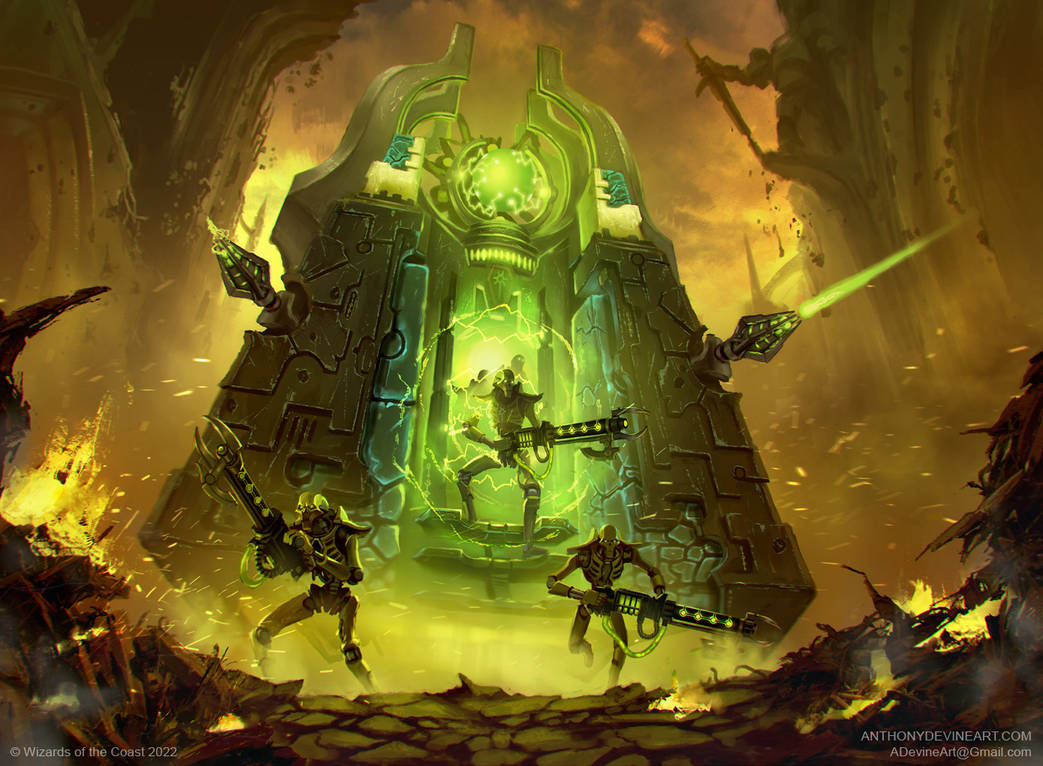
\includegraphics[height=400pt, width=400pt]{heavy_art.jpg}
	\subsection{\texorpdfstring{\centering\Huge Heavy Support}{Heavy Support}}
	
	\centerline{\begin{minipage}{400pt}
			\centering
			"We thought in terms of wars. Of destruction. Of conquest. But eternity also requires what you would call...entertainment."
			
			\vspace*{1em}
			\raggedleft Djoseras
	\end{minipage}}
}

\newpage
\clearbackground
\subsubsection[Canoptek Doomstalker Patrol]{}

\fbox{\begin{imgminipage}{marble.jpg}[t]{0.2\textwidth}
		\color{white}
		\centering {\large HEAVY SUPPORT}
		
		\color{black}
\end{imgminipage}}
\hspace{0.5em}
\begin{minipage}[t]{0.72\textwidth}
	{\large \textbf{Canoptek Doomstalker Patrol \dotfill X Points}}
	
	\begin{tabular}{m{165 pt} *{10}{c}}
		& M & WS & BS & S & T & W & I & A & Ld & Sv \\
		\hline
		Canoptek Doomstalker & 10 & 3 & 3 & 6 & 6 & 6 & 2 & 3 & 10 & 3+ \\
	\end{tabular}
	\small
	\begin{minipage}[t]{0.5\textwidth}
		\begin{flushleft}
			\vspace*{2em}
			\textbf{Unit Composition}
			\begin{itemize}
				\item 1 Canoptek Doomstalker
			\end{itemize}
			
			\textbf{Wargear}
			\begin{itemize}
				\item Close Combat Weapon
				\item \quickref{Doomsday Blaster}
				\item Two \quickref{Gauss Flayer}s
			\end{itemize}
		\end{flushleft}
	\end{minipage}
	\begin{minipage}[t]{0.5\textwidth}
		\begin{flushleft}
			\vspace*{2em}
			\textbf{Unit Type}
			\begin{itemize}
				\item Dreadnought (Canoptek, \quickref{Living Metal})
			\end{itemize}
			
			\textbf{Special Rules}
			\begin{itemize}
				\item Containment Field
				\item \quickref{Reanimation Protocols}
				\item Sentinel Protocols
				\item \quickref{Soulles Hordes} (Silver)
			\end{itemize}
		\end{flushleft}
	\end{minipage}
	
	\vspace*{2em}
	\textbf{Weapons}
	
	\begin{tabular}{m{95 pt} *{4}{c} >{\raggedright\arraybackslash}p{130pt}}
		& Range & Type & S & AP & Abilities \\
		\quickref{Doomsday Blaster} & & & & & \\
		— Low Power & 24" & Heavy 1 & 8 & 3 & Blast \\
		— High Power & 48" & Heavy 1 & 10 & 1 & Large Blast, Divert Power \\
		\quickref{Gauss Flayer} & 24" & Rapid Fire & 4 & 5 & \quickref{Gauss} (6+) \\
	\end{tabular}
	
	\vspace*{2em}
	\textbf{Unit Rules}
	
	\textit{Containment Field:} Canoptek Doomstalker models have a 4+ Invulnerable Save and any model with an containment field and a Wounds Characteristic that suffers an unsaved Wound with the Instant Death special rule is not immediately removed as a casualty, but instead loses D3 Wounds instead of one for each unsaved Wound with the Instant Death special rule inflicted on it. In addition, when a model with an containment field loses its last Wound or Hull Point, but before it is removed as a casualty or replaced with a Wreck, all models both friendly and enemy within D6" suffer an automatic Hit at Str 8, AP —. 
	
	\textit{Sentinel Protocols:} %TODO: This
	
	\vspace*{2em}
	\textbf{Options}
	\begin{itemize}
		\item The Canoptek Doomstalker Patrol may include:
		\begin{itemize}
			\item Up to an additional 1 Canoptek Doomstalker \dotfill X points each
		\end{itemize}
	\end{itemize}
\end{minipage}



\newpage
\subsubsection[Doomsday Ark]{}
\fbox{\begin{imgminipage}{marble.jpg}[t]{0.2\textwidth}
		\color{white}
		\centering {\large HEAVY SUPPORT}
		
		\raggedright \small
		\color{black}
\end{imgminipage}}
\hspace{0.5em}
\begin{minipage}[t]{0.72\textwidth}
	{\large \textbf{Doomsday Ark \dotfill X Points}}
	\begin{NiceTabular}{m{145 pt} *{2}{c} | *{3}{c} | c | c }
		& & & \cellgray{3}{Armour} & & & & \cellgray{1}{Transport} \\
		& M & BS & \cellgray{1}{Front} & \cellgray{1}{Side} & \cellgray{1}{Rear} & HP & \cellgray{1}{Capacity} \\
		\hline
		Doomsday Ark & 12 & 4 & \cellgray{1}{11} & \cellgray{1}{11} & \cellgray{1}{11} & 4 &\cellgray{1}{—} \\
	\end{NiceTabular}
	\small
	\begin{minipage}[t]{0.5\textwidth}
		\begin{flushleft}
			\vspace*{2em}
			\textbf{Unit Composition}
			\begin{itemize}
				\item 1 Doomsday Ark
			\end{itemize}
			
			\textbf{Wargear}
			\begin{itemize}
				\item Hull (Front) Mounted \quickref{Doomsday Cannon}
				\item Five Sponson (Left) Mounted \quickref{Gauss Flayer}s
				\item Five Sponson (Right) Mounted \quickref{Gauss Flayer}s
				\item \quickref{Quantum Shielding}
			\end{itemize}
		\end{flushleft}
	\end{minipage}
	\begin{minipage}[t]{0.5\textwidth}
		\begin{flushleft}
			\vspace*{2em}
			\textbf{Unit Type}
			\begin{itemize}
				\item Vehicle (\quickref{Living Metal}, Open-Topped Skimmer)
			\end{itemize}
			
			\textbf{Special Rules}
			\begin{itemize}
				\item \quickref{Awakening Protocols} (Silver)
				\item Power of the Machine Spirit
			\end{itemize}
		\end{flushleft}
	\end{minipage}
	
	\vspace*{2em}
	\textbf{Weapons}
	
	\begin{tabular}{m{95 pt} *{4}{c} >{\raggedright\arraybackslash}p{130pt}}
		& Range & Type & S & AP & Abilities \\
		\hline
		\quickref{Doomsday Cannon} & & & & & \\
		— Low Power & 36" & Heavy 1 & 8 & 3 & Blast \\
		— High Power & 72" & Heavy 1 & 10 & 1 & Large Blast, Divert Power \\
		\quickref{Gauss Flayer} & 24" & Rapid Fire & 4 & 5 & \quickref{Gauss} (6+) \\
	\end{tabular}


	\vspace*{2em}
	\textbf{Options}
	\begin{itemize}
	\item A Doomsday Ark may take:
	\begin{itemize}
		\item \quickref{Quantum Shielding Matrix} \dotfill X points
	\end{itemize} 
	\end{itemize} 
\end{minipage}


\newpage
\subsubsection[Doom Scythe]{}
\fbox{\begin{imgminipage}{marble.jpg}[t]{0.2\textwidth}
		\color{white}
		\centering {\large HEAVY SUPPORT}
		
		\raggedright \small
		\color{black}
\end{imgminipage}}
\hspace{0.5em}
\begin{minipage}[t]{0.72\textwidth}
	{\large \textbf{Doom Scythe \dotfill X Points}}
	\begin{NiceTabular}{m{145 pt} *{2}{c} | *{3}{c} | c | c }
		& & & \cellgray{3}{Armour} & & & & \cellgray{1}{Transport} \\
		& M & BS & \cellgray{1}{Front} & \cellgray{1}{Side} & \cellgray{1}{Rear} & HP & \cellgray{1}{Capacity} \\
		\hline
		Doom Scythe & 24 & 4 & \cellgray{1}{11} & \cellgray{1}{11} & \cellgray{1}{11} & 4 &\cellgray{1}{—} \\
	\end{NiceTabular}
	\small
	\begin{minipage}[t]{0.5\textwidth}
		\begin{flushleft}
			\vspace*{2em}
			\textbf{Unit Composition}
			\begin{itemize}
				\item 1 Doom Scythe
			\end{itemize}
			
			\textbf{Wargear}
			\begin{itemize}
				\item Hull (Front) Mounted \quickref{Heavy Death Ray}
				\item Hull (Front) Mounted Twink-Linked \quickref{Tesla Destructor}
			\end{itemize}
		\end{flushleft}
	\end{minipage}
	\begin{minipage}[t]{0.5\textwidth}
		\begin{flushleft}
			\vspace*{2em}
			\textbf{Unit Type}
			\begin{itemize}
				\item Vehicle (Hover, Flyer, \quickref{Living Metal})
			\end{itemize}
			
			\textbf{Special Rules}
			\begin{itemize}
				\item \quickref{Awakening Protocols} (Silver)
			\end{itemize}
		\end{flushleft}
	\end{minipage}
	
	
	\vspace*{2em}
	\textbf{Weapons}
	
	\begin{tabular}{m{95 pt} *{4}{c} >{\raggedright\arraybackslash}p{130pt}}
		& Range & Type & S & AP & Abilities \\
		\hline
		\quickref{Heavy Death Ray} & 24" & Heavy 1 & 10 & 1 & Blast, Lance \\
		\quickref{Tesla Destructor} & 24" & Heavy 4 & 7 & — & \quickref{Tesla} (6+), Twin-Linked \\
	\end{tabular}
\end{minipage}



\newpage
\subsubsection[Monolith]{}
\fbox{\begin{imgminipage}{marble.jpg}[t]{0.2\textwidth}
		\color{white}
		\centering {\large HEAVY SUPPORT}
		
		\raggedright \small
		\color{black}
\end{imgminipage}}
\hspace{0.5em}
\begin{minipage}[t]{0.72\textwidth}
	{\large \textbf{Monolith \dotfill X Points}}
	\begin{NiceTabular}{m{145 pt} *{2}{c} | *{3}{c} | c | c }
		& & & \cellgray{3}{Armour} & & & & \cellgray{1}{Transport} \\
		& M & BS & \cellgray{1}{Front} & \cellgray{1}{Side} & \cellgray{1}{Rear} & HP & \cellgray{1}{Capacity} \\
		\hline
		Monolith & 12 & 4 & \cellgray{1}{14} & \cellgray{1}{14} & \cellgray{1}{14} & 4 &\cellgray{1}{—} \\
	\end{NiceTabular}
	\small
	\begin{minipage}[t]{0.5\textwidth}
		\begin{flushleft}
			\vspace*{2em}
			\textbf{Unit Composition}
			\begin{itemize}
				\item 1 Monolith
			\end{itemize}
			
			\textbf{Wargear}
			\begin{itemize}
				\item \quickref{Eternity Gate}
				\item Four Hull Mounted \quickref{Gauss Flux Arcs}
				\item Turret Mounted \quickref{Particle Whip}
			\end{itemize}
		\end{flushleft}
	\end{minipage}
	\begin{minipage}[t]{0.5\textwidth}
		\begin{flushleft}
			\vspace*{2em}
			\textbf{Unit Type}
			\begin{itemize}
				\item Vehicle (\quickref{Living Metal}, Skimmer)
			\end{itemize}
			
			\textbf{Special Rules}
			\begin{itemize}
				\item \quickref{Awakening Protocols} (Silver)
				\item Deep Strike
				\item Power of the Machine Spirit
			\end{itemize}
		\end{flushleft}
	\end{minipage}

	\vspace*{2em}
	\textbf{Access Points}
	
	The Monolith has one Access Point on the Front of its hull.
		
	\vspace*{2em}
	\textbf{Weapons}
	
	\begin{tabular}{m{95 pt} *{4}{c} >{\raggedright\arraybackslash}p{130pt}}
		& Range & Type & S & AP & Abilities \\
		\hline
		\quickref{Gauss Flux Arcs} & 24" & Heavy 3 & 4 & 5 & \quickref{Gauss} (6+) \\
		\quickref{Particle Whip} & 24" & Ordnance 1 & 8 & 3 & Discriminatory, Large Blast \\
	\end{tabular}
\end{minipage}

	
	\newpage
	\setbackground
{
	\centering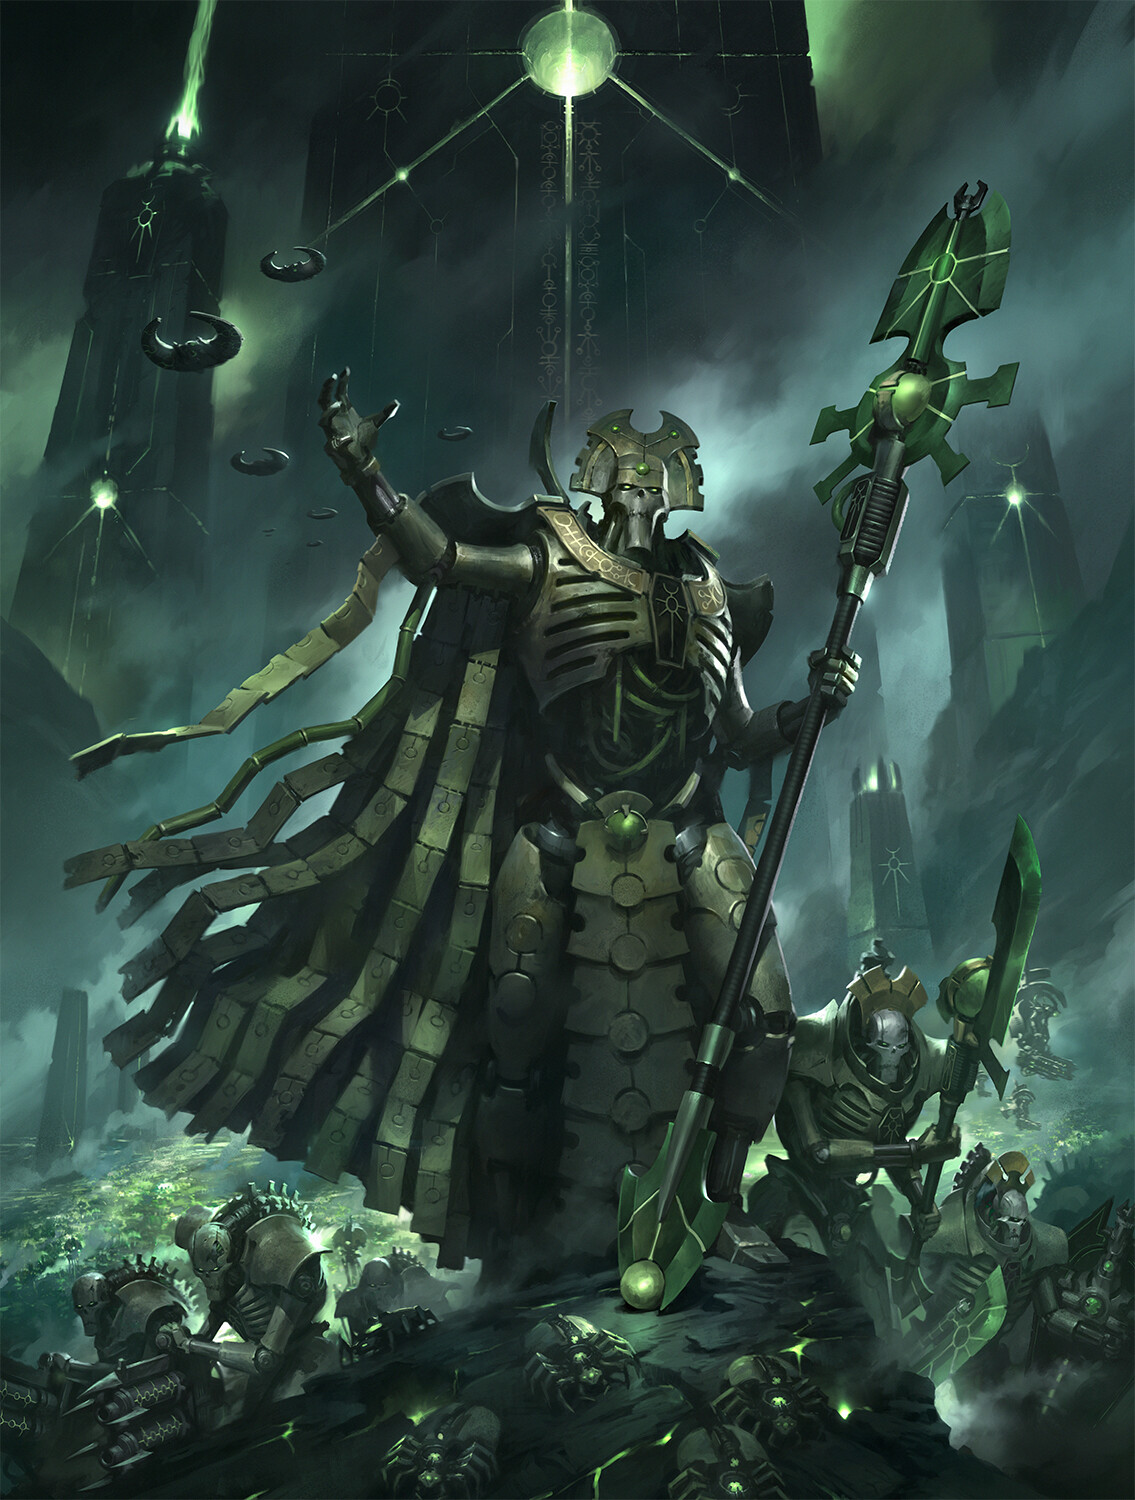
\includegraphics[height=530pt, width=400pt]{hq_art.jpg}
	\subsection[Lords of War]{\texorpdfstring{\centering\Huge Lords of War}{Lords of War}}
	
	\centerline{\begin{minipage}{400pt}
			\centering
			The silver prince nodded, and continued. ‘So, here is the lesson.’ 
			
			He extended his arm towards the far dust cloud, as if he were about to implore the oncoming Titans, still ten leagues or more away, with rhetoric. And he said one word: ‘Patience.’ 
			
			There was the tiniest, most insignificant little click. And in the same instant, the largest of the three walkers detonated, its central reactors struck dead-on by a sliver of metal moving faster than light itself. 
			
			\vspace*{1em}
			\raggedleft Djoseras
	\end{minipage}}
}

\newpage
\clearbackground
\subsubsection[Æonic Orb]{}
\fbox{\begin{imgminipage}{marble.jpg}[t]{0.2\textwidth}
		\color{white}
		\centering {\large LORDS OF WAR}
		
		\raggedright \small
		\color{black}
\end{imgminipage}}
\hspace{0.5em}
\begin{minipage}[t]{0.72\textwidth}
	{\large \textbf{Æonic Orb \dotfill X Points}}
	\begin{NiceTabular}{m{145 pt} *{2}{c} | *{3}{c} | c | c }
		& & & \cellgray{3}{Armour} & & & & \cellgray{1}{Transport} \\
		& M & BS & \cellgray{1}{Front} & \cellgray{1}{Side} & \cellgray{1}{Rear} & HP & \cellgray{1}{Capacity} \\
		\hline
		Æonic Orb & 12 & 5 & \cellgray{1}{14} & \cellgray{1}{14} & \cellgray{1}{14} & 18 &\cellgray{1}{—} \\
	\end{NiceTabular}
	\small
	\begin{minipage}[t]{0.5\textwidth}
		\begin{flushleft}
			\vspace*{2em}
			\textbf{Unit Composition}
			\begin{itemize}
				\item 1 Æonic Orb
			\end{itemize}
			
			\textbf{Wargear}
			\begin{itemize}
				\item \quickref{Quantum Shielding}
				\item \quickref{Quantum Shielding Matrix}
				\item Star Cage
			\end{itemize}
		\end{flushleft}
	\end{minipage}
	\begin{minipage}[t]{0.5\textwidth}
		\begin{flushleft}
			\vspace*{2em}
			\textbf{Unit Type}
			\begin{itemize}
				\item Super-Heavy Vehicle (\quickref{Living Metal}, Skimmer)
			\end{itemize}
			
			\textbf{Special Rules}
			\begin{itemize}
				\item Advanced Living Metal
				\item \quickref{Awakening Protocols} (Platinum)
				\item Catastrophic Destruction
				\item Power of the Machine Spirit
			\end{itemize}
		\end{flushleft}
	\end{minipage}
	
	\vspace*{2em}
	\textbf{Unit Rules}
	
	\textit{Advanced Living Metal:} This model's It Will Not Die level is increased to (1+).
	
	\vspace*{2em}
	\textbf{Weapons}
	
	\begin{tabular}{L{90 pt} c C{40pt} *{2}{c} >{\raggedright\arraybackslash}p{130pt}}
		& Range & Type & S & AP & Abilities \\
		\hline
		\quickref{Star Cage} & & & & & \\
		— Solar Burst & 72" & Destroyer 1 & 10 & 1 & Apocalyptic Blast, Blind, Ignores Cover, Lingering Death \\
		— Solar Flare & 180" & Destroyer 1 & 14 & 1 & Blind, Ignores Cover, \quickref{Path of Annihilation} (4)\\
	\end{tabular}
\end{minipage}



\newpage
\subsubsection[Doomsday Monolith]{}


\newpage
\subsubsection[Gauss Pylon]{}
% TODO: Decide here or forts

\newpage
\subsubsection[Night Shroud Bomber]{}


\newpage
\subsubsection[Sentry Pylon]{}
% TODO: Decide here or forts


\newpage
\subsubsection[Obelisk]{}


\newpage
\subsubsection[Seraptek Heavy Construct]{}
\fbox{\begin{imgminipage}{marble.jpg}[t]{0.2\textwidth}
		\color{bronze}
		\centering {\large Lords of War}
		
		\raggedright
		At the heart of many Necron tomb complexes, sleeping Seraptek Heavy Constructs await the footfall of intruders. These brutal war engines were designed by ancient Cryptek conclaves to protect each world’s master program, and this they do with merciless efficiency. Generators thrumming, the huge constructs advance with frightening speed, their optic lenses glowing as they pick out their targets. Massive cannons swivel in gimbal housings, crackling with destructive energies before unleashing pinpoint salvos to annihilate the interlopers. Should foes stray too close, the tomb guardians lash out with impaling forelimbs, their energy-sheathed tips rending metal, flesh and bone alike at a molecular level.
		
		As the legions of the Necron dynasties march out into the stars in ever-greater numbers, many Necron Overlords have summoned their Seraptek constructs to join their ranks, replacing their timeless vigils with front-line battlefield duties. In this capacity, Seraptek Heavy Constructs have proven mighty engines of conquest, more than capable of meeting an Imperial Knight or Ork Stompa head-on and emerging victorious.
		\raggedright \small
		\color{black}
\end{imgminipage}}
\hspace{0.5em}
\begin{minipage}[t]{0.72\textwidth}
	{\large \textbf{Seraptek Heavy Construct \dotfill X Points}}
	\begin{NiceTabular}{m{110 pt} *{4}{c} | *{3}{c} | c c c }
		& & & & & \cellgray{3}{Armour} & & & & & \\
		& M & WS & BS & S & \cellgray{1}{Front} & \cellgray{1}{Side} & \cellgray{1}{Rear} & I & A & HP \\
		\hline
		Seraptek Heavy Construct & 12 & 4 & 4 & 8 & \cellgray{1}{12} & \cellgray{1}{12} & \cellgray{1}{12} & 2 & 6 & 8 \\
	\end{NiceTabular}
	\small
	\begin{minipage}[t]{0.5\textwidth}
		\begin{flushleft}
			\vspace*{2em}
			\textbf{Unit Composition}
			\begin{itemize}
				\item 1 Seraptek Heavy Construct
			\end{itemize}
			
			\textbf{Wargear}
			\begin{itemize}
				\item Two Sponson Mounted \quickref{Sigularity Cannons}
			\end{itemize}
		\end{flushleft}
	\end{minipage}
	\begin{minipage}[t]{0.5\textwidth}
		\begin{flushleft}
			\vspace*{2em}
			\textbf{Unit Type}
			\begin{itemize}
				\item Vehicle (\quickref{Living Metal}, Knight)
			\end{itemize}
			
			\textbf{Special Rules}
			\begin{itemize}
				\item \quickref{Awakening Protocols} (Gold)
				\item Catastrophic Explosion
				\item Containment Field
				\item Night Vision
				\item \quickref{Quantum Shielding}
				\item \quickref{Tomb Guardians}
			\end{itemize}
		\end{flushleft}
	\end{minipage}
	
	\vspace*{2em}
	\textbf{Weapons}
	
	\begin{tabular}{L{90 pt} c C{40pt} *{2}{c} >{\raggedright\arraybackslash}p{130pt}}
		& Range & Type & S & AP & Abilities \\
		\hline
		\quickref{Singularity Cannon} & 36" & Heavy 1 & 8 & 2 & Large Blast, Haywire, Concussive (1), Perfect Singularity  \\
		\quickref{Synaptic Obliterator} & 72" & Destroyer 2 & 10 & 1 & Blast \\
		\quickref{Transdimensional Projector} & 30" & Heavy 1 & 6 & 4 & Large Blast, \quickref{Exile Ray} (6+) \\
	\end{tabular}
	
	\vspace*{2em}
	\textbf{Unit Rules}
	
	\textit{Containment Field}: The Seraptek Heavy Construct has a 5+ Invulnerable Save. 
	
	\vspace*{2em}
	\textbf{Options}
	\begin{itemize}
		\item The Seraptekh Heavy Construct may exchange any \quickref{Singularity Cannon} for:
		\begin{itemize}
			\item \quickref{Synaptic Obliterator} and a \quickref{Transdimensional Projector} \dotfill +X points
		\end{itemize}
		\item The Seraptekh Heavy Construct may take:
		\begin{itemize}
			\item \quickref{Quantum Shielding Matrix} \dotfill +5 points
		\end{itemize} 
	\end{itemize}
\end{minipage}



\newpage
\subsubsection[Tesseract Vault]{}
\fbox{\begin{imgminipage}{marble.jpg}[t]{0.2\textwidth}
		\color{white}
		\centering {\large LORDS OF WAR}
		
		\raggedright \small
		\color{black}
\end{imgminipage}}
\hspace{0.5em}
\begin{minipage}[t]{0.72\textwidth}
	{\large \textbf{Tesseract Vault \dotfill X Points}}
	\begin{NiceTabular}{m{145 pt} *{2}{c} | *{3}{c} | c | c }
		& & & \cellgray{3}{Armour} & & & & \cellgray{1}{Transport} \\
		& M & BS & \cellgray{1}{Front} & \cellgray{1}{Side} & \cellgray{1}{Rear} & HP & \cellgray{1}{Capacity} \\
		\hline
		Tesseract Vault & 8 & 5 & \cellgray{1}{14} & \cellgray{1}{14} & \cellgray{1}{14} & 9 &\cellgray{1}{—} \\
	\end{NiceTabular}
	\small
	\begin{minipage}[t]{0.5\textwidth}
		\begin{flushleft}
			\vspace*{2em}
			\textbf{Unit Composition}
			\begin{itemize}
				\item 1 Tesseract Vault
			\end{itemize}
			
			\textbf{Wargear}
			\begin{itemize}
				\item Four Hull Mounted \quickref{Tesla Spheres}
			\end{itemize}
		\end{flushleft}
	\end{minipage}
	\begin{minipage}[t]{0.5\textwidth}
		\begin{flushleft}
			\vspace*{2em}
			\textbf{Unit Type}
			\begin{itemize}
				\item Super-Heavy Vehicle (\quickref{Living Metal}, Skimmer)
			\end{itemize}
			
			\textbf{Special Rules}
			\begin{itemize}
				\item \quickref{Awakening Protocols} (Gold)
				\item Deep Strike
				\item Powers of the C'Tan
				\item Power of the Machine Spirit
			\end{itemize}
		\end{flushleft}
	\end{minipage}
	
	
	\vspace*{2em}
	\textbf{Weapons}
	
	\begin{tabular}{L{90 pt} c C{40pt} *{2}{c} >{\raggedright\arraybackslash}p{130pt}}
		& Range & Type & S & AP & Abilities \\
		\hline
		\quickref{Tesla Sphere} & 24" & Heavy 5 & 7 & — & \quickref{Tesla} (6+) \\
	\end{tabular}



	\textit{Powers of the C'Tan:} The Tesseract Vault has three C'Tan Powers at the Transcendent Level, which must be selected from the options below:
	
	\vspace*{2em}
	\textbf{Options}
	\begin{itemize}
		\item The Tesseract Vault chooses two powers from the following options:
		\begin{itemize}
			\item \quickref{Antimatter Meteor} \dotfill X pt
			\item \quickref{Cosmic Fire} \dotfill X pt
			\item \quickref{Entropic Touch} \dotfill X pt
			\item \quickref{Gaze of Death} \dotfill X pt
			\item \quickref{Gaze of the Abyss} \dotfill X pt
			\item \quickref{Grand Illusion} \dotfill X pt
			\item \quickref{Lord of Fire} \dotfill X pt
			\item \quickref{Moulder of Worlds} \dotfill X pt
			\item \quickref{Pyreshards} \dotfill X pt
			\item \quickref{Sentient Singularity} \dotfill X pt
			\item \quickref{Seismic Assault} \dotfill X pt
			\item \quickref{Seismic Shockwave} \dotfill X pt
			\item \quickref{Sky of Falling Stars} \dotfill X pt
			\item \quickref{Storm of Heavenly Fire} \dotfill X pt
			\item \quickref{Swarm of Spirit Dust} \dotfill X pt
			\item \quickref{Time's Arrow} \dotfill X pt
			\item \quickref{Transdimensional Thunderbolt} \dotfill X pt
			\item \quickref{Transdimensional Maelstrom} \dotfill X pt
			\item \quickref{Transliminal Slide} \dotfill X pt
			\item \quickref{Wave of Withering} \dotfill X pt
			\item \quickref{Withering Worldscape} \dotfill X pt
			\item \quickref{Voltaic Storm} \dotfill X pt
		\end{itemize}
		\item The Tesseract Vault may choose up to two from the following options:
		\begin{itemize}
			\item \quickref{Drain Life} \dotfill X pt
			\item \quickref{Flaming Vessel} \dotfill X pt
			\item \quickref{Matter Absorption} \dotfill X pt
			\item \quickref{Misdirection} \dotfill X pt
			\item \quickref{Unfathomable Horror} \dotfill X pt
		\end{itemize}
	\end{itemize}
\end{minipage}



\newpage
\subsubsection[Transcendent C'Tan]{}

\fbox{\begin{imgminipage}{marble.jpg}[t]{0.2\textwidth}
		\color{white}
		\centering {\large LORDS OF WAR}
		
		\raggedright \small
		\color{black}
\end{imgminipage}}
\hspace{0.5em}
\begin{minipage}[t]{0.72\textwidth}
	{\large \textbf{Transcendent C'Tan \dotfill X Points}}
	
	\begin{tabular}{m{160 pt} *{10}{c}}
		& M & WS & BS & S & T & W & I & A & Ld & Sv \\
		\hline
		Transcendent C'Tan & 9 & 6 & 6 & 9 & 9 & 5 & 5 & 8 & 10 & 3+ \\
	\end{tabular}
	\small
	\begin{minipage}[t]{0.5\textwidth}
		\begin{flushleft}
			\vspace*{2em}
			\textbf{Unit Composition}
			\begin{itemize}
				\item 1 Transcendent C'Tan
			\end{itemize}
			
			\textbf{Wargear}
			\begin{itemize}
				\item Crackling Tendrils
			\end{itemize}
		\end{flushleft}
	\end{minipage}
	\begin{minipage}[t]{0.5\textwidth}
		\begin{flushleft}
			\vspace*{2em}
			\textbf{Unit Type}
			\begin{itemize}
				\item Infantry (Character, \quickref{Living Metal}, Monstrous)
			\end{itemize}
			
			\textbf{Special Rules}
			\begin{itemize}
				\item \quickref{Awakening Protocols} (Platinum)
				\item Enslaved Star God
				\item Eternal Warrior
				\item Fearless
				\item Immune to Natural Laws
				\item Transcendent Necrodermis Vessel
				\item Powers of the C'Tan
				\item \quickref{Reanimation Protocols}
			\end{itemize}
		\end{flushleft}
	\end{minipage}
	
	\begin{tabular}{L{90 pt} c C{40pt} *{2}{c} >{\raggedright\arraybackslash}p{130pt}}
		& Range & Type & S & AP & Abilities \\
		\hline
		Crackling Tendrils & — & Melee & User & 2 & Brutal (3)  \\
	\end{tabular}
	
	
	\vspace*{2em}
	\textbf{Unit Rules}
		
	\textit{Enslaved Star God}: If this model would be removed (after \quickref{Reanimation Protocols} roll have been failed), roll a D6. On a 1, the shackles of the C'Tan Shard have been broken and it is now \textit{rampaging}. The opposing player returns the model to a point within 3" of where it dies with 1 Wound remaining. While rampaging, the C'Tan Shard is considered an enemy unit to all players and takes its turns at the beginning of its owner's turns use the standard rules. It will attempt to attack the closest and highest number of units possible each turn, preferring its owner's units in case of a tie. If it would be removed while rampaging, this ability does not trigger again.
	
	\textit{Immune to Natural Laws:} When moving, this model can move over all other models and terrain freely, and automatically passes Dangerous Terrain tests. However, it cannot end its move on top of other models and can only end its move on top of impassable terrain if it is possible to actually place the model on top of it.
	
	\textit{Transcendent Necrodermis Vessel:} The C'Tan has a 4+ invulnerable save and ignores the Living Metal sub-type's restriction on performing Sweeping Advances. In addition, it has the It Will Not Die (3+) special rule.
	
	\textit{Powers of the C'Tan:} The C'Tan has two C'Tan Powers at the Transcendent Level, which must be selected from the options below:
	
	\vspace*{2em}
	\textbf{Options}
	\begin{itemize}
		\item The Transcendent C'Tan chooses two to three powers from the following options:
		\begin{itemize}
			\item \quickref{Antimatter Meteor} \dotfill X pt
			\item \quickref{Cosmic Fire} \dotfill X pt
			\item \quickref{Entropic Touch} \dotfill X pt
			\item \quickref{Gaze of Death} \dotfill X pt
			\item \quickref{Gaze of the Abyss} \dotfill X pt
			\item \quickref{Grand Illusion} \dotfill X pt
			\item \quickref{Lord of Fire} \dotfill X pt
			\item \quickref{Moulder of Worlds} \dotfill X pt
			\item \quickref{Pyreshards} \dotfill X pt
			\item \quickref{Sentient Singularity} \dotfill X pt
			\item \quickref{Seismic Assault} \dotfill X pt
			\item \quickref{Seismic Shockwave} \dotfill X pt
			\item \quickref{Sky of Falling Stars} \dotfill X pt
			\item \quickref{Storm of Heavenly Fire} \dotfill X pt
			\item \quickref{Swarm of Spirit Dust} \dotfill X pt
			\item \quickref{Time's Arrow} \dotfill X pt
			\item \quickref{Transdimensional Thunderbolt} \dotfill X pt
			\item \quickref{Transdimensional Maelstrom} \dotfill X pt
			\item \quickref{Transliminal Slide} \dotfill X pt
			\item \quickref{Wave of Withering} \dotfill X pt
			\item \quickref{Withering Worldscape} \dotfill X pt
			\item \quickref{Voltaic Storm} \dotfill X pt
		\end{itemize}
		\item The Transcendent C'Tan may choose up to two from the following options:
		\begin{itemize}
			\item \quickref{Drain Life} \dotfill X pt
			\item \quickref{Flaming Vessel} \dotfill X pt
			\item \quickref{Matter Absorption} \dotfill X pt
			\item \quickref{Misdirection} \dotfill X pt
			\item \quickref{Unfathomable Horror} \dotfill X pt
		\end{itemize}
	\end{itemize}
\end{minipage}



	
	\newpage
	\section{Allied Units}

When selecting your units' Dynasties, Destroyer and Flayed One units count as being both Destroyer Cult and the selected Dynasty. Use the worst Level of Alliance between the two.

\textbf{Phaeron's Undesirable Assets:} Non-Headquarters Destroyer Cult and Flayed One units may be taken in the Primary Detachment Force Org Slots without requiring an entire Allied Detachment. They still impose Level of Alliance penalties regardless.

\begin{tabular}{||c c c c c c c c c c c c c c c||}
	\hline
	\multicolumn{15}{||c||}{Primary Detachment} \\
	\multirow{14}{*}{\begin{sideways}Allied Detachment\end{sideways}} & & \begin{sideways}Charnovokh \end{sideways} & \begin{sideways}Maynarkh \end{sideways} & \begin{sideways}Mephrit \end{sideways} & \begin{sideways}Nephrekh \end{sideways} & \begin{sideways}Nihilakh \end{sideways} & \begin{sideways}Novokh \end{sideways} & \begin{sideways}Sautekh \end{sideways} & \begin{sideways}Szarekhan \end{sideways} & \begin{sideways}Thokt \end{sideways} & \begin{sideways}Triarch \end{sideways} & \begin{sideways}Destroyer Cult \end{sideways} & \begin{sideways}Flayed Ones \end{sideways} & \begin{sideways}Non-Necrons \end{sideways}\\
	& Charnovokh & & \greyskull & \blackskull & \blackskull & \blackskull & \blackskull & \blackskull & \redskull & \blackskull & \blackskull & \greyskull & \redskull & \redskull \\
	& Maynarhk & \greyskull & & \greyskull & \greyskull & \redskull & \blackskull & \greyskull & \blackskull & \greyskull & \blackskull & \blackskull & \blackskull & \redskull \\
	& Mephrit & \blackskull & \greyskull & & \greyskull & \greyskull  & \blackskull & \blackskull & \yellowskull & \blackskull & \blackskull & \greyskull & \redskull & \redskull \\
	& Nephrekh & \blackskull & \greyskull & \greyskull & & \blackskull & \blackskull & \blackskull & \blackskull & \blackskull & \blackskull & \greyskull & \redskull & \redskull \\
	& Nihilakh & \blackskull & \redskull & \greyskull & \blackskull & & \greyskull & \blackskull & \yellowskull & \blackskull & \blackskull & \greyskull & \redskull & \redskull \\
	& Novokh & \blackskull & \blackskull & \blackskull & \blackskull & \greyskull & & \blackskull & \blackskull & \blackskull & \yellowskull & \yellowskull & \redskull & \redskull \\
	& Sautekh & \blackskull & \greyskull & \blackskull & \blackskull & \blackskull & \blackskull & & \redskull & \greyskull & \greyskull & \greyskull & \redskull & \redskull \\
	& Szarekhan & \redskull & \blackskull & \yellowskull & \blackskull & \yellowskull & \blackskull & \redskull & & \yellowskull & \yellowskull & \greyskull & \redskull & \redskull \\
	& Thokt & \blackskull & \greyskull & \blackskull & \blackskull & \blackskull & \blackskull & \greyskull & \yellowskull & & \yellowskull & \greyskull & \redskull & \redskull \\
	& Triarch & \blackskull & \blackskull & \blackskull & \blackskull & \yellowskull & \blackskull & \greyskull & \yellowskull & \yellowskull & & \greyskull & \redskull & \redskull \\
	& Destroyer Cult & \greyskull & \blackskull & \greyskull & \greyskull & \greyskull & \yellowskull & \greyskull & \greyskull & \greyskull & \greyskull & & \greyskull & \redskull \\
	& Flayed Ones & \redskull & \blackskull & \redskull & \redskull & \redskull & \redskull & \redskull & \redskull & \redskull & \redskull & \greyskull & & \redskull \\
	& Non-Necrons & \redskull & \redskull & \redskull & \redskull & \redskull & \redskull & \redskull & \redskull & \redskull & \redskull & \redskull & \redskull & \\
	\hline
\end{tabular}

\subsubsection{Level of Alliance}

\noindent
\yellowskull Dynastic Allies

The closest of allies who have fought beside each other many times. The two forces are considered ‘friendly units’ in all regards. This means, for example, that Dynastic Allies may be joined by allied Independent Characters, are treated as friendly units for the targeting of special abilities, Warlord Traits and so on.

Note: Not even Dynastic Allies can embark in allied Transport Vehicles, and rules that affect a particular force owing to its Dynasty special rule do not carry over to Dynastic Allies allied units.

\noindent
\blackskull Fellow Warriors

The two forces are willing to fight together for common cause against their foes. Units in your army treat other units at the Fellow Warriors level of Alliance as not being part of the army with the exception that they may not be deliberately targeted, attacked, targeted with special abilities, etc, (note that Blasts and the like may still scatter over allied forces and adversely affect them).

Fellow Warriors cannot benefit from the effects of allied Warlord Traits or be joined by allied Independent Characters, and are not counted as friendly units for the purposes of special abilities. In essence, the two forces fight alongside each other without any additional positive or negative effect.

\noindent
\greyskull Distrusted Allies

The two forces can make common cause against an enemy, but never fully trust each other due to a long-standing feud or inherent antipathy. Models in the allied detachment are treated exactly like Fellow Warriors except that units in this allied detachment are never counted as Scoring units and may not hold Objectives.

\noindent
\redskull By the Phaeron's

The two forces will only ever fight beside each other in the direst of circumstances or by the direct command of their royal lord. The two forces are dealt with as Distrusted Allies but, in addition, whenever a unit is within 6" of a unit that is part of a Faction that falls under this level of alliance then both units reduce their Leadership by -1 until they are no longer within 6" of any unit from that Faction that is part of the same army.


\newpage
\subsection{Headquarters}

\newpage
\subsubsection[Destroyer Lord]{}

\fbox{\begin{imgminipage}{marble.jpg}[t]{0.2\textwidth}
		\color{white}
		\centering {\large HQ}
		
		\raggedright \small
		\color{black}
\end{imgminipage}}
\hspace{0.5em}
\begin{minipage}[t]{0.72\textwidth}
	{\large \textbf{Destroyer Lord \dotfill X points}}
	
	\begin{tabular}{m{165 pt} *{10}{c}}
		& M & WS & BS & S & T & W & I & A & Ld & Sv \\
		\hline
		Destroyer Lord & 9 & 4 & 4 & 5 & 6 & 4 & 2 & 4 & 10 & 3+ \\
	\end{tabular}
	\small
	\begin{minipage}[t]{0.5\textwidth}
		\begin{flushleft}
			\vspace*{2em}
			\textbf{Unit Composition}
			\begin{itemize}
				\item 1 Destroyer Lord
			\end{itemize}
			
			\textbf{Wargear}
			\begin{itemize}
				\item \quickref{Staff of Light}
			\end{itemize}
		\end{flushleft}
	\end{minipage}
	\begin{minipage}[t]{0.5\textwidth}
		\begin{flushleft}
			\vspace*{2em}
			\textbf{Unit Type}
			\begin{itemize}
				\item Infantry (Character, \quickref{Destroyer}, Floating, \quickref{Living Metal}, Monstrous, Noble)
			\end{itemize}
			
			\textbf{Special Rules}
			\begin{itemize}
				\item \quickref{Annihilation Protocols}
				\item Bulky (2)
				\item \quickref{Command Protocols}
				\item \quickref{Nodal Command} (Silver)
				\item \quickref{Reanimation Protocols}
				\item \quickref{Decurion Nemesor}
			\end{itemize}
		\end{flushleft}
	\end{minipage}
	
	\vspace*{2em}
	\textbf{Weapons}
	
	\begin{tabular}{m{95 pt} *{4}{c} >{\raggedright\arraybackslash}p{130pt}}
		& Range & Type & S & AP & Abilities \\
		\hline
		\quickref{Staff of Light} & & &  &  &  \\
		— Shooting & 18" & Assault 3 & 5 & 3 & — \\
		— Melee & — & Melee & User & 3 & Rending (6+) \\
		\quickref{Hyperphase Sword} & — & Melee & User & 3 & Rending (5+) \\
		\quickref{Relic Gauss Blaster} & 30" & Rapid Fire 2 & 5 & 4 & \quickref{Gauss} (6+), Master-Crafted \\
		\quickref{Rod of Night} & & &  &  &  \\
		— Shooting & 18" & Assault 2 & 5 & — & Haywire, \quickref{Tesla} (6+) \\
		— Melee & — & Melee & User & — & \quickref{Energy Siphon}, Haywire \\
		\quickref{Voidblade} & — & Melee & User & 4 & \quickref{Entropic Strike} (4+), Rending(6+) \\
		\quickref{Warscythe} & — & Melee & +2 & 2 & Armourbane (Melee), Two-Handed \\
	\end{tabular}
	
	\vspace*{2em}
	\textbf{Options}
	\begin{itemize}
		\item The Destroyer Lord may exchange their \quickref{Staff of Light} for one of the following options:
		\begin{itemize}			
			\item \quickref{Hyperphase Sword} \dotfill -2 points
			\item \quickref{Rod of Night} \dotfill +5 points
			\item \quickref{Voidblade} \dotfill +0 points
			\item \quickref{Warscythe} \dotfill +20 points
			\item \quickref{Warscythe} with in-built \quickref{Relic Gauss Blaster} \dotfill +30 points
		\end{itemize}
		\item The Destroyer Lord may take any of the following options:
		\begin{itemize}
			\item \quickref{Gauntlet of Fire} \dotfill +10 points
			\item \quickref{Tachyon Arrow} \dotfill +50 points
			\item \quickref{Mindshackle Scarabs} \dotfill +20 points
			\item \quickref{Phase Shifter} \dotfill +25 points
			\item \quickref{Phylactery} \dotfill +10 points
			\item \quickref{Resurrection Orb} \dotfill +25 points
			\item \quickref{Sempiternal Weave} \dotfill +10 points
			\item \quickref{Tesseract Labyrinth} \dotfill +100 points
		\end{itemize}
		\item The Nemesor Lord may take equipment from the \quickref{Artefacts of the Aeons} list.
	\end{itemize}
\end{minipage}



\newpage
\subsubsection[Flayer King]{}

\begin{minipage}[t]{0.72\textwidth}
	{\large \textbf{Flayer King \dotfill X points}}
	
	\begin{tabular}{m{165 pt} *{10}{c}}
		& M & WS & BS & S & T & W & I & A & Ld & Sv \\
		\hline
		Flayer King & 7 & 5 & 4 & 5 & 5 & 4 & 2 & 3 & 10 & 3+ \\
	\end{tabular}
	\small
	\begin{minipage}[t]{0.5\textwidth}
		\begin{flushleft}
			\vspace*{2em}
			\textbf{Unit Composition}
			\begin{itemize}
				\item 1 Flayer King
			\end{itemize}
			
			\textbf{Wargear}
			\begin{itemize}
				\item \quickref{Staff of Light}
			\end{itemize}
		\end{flushleft}
	\end{minipage}
	\begin{minipage}[t]{0.5\textwidth}
		\begin{flushleft}
			\vspace*{2em}
			\textbf{Unit Type}
			\begin{itemize}
				\item Infantry (Character, \quickref{Flayer}, \quickref{Living Metal}, Noble)
			\end{itemize}
			
			\textbf{Special Rules}
			\begin{itemize}
				\item \quickref{Command Protocols}
				\item \quickref{Curse of Llandu'gor}
				\item \quickref{Drawn to Blood}
				\item \quickref{Hyperspace Hunters}
				\item \quickref{Mark of the Flayer}
				\item \quickref{Nodal Command} (Gold)
				\item \quickref{Reanimation Protocols}
				\item \quickref{Tesserarion Nemesor}
			\end{itemize}
		\end{flushleft}
	\end{minipage}
	
	\vspace*{2em}
	\textbf{Weapons}
	
	\begin{tabular}{m{95 pt} *{4}{c} >{\raggedright\arraybackslash}p{130pt}}
		& Range & Type & S & AP & Abilities \\
		\hline
		\quickref{Staff of Light} & & &  &  &  \\
		— Shooting & 18" & Assault 3 & 5 & 3 & — \\
		— Melee & — & Melee & User & 3 & Rending (6+) \\
		\quickref{Hyperphase Sword} & — & Melee & User & 3 & Rending (5+) \\
		\quickref{Relic Gauss Blaster} & 30" & Rapid Fire 2 & 5 & 4 & \quickref{Gauss} (6+), Master-Crafted \\
		\quickref{Rod of Night} & & &  &  &  \\
		— Shooting & 18" & Assault 2 & 5 & — & Haywire, \quickref{Tesla} (6+) \\
		— Melee & — & Melee & User & — & \quickref{Energy Siphon}, Haywire \\
		\quickref{Voidblade} & — & Melee & User & 4 & \quickref{Entropic Strike} (4+), Rending(6+) \\
		\quickref{Voidscythe} & — & Melee & x2 & 1 & \quickref{Entropic Strike} (2+), Brutal (2), Unwieldy, Two-Handed \\
		\quickref{Warscythe} & — & Melee & +2 & 2 & Armourbane (Melee), Two-Handed \\
	\end{tabular}
	
	\vspace*{2em}
	\textbf{Options}
	\begin{itemize}
		\item The Flayer King may exchange their \quickref{Staff of Light} for one of the following options:
		\begin{itemize}			
			\item \quickref{Hyperphase Sword} \dotfill -2 points
			\item \quickref{Rod of Night} \dotfill +5 points
			\item \quickref{Voidblade} \dotfill +0 points
			\item \quickref{Warscythe} \dotfill +20 points
			\item \quickref{Warscythe} with in-built \quickref{Relic Gauss Blaster} \dotfill +30 points
		\end{itemize}
		\item The Flayer King may take any of the following options:
		\begin{itemize}
			\item \quickref{Gauntlet of Fire} \dotfill +10 points
			\item \quickref{Tachyon Arrow} \dotfill +50 points
			\item \quickref{Flensin Scarabs}\dotfill +X points
			\item \quickref{Mindshackle Scarabs} \dotfill +20 points
			\item \quickref{Phase Shifter} \dotfill +25 points
			\item \quickref{Phylactery} \dotfill +10 points
			\item \quickref{Resurrection Orb} \dotfill +25 points
			\item \quickref{Sempiternal Weave} \dotfill +10 points
			\item \quickref{Shadow Ankh} \dotfill +10 points
			\item \quickref{Tesseract Labyrinth} \dotfill +100 points
			\item \quickref{Translocation Shroud} \dotfill +10 points
		\end{itemize}
		\item The Flayer King may take equipment from the \quickref{Artefacts of the Aeons} list.
	\end{itemize}
\end{minipage}
\hspace{0.5em}
\fbox{\begin{imgminipage}{marble.jpg}[t]{0.2\textwidth}
		\color{white}
		\centering {\large HQ}
		
		\raggedright \small
		\color{black}
\end{imgminipage}}


\newpage
\subsubsection[Skorpekh Lord]{}

\begin{minipage}[t]{0.72\textwidth}
	{\large \textbf{Skorpekh Lord \dotfill X points}}
	
	\begin{tabular}{m{165 pt} *{10}{c}}
		& M & WS & BS & S & T & W & I & A & Ld & Sv \\
		\hline
		Skorpekh Lord & 9 & 5 & 5 & 6 & 6 & 4 & 2 & 4 & 10 & 3+ \\
	\end{tabular}
	\small
	\begin{minipage}[t]{0.5\textwidth}
		\begin{flushleft}
			\vspace*{2em}
			\textbf{Unit Composition}
			\begin{itemize}
				\item 1 Skorpekh Lord
			\end{itemize}
			
			\textbf{Wargear}
			\begin{itemize}
				\item Close Combat Weapon
				\item \quickref{Enmitic Annihilator}
				\item \quickref{Hyperphase Harvester}
			\end{itemize}
		\end{flushleft}
	\end{minipage}
	\begin{minipage}[t]{0.5\textwidth}
		\begin{flushleft}
			\vspace*{2em}
			\textbf{Unit Type}
			\begin{itemize}
				\item Infantry (Character, \quickref{Destroyer}, \quickref{Living Metal}, Monstrous, Noble)
			\end{itemize}
			
			\textbf{Special Rules}
			\begin{itemize}
				\item \quickref{Annihilation Protocols}
				\item Bulky (3)
				\item \quickref{Command Protocols}
				\item Hammer of Wrath (1)
				\item \quickref{Nodal Command} (Gold)
				\item \quickref{Reanimation Protocols}
				\item \quickref{Tesserarion Nemesor}
			\end{itemize}
		\end{flushleft}
	\end{minipage}
	
	\vspace*{2em}
	\textbf{Weapons}
	
	\begin{tabular}{m{95 pt} *{4}{c} >{\raggedright\arraybackslash}p{130pt}}
		& Range & Type & S & AP & Abilities \\
		\hline
		\quickref{Enmitic Annihilator} & 18" & Assault 1 & 6 & 4 & Blast, Molecular Dissonance \\
		\quickref{Hyperphase Harvester} & — & Melee & +2 & 2 & Murderous Strike (4+), Two-Handed, Unwieldy \\
	\end{tabular}
	
	\vspace*{2em}
	\textbf{Options}
	\begin{itemize}
		\item The Skorpekh Lord may take any of the following options:
		\begin{itemize}
			\item \quickref{Mindshackle Scarabs} \dotfill +20 points
			\item \quickref{Phase Shifter} \dotfill +25 points
			\item \quickref{Phylactery} \dotfill +10 points
			\item \quickref{Sempiternal Weave} \dotfill +10 points
			\item \quickref{Shadow Ankh} \dotfill +10 points
			\item \quickref{Tesseract Labyrinth} \dotfill +100 points
		\end{itemize}
		\item The Skorpekh Lord may take equipment from the \quickref{Artefacts of the Aeons} list.
	\end{itemize}
\end{minipage}
\hspace{0.5em}
\fbox{\begin{imgminipage}{marble.jpg}[t]{0.2\textwidth}
		\color{white}
		\centering {\large HQ}
		
		\raggedright \small
		\color{black}
\end{imgminipage}}


\newpage
\subsection{Elites}

\newpage
\subsubsection[Charnel Lychguard Phalanx]{}
\begin{minipage}[t]{0.72\textwidth}
	{\large \textbf{Charnel Lychguard Phalanx \dotfill X Points}}
	
	\begin{tabular}{m{165 pt} *{10}{c}}
		& M & WS & BS & S & T & W & I & A & Ld & Sv \\
		\hline
		Charnel Lychguard & 7 & 4 & 4 & 5 & 5 & 1 & 2 & 2 & 10 & 3+ \\
	\end{tabular}
	\small
	\begin{minipage}[t]{0.5\textwidth}
		\begin{flushleft}
			\vspace*{2em}
			\textbf{Unit Composition}
			\begin{itemize}
				\item 5 Charnel Lychguard
			\end{itemize}
			
			\textbf{Wargear}
			\begin{itemize}
				\item \quickref{Warscythe}
			\end{itemize}
		\end{flushleft}
	\end{minipage}
	\begin{minipage}[t]{0.5\textwidth}
		\begin{flushleft}
			\vspace*{2em}
			\textbf{Unit Type}
			\begin{itemize}
				\item Infantry (Flayer, Line, \quickref{Living Metal})
			\end{itemize}
			
			\textbf{Special Rules}
			\begin{itemize}
				\item \quickref{Awakening Protocols} (Bronze)
				\item Chosen Warriors
				\item \quickref{Curse of Llandu'gor}
				\item Rage (1)
				\item \quickref{Reanimation Protocols}
				\item Soldier of the Bloody Court
			\end{itemize}
		\end{flushleft}
	\end{minipage}
	
	\vspace*{2em}
	\textbf{Weapons}
	
	\begin{tabular}{m{95 pt} *{4}{c} >{\raggedright\arraybackslash}p{130pt}}
		& Range & Type & S & AP & Abilities \\
		\hline
		\quickref{Hyperphase Sword} & — & Melee & User & 3 & Rending (5+) \\
		\quickref{Warscythe} & — & Melee & +2 & 2 & Armourbane (Melee), Two-Handed \\
		\quickref{Gauss Blaster} & 24" & Rapid Fire 1 & 5 & 4 & \quickref{Gauss} (6+) \\
	\end{tabular}
	
	\vspace*{2em}
	\textbf{Unit Rules}
	
	\textit{Soldier of the Bloody Court:} Only a single Royal or Charnel Lychguard Phalanx unit may be purchased for each Lord, Nemesor Lord, Nemesor Overlord, and/or Phaeron and are treated as their personal retinue. This does not use up an additional Force Organisation slot and they do not have to be deployed with them. They count as within Nodal Command Range of their respective HQ while they are both on the table.
		
	\vspace*{2em}
	\textbf{Dedicated Transport}
	A Charnel Lychguard Phalanx may take a Night Scythe as a Dedicated Transport. As a Dedicated Transport this does not use up an additional Force Organisation slot, but its points cost must still be paid for as part of the army.
	
	\vspace*{2em}
	\textbf{Options}
	\begin{itemize}
		\item The Charnel Lychguard Phalanx may include:
		\begin{itemize}
			\item Up to an additional 5 Charnel Lychguards \dotfill X points each
		\end{itemize}
		\item The entire unit may exchange their \quickref{Warscythe} for one of the following options:
		\begin{itemize}
			\item \quickref{Warscythe} with in-built \quickref{Gauss Blaster} \dotfill +5 points each
			\item \quickref{Hyperphase Sword} and \quickref{Dispension Shield} \dotfill +10 points each
		\end{itemize}
		\item The entire unit may take the following option:
		\begin{itemize}
			\item \quickref{Flensing Scarabs} \dotfill +10 points each
		\end{itemize}
	\end{itemize}
\end{minipage}
\hspace{0.5em}
\fbox{\begin{imgminipage}{marble.jpg}[t]{0.2\textwidth}
		\color{white}
		\centering {\large ELITES}
		
		\raggedright \small
		\color{black}
\end{imgminipage}}


\newpage
\subsubsection[Flayed Ones Pack]{}
\begin{minipage}[t]{0.72\textwidth}
	{\large \textbf{Flayed Ones Pack \dotfill X Points}}
	
	\begin{tabular}{m{165 pt} *{10}{c}}
		& M & WS & BS & S & T & W & I & A & Ld & Sv \\
		\hline
		Flayed One & 6 & 4 & 1 & 4 & 4 & 1 & 2 & 3 & 10 & 4+ \\
	\end{tabular}
	\small
	\begin{minipage}[t]{0.5\textwidth}
		\begin{flushleft}
			\vspace*{2em}
			\textbf{Unit Composition}
			\begin{itemize}
				\item 5 Flayed Ones
			\end{itemize}
			
			\textbf{Wargear}
			\begin{itemize}
				\item Two Close Combat Weapons
			\end{itemize}
		\end{flushleft}
	\end{minipage}
	\begin{minipage}[t]{0.5\textwidth}
		\begin{flushleft}
			\vspace*{2em}
			\textbf{Unit Type}
			\begin{itemize}
				\item Infantry (Flayer, \quickref{Living Metal})
			\end{itemize}
			
			\textbf{Special Rules}
			\begin{itemize}
				\item \quickref{Curse of Llandu'gor}
				\item \quickref{Drawn to Blood}
				\item \quickref{Hyperspace Hunters}
				\item \quickref{Reanimation Protocols}
			\end{itemize}
		\end{flushleft}
	\end{minipage}
		
	\vspace*{2em}
	\textbf{Options}
	\begin{itemize}
		\item The Flayed Ones Pack may include:
		\begin{itemize}
			\item Up to an additional 15 Flayed Ones \dotfill X points each
		\end{itemize}
		\item The entire unit may take the following option:
		\begin{itemize}
			\item \quickref{Flensing Scarabs} \dotfill +10 points each
		\end{itemize}
	\end{itemize}
\end{minipage}
\hspace{0.5em}
\fbox{\begin{imgminipage}{marble.jpg}[t]{0.2\textwidth}
		\color{white}
		\centering {\large ELITES}
		
		\raggedright \small
		\color{black}
\end{imgminipage}}



\newpage
\subsubsection[Hexmark Destroyer]{}
\begin{minipage}[t]{0.72\textwidth}
	{\large \textbf{Hexmark Destroyer \dotfill X Points}}
	
	\begin{tabular}{m{165 pt} *{10}{c}}
		& M & WS & BS & S & T & W & I & A & Ld & Sv \\
		\hline
		Hexmark Destroyer & 9 & 4 & 6 & 5 & 5 & 3 & 2 & 3 & 10 & 3+ \\
	\end{tabular}
	\small
	\begin{minipage}[t]{0.5\textwidth}
		\begin{flushleft}
			\vspace*{2em}
			\textbf{Unit Composition}
			\begin{itemize}
				\item 1 Hexmark Destroyer
			\end{itemize}
			
			\textbf{Wargear}
			\begin{itemize}
				\item Six \quickref{Enmitic Disintegrator Pistol}s
			\end{itemize}
		\end{flushleft}
	\end{minipage}
	\begin{minipage}[t]{0.5\textwidth}
		\begin{flushleft}
			\vspace*{2em}
			\textbf{Unit Type}
			\begin{itemize}
				\item Infantry (Character, Destroyer, \quickref{Living Metal}, Monstrous)
			\end{itemize}
			
			\textbf{Special Rules}
			\begin{itemize}
				\item \quickref{Annihilation Protocols}
				\item \quickref{Awakening Protocols} (Silver)
				\item Bulky (3)
				\item Deep-Strike
				\item \quickref{Ethereal Interceptors}
				\item Inescapable Death
				\item Multi-Threat Eliminator
				\item \quickref{Reanimation Protocols}
				\item \quickref{Hyperspace Hunters}
			\end{itemize}
		\end{flushleft}
	\end{minipage}
	
	\vspace*{2em}
	\textbf{Weapons}
	
	\begin{tabular}{m{95 pt} *{4}{c} >{\raggedright\arraybackslash}p{130pt}}
		& Range & Type & S & AP & Abilities \\
		\hline
		\quickref{Enmitic Disintegrator Pistol} & 18" & Pistol 1 & 6 & 4 & Molecular Dissonance \\
	\end{tabular}
	
	\vspace*{2em}
	\textbf{Unit Rules}
		
	\textit{Inescapable Death:} The Hexmark Destroyer has full BS when firing Snap Shots. In addition all of its Weapons gain the Precision Shot (4+) and Ignores cover special rules and it cannot have its BS reduced.
	
	\textit{Multi-Threat Eliminator:} Each time an enemy model is destroyed by a ranged attack made by this model's enmitic disintegrator pistols, after this model makes the rest of its attacks, it can shoot with one of its enmitic disintegrator pistols one additional time. These attacks cannot generate additional attacks.
		
	\vspace*{2em}
	\textbf{Options}
	\begin{itemize}
		\item The Hexmark Destroyer may take any of the following options:
		\begin{itemize}
			\item \quickref{Hyper-Oubliette Navigator} \dotfill +5 points each
		\end{itemize}
	\end{itemize}
\end{minipage}
\hspace{0.5em}
\fbox{\begin{imgminipage}{marble.jpg}[t]{0.2\textwidth}
		\color{white}
		\centering {\large ELITES}
		
		\raggedright \small
		\color{black}
\end{imgminipage}}


\newpage
\subsubsection[Skorpekh Destroyer Vanguard]{}

\begin{minipage}[t]{0.72\textwidth}
	{\large \textbf{Skorpekh Destroyer Vanguard \dotfill X points}}
	
	\begin{tabular}{m{165 pt} *{10}{c}}
		& M & WS & BS & S & T & W & I & A & Ld & Sv \\
		\hline
		Skorpekh Destroyer & 9 & 4 & 4 & 5 & 5 & 3 & 2 & 3 & 10 & 3+ \\
	\end{tabular}
	\small
	\begin{minipage}[t]{0.5\textwidth}
		\begin{flushleft}
			\vspace*{2em}
			\textbf{Unit Composition}
			\begin{itemize}
				\item 3 Skorpekh Destroyers
			\end{itemize}
			
			\textbf{Wargear}
			\begin{itemize}
				\item Two \quickref{Hyperphase Thresher}s
			\end{itemize}
		\end{flushleft}
	\end{minipage}
	\begin{minipage}[t]{0.5\textwidth}
		\begin{flushleft}
			\vspace*{2em}
			\textbf{Unit Type}
			\begin{itemize}
				\item Infantry (\quickref{Destroyer}, \quickref{Living Metal}, Monstrous)
			\end{itemize}
			
			\textbf{Special Rules}
			\begin{itemize}
				\item \quickref{Annihilation Protocols}
				\item \quickref{Awakening Protocols} (Silver)
				\item Bulky (3)
				\item Hammer of Wrath (1)
				\item \quickref{Reanimation Protocols}
			\end{itemize}
		\end{flushleft}
	\end{minipage}
	
	\vspace*{2em}
	\textbf{Weapons}
	
	\begin{tabular}{m{95 pt} *{4}{c} >{\raggedright\arraybackslash}p{130pt}}
		& Range & Type & S & AP & Abilities \\
		\hline
		\quickref{Hyperphase Reap-Blade} & — & Melee & +2 & 2 & Murderous Strike (5+), Two-Handed \\
		\quickref{Hyperphase Thresher} & — & Melee & User & 3 & Reaping Blow (1), Specialist Weapon \\
	\end{tabular}
	
	\vspace*{2em}
	\textbf{Options}
	\begin{itemize}
		\item The Skorpekh Destroyer Vanguard may include:
		\begin{itemize}
			\item Up to an additional 3 Skorpekh Destroyers \dotfill X points each
		\end{itemize}
		\item Each model may exchange two \quickref{Hyperphase Thresher}s for a:
		\begin{itemize}
			\item \quickref{Hyperphase Reap-Blade} \dotfill +X points
		\end{itemize}
	\end{itemize}
\end{minipage}
\hspace{0.5em}
\fbox{\begin{imgminipage}{marble.jpg}[t]{0.2\textwidth}
		\color{white}
		\centering {\large ELITES}
		
		\raggedright \small
		\color{black}
\end{imgminipage}}


\newpage
\subsection{Fast Attack}

\newpage
\subsubsection[Charnel Scarab Swarms]{}

\begin{minipage}[t]{0.72\textwidth}
	{\large \textbf{Charnel Scarab Swarms \dotfill X Points}}
	
	\begin{tabular}{m{165 pt} *{10}{c}}
		& M & WS & BS & S & T & W & I & A & Ld & Sv \\
		\hline
		Charnel Scarab Swarm & 10 & 3 & 2 & 3 & 3 & 3 & 2 & 4 & 10 & 6+ \\
	\end{tabular}
	\small
	\begin{minipage}[t]{0.5\textwidth}
		\begin{flushleft}
			\vspace*{2em}
			\textbf{Unit Composition}
			\begin{itemize}
				\item 3 Charnel Scarab Swarms
			\end{itemize}
			
			\textbf{Wargear}
			\begin{itemize}
				\item Charnel Maws
			\end{itemize}
		\end{flushleft}
	\end{minipage}
	\begin{minipage}[t]{0.5\textwidth}
		\begin{flushleft}
			\vspace*{2em}
			\textbf{Unit Type}
			\begin{itemize}
				\item Infantry (Canoptek, Floating, Light, \quickref{Living Metal}, Monstrous)
			\end{itemize}
			
			\textbf{Special Rules}
			\begin{itemize}
				\item \quickref{Reanimation Protocols}
				\item \quickref{Soulless Hordes} (Bronze)
				\item Swarms
			\end{itemize}
		\end{flushleft}
	\end{minipage}
	
	\vspace*{2em}
	\textbf{Weapons}
	
	\begin{tabular}{m{95 pt} *{4}{c} >{\raggedright\arraybackslash}p{130pt}}
		& Range & Type & S & AP & Abilities \\
		Charnel Maws & — & Melee & User & — & Shred, Rending (6+) \\
	\end{tabular}
	
	\vspace*{2em}
	\textbf{Options}
	\begin{itemize}
		\item The Charnel Scarab Swarms may include:
		\begin{itemize}
			\item Up to an additional 6 Charnel Scarab Swarm models \dotfill X points each
		\end{itemize}
	\end{itemize}
\end{minipage}
\hspace{0.5em}
\fbox{\begin{imgminipage}{marble.jpg}[t]{0.2\textwidth}
		\color{white}
		\centering {\large FAST ATTACK}
		
		\color{black}
\end{imgminipage}}

\newpage
\subsubsection{Triarch Praetorians}

%TODO: This

\newpage
\subsubsection[Ophydian Destroyer Vanguard]{}

\begin{minipage}[t]{0.72\textwidth}
	{\large \textbf{Ophydian Destroyer Vanguard \dotfill X points}}
	
	\begin{tabular}{m{165 pt} *{10}{c}}
		& M & WS & BS & S & T & W & I & A & Ld & Sv \\
		\hline
		Ophydian Destroyer & 10 & 4 & 4 & 4 & 4 & 2 & 2 & 3 & 10 & 4+ \\
	\end{tabular}
	\small
	\begin{minipage}[t]{0.5\textwidth}
		\begin{flushleft}
			\vspace*{2em}
			\textbf{Unit Composition}
			\begin{itemize}
				\item 3 Ophydian Destroyers
			\end{itemize}
			
			\textbf{Wargear}
			\begin{itemize}
				\item Two \quickref{Hyperphase Thresher}s
				\item \quickref{Whip Coils}
			\end{itemize}
		\end{flushleft}
	\end{minipage}
	\begin{minipage}[t]{0.5\textwidth}
		\begin{flushleft}
			\vspace*{2em}
			\textbf{Unit Type}
			\begin{itemize}
				\item Infantry (\quickref{Destroyer}, \quickref{Living Metal}, Monstrous)
			\end{itemize}
			
			\textbf{Special Rules}
			\begin{itemize}
				\item \quickref{Annihilation Protocols}
				\item \quickref{Awakening Protocols} (Silver)
				\item Bulky (3)
				\item Hammer of Wrath (2)
				\item \quickref{Reanimation Protocols}
				\item Subterranean Assault
			\end{itemize}
		\end{flushleft}
	\end{minipage}
	
	\vspace*{2em}
	\textbf{Weapons}
	
	\begin{tabular}{m{95 pt} *{4}{c} >{\raggedright\arraybackslash}p{130pt}}
		& Range & Type & S & AP & Abilities \\
		\hline
		\quickref{Hyperphase Reap-Blade} & — & Melee & +2 & 2 & Murderous Strike (5+), Two-Handed \\
		\quickref{Hyperphase Thresher} & — & Melee & User & 3 & Reaping Blow (1), Specialist Weapon \\
		\quickref{Whip Coils} & — & Melee & User & — & Reach (3) \\
	\end{tabular}
	
	\vspace*{2em}
	\textbf{Options}
	\begin{itemize}
		\item The Ophydian Destroyer Vanguard may include:
		\begin{itemize}
			\item Up to an additional 3 Ophydian Destroyers \dotfill X points each
		\end{itemize}
		\item Each model may exchange two \quickref{Hyperphase Thresher}s for a:
		\begin{itemize}
			\item \quickref{Hyperphase Reap-Blade} \dotfill +X points
		\end{itemize}
	\end{itemize}
\end{minipage}
\hspace{0.5em}
\fbox{\begin{imgminipage}{marble.jpg}[t]{0.2\textwidth}
		\color{white}
		\centering {\large ELITES}
		
		\raggedright \small
		\color{black}
\end{imgminipage}}



\newpage
\subsection{Heavy Support}

\newpage
\subsubsection[Lokhust Destroyer Clave]{}

\begin{minipage}[t]{0.72\textwidth}
	{\large \textbf{Lokhust Destroyer Clave \dotfill X points}}
	
	\begin{tabular}{m{165 pt} *{10}{c}}
		& M & WS & BS & S & T & W & I & A & Ld & Sv \\
		\hline
		Lokhust Destroyer & 9 & 4 & 4 & 4 & 5 & 2 & 2 & 3 & 10 & 3+ \\
		Lokhust Heavy Destroyer & 9 & 4 & 4 & 4 & 5 & 3 & 2 & 3 & 10 & 3+ \\
	\end{tabular}
	\small
	\begin{minipage}[t]{0.5\textwidth}
		\begin{flushleft}
			\vspace*{2em}
			\textbf{Unit Composition}
			\begin{itemize}
				\item 1 Lokhust Destroyer
			\end{itemize}
			
			\textbf{Wargear}
			\begin{itemize}
				\item \quickref{Gauss Cannon}
			\end{itemize}
		\end{flushleft}
	\end{minipage}
	\begin{minipage}[t]{0.5\textwidth}
		\begin{flushleft}
			\vspace*{2em}
			\textbf{Unit Type}
			\begin{itemize}
				\item Infantry (\quickref{Destroyer}, Floating, \quickref{Living Metal}, Monstrous)
			\end{itemize}
			
			\textbf{Special Rules}
			\begin{itemize}
				\item \quickref{Annihilation Protocols}
				\item \quickref{Awakening Protocols} (Bronze)
				\item Bulky (2)
				\item \quickref{Reanimation Protocols}
			\end{itemize}
		\end{flushleft}
	\end{minipage}
	
	\vspace*{2em}
	\textbf{Weapons}
	
	\begin{tabular}{m{95 pt} *{4}{c} >{\raggedright\arraybackslash}p{130pt}}
		& Range & Type & S & AP & Abilities \\
		\hline
		\quickref{Enmitic Exterminator} & 36" & Heavy 1 & 7 & 4 & Large Blast, Molecular Dissonance \\
		\quickref{Gauss Cannon} & 24" & Heavy 3 & 6 & 2 & \quickref{Gauss} (6+) \\
		\quickref{Gauss Destructor} & 36" & Heavy 1 & 10 & 1 &  \quickref{Gauss} (6+) \\
		\quickref{Tesla Cannon} & 24" & Heavy 2 & 6 & — & \quickref{Tesla} (6+) \\
		\quickref{Tesla Destructor} & 24" & Heavy 4 & 7 & — &  \quickref{Tesla} (6+) \\
	\end{tabular}
	
	\vspace*{2em}
	\textbf{Options}
	\begin{itemize}
		\item The Lokhust Destroyer Clade may include:
		\begin{itemize}
			\item Up to an additional 5 Lokhust Destroyers \dotfill X points each
		\end{itemize}
		\item Up to one Lokhust Destroyer may be upgraded to a:
		\begin{itemize}
			\item Lokhust Heavy Destroyer equipped with a \quickref{Gauss Destructor} \dotfill X points
		\end{itemize}
		\item Each Lokhust Destroyer may exchange its \quickref{Gauss Cannon} one of the following options:
		\begin{itemize}
			\item \quickref{Tesla Cannon} \dotfill +X points
		\end{itemize}
		\item Each Lokhust Heavy Destroyer may exchange its \quickref{Gauss Destructor} one of the following options:
		\begin{itemize}
			\item \quickref{Enmitic Exterminator} \dotfill +X points
			\item \quickref{Tesla Destructor} \dotfill +X points
		\end{itemize}
	\end{itemize}
\end{minipage}
\hspace{0.5em}
\fbox{\begin{imgminipage}{marble.jpg}[t]{0.2\textwidth}
		\color{white}
		\centering {\large HEAVY SUPPORT}
		
		\raggedright \small
		\color{black}
\end{imgminipage}}


\newpage
\subsubsection[Lokhust Heavy Destroyer Clave]{}

\begin{minipage}[t]{0.72\textwidth}
	{\large \textbf{Lokhust Heavy Destroyer Clave \dotfill X points}}
	
	\begin{tabular}{m{165 pt} *{10}{c}}
		& M & WS & BS & S & T & W & I & A & Ld & Sv \\
		\hline
		Lokhust Heavy Destroyer & 9 & 4 & 4 & 4 & 5 & 3 & 2 & 3 & 10 & 3+ \\
	\end{tabular}
	\small
	\begin{minipage}[t]{0.5\textwidth}
		\begin{flushleft}
			\vspace*{2em}
			\textbf{Unit Composition}
			\begin{itemize}
				\item 1 Lokhust Heavy Destroyer
			\end{itemize}
			
			\textbf{Wargear}
			\begin{itemize}
				\item \quickref{Gauss Destructor}
			\end{itemize}
		\end{flushleft}
	\end{minipage}
	\begin{minipage}[t]{0.5\textwidth}
		\begin{flushleft}
			\vspace*{2em}
			\textbf{Unit Type}
			\begin{itemize}
				\item Infantry (\quickref{Destroyer}, Floating, \quickref{Living Metal}, Monstrous)
			\end{itemize}
			
			\textbf{Special Rules}
			\begin{itemize}
				\item \quickref{Annihilation Protocols}
				\item \quickref{Awakening Protocols} (Silver)
				\item Bulky (2)
				\item \quickref{Reanimation Protocols}
			\end{itemize}
		\end{flushleft}
	\end{minipage}
	
	\vspace*{2em}
	\textbf{Weapons}
	
	\begin{tabular}{m{95 pt} *{4}{c} >{\raggedright\arraybackslash}p{130pt}}
		& Range & Type & S & AP & Abilities \\
		\hline
		\quickref{Enmitic Exterminator} & 36" & Heavy 1 & 7 & 4 & Large Blast, Molecular Dissonance \\
		\quickref{Gauss Destructor} & 36" & Heavy 1 & 10 & 1 &  \quickref{Gauss} (6+) \\
		\quickref{Tesla Destructor} & 24" & Heavy 4 & 7 & — &  \quickref{Tesla} (6+) \\
	\end{tabular}
	
	\vspace*{2em}
	\textbf{Options}
	\begin{itemize}
		\item The Lokhust Heavy Destroyer Clade may include:
		\begin{itemize}
			\item Up to an additional 2 Lokhust Heavy Destroyer \dotfill X points each
		\end{itemize}
		\item Each Lokhust Heavy Destroyer may exchange its \quickref{Gauss Destructor} one of the following options:
		\begin{itemize}
			\item \quickref{Enmitic Exterminator} \dotfill +X points
			\item \quickref{Tesla Destructor} \dotfill +X points
		\end{itemize}
	\end{itemize}
\end{minipage}
\hspace{0.5em}
\fbox{\begin{imgminipage}{marble.jpg}[t]{0.2\textwidth}
		\color{white}
		\centering {\large HEAVY SUPPORT}
		
		\raggedright \small
		\color{black}
\end{imgminipage}}


\newpage
\subsubsection{Triarch Stalker}

%TODO: This
	
\end{document}
